\chapter{Beam test for the CMS high granularity endcap calorimeter in 2018}
\label{sec:Appendix_HGCAL}

The Run-2 of the Large Hadron Collider (LHC), starting in 2015 at a center-of-mass energy $\sqrt{s}=13\TeV$, has successfully came to an end in 2018. Despite the fact that plenty of significant results were obtained since the Run-1, an increase of integrated luminosity enables us to test the standard model (SM) in detail, measure it parameters more precisely, and probably open up a window to new physics.
In the Run-2 period, the highest instantaneous luminosity was $1.7\ten{34}\unit{cm}^{-2}\unit{s}^{-1}$, exceeding its original design, while the planned instantaneous luminosity is up to $5.0\ten{34}\unit{cm}^{-2}\unit{s}^{-1}$ after the third long shutdown (LS3), which is scheduled from 2023 to late 2026. The operational phase after the LS3 is often referred to as High Luminosity LHC (HL-LHC). The projected LHC performance is shown in Fig.~\ref{fig:Proj}.
It is foreseeable that the high luminosity operation will impose great challenges for either radiation tolerance for detectors or event pileup for particle reconstructions and identifications\footnotemark. During the LS3, extensive upgrades for different sub-detectors of the Compact Muon Solenoid (CMS) will be carried out. The existing endcap calorimeters will be replaced by the high granularity calorimeter (HGCAL). It includes two section: electromagnetic (CE-E) and hadronic (CE-H) compartments. In the latest design, the former uses lead as the main absorber and hexagonal silicon sensors as the active detector. Fig.~\ref{fig:HGCAL-longitudinal} shows the longitudinal cross section of the upper half of one endcap calorimeter~\cite{Collaboration:2293646}.

\footnotetext{The expected mean number of interaction per bunch crossing (pileup) in HL-LHC is approximately 140, more than 3 times of that in 2018~\cite{CMSPublicLumi}.}

\begin{figure}[!ht]
    \begin{center}  
    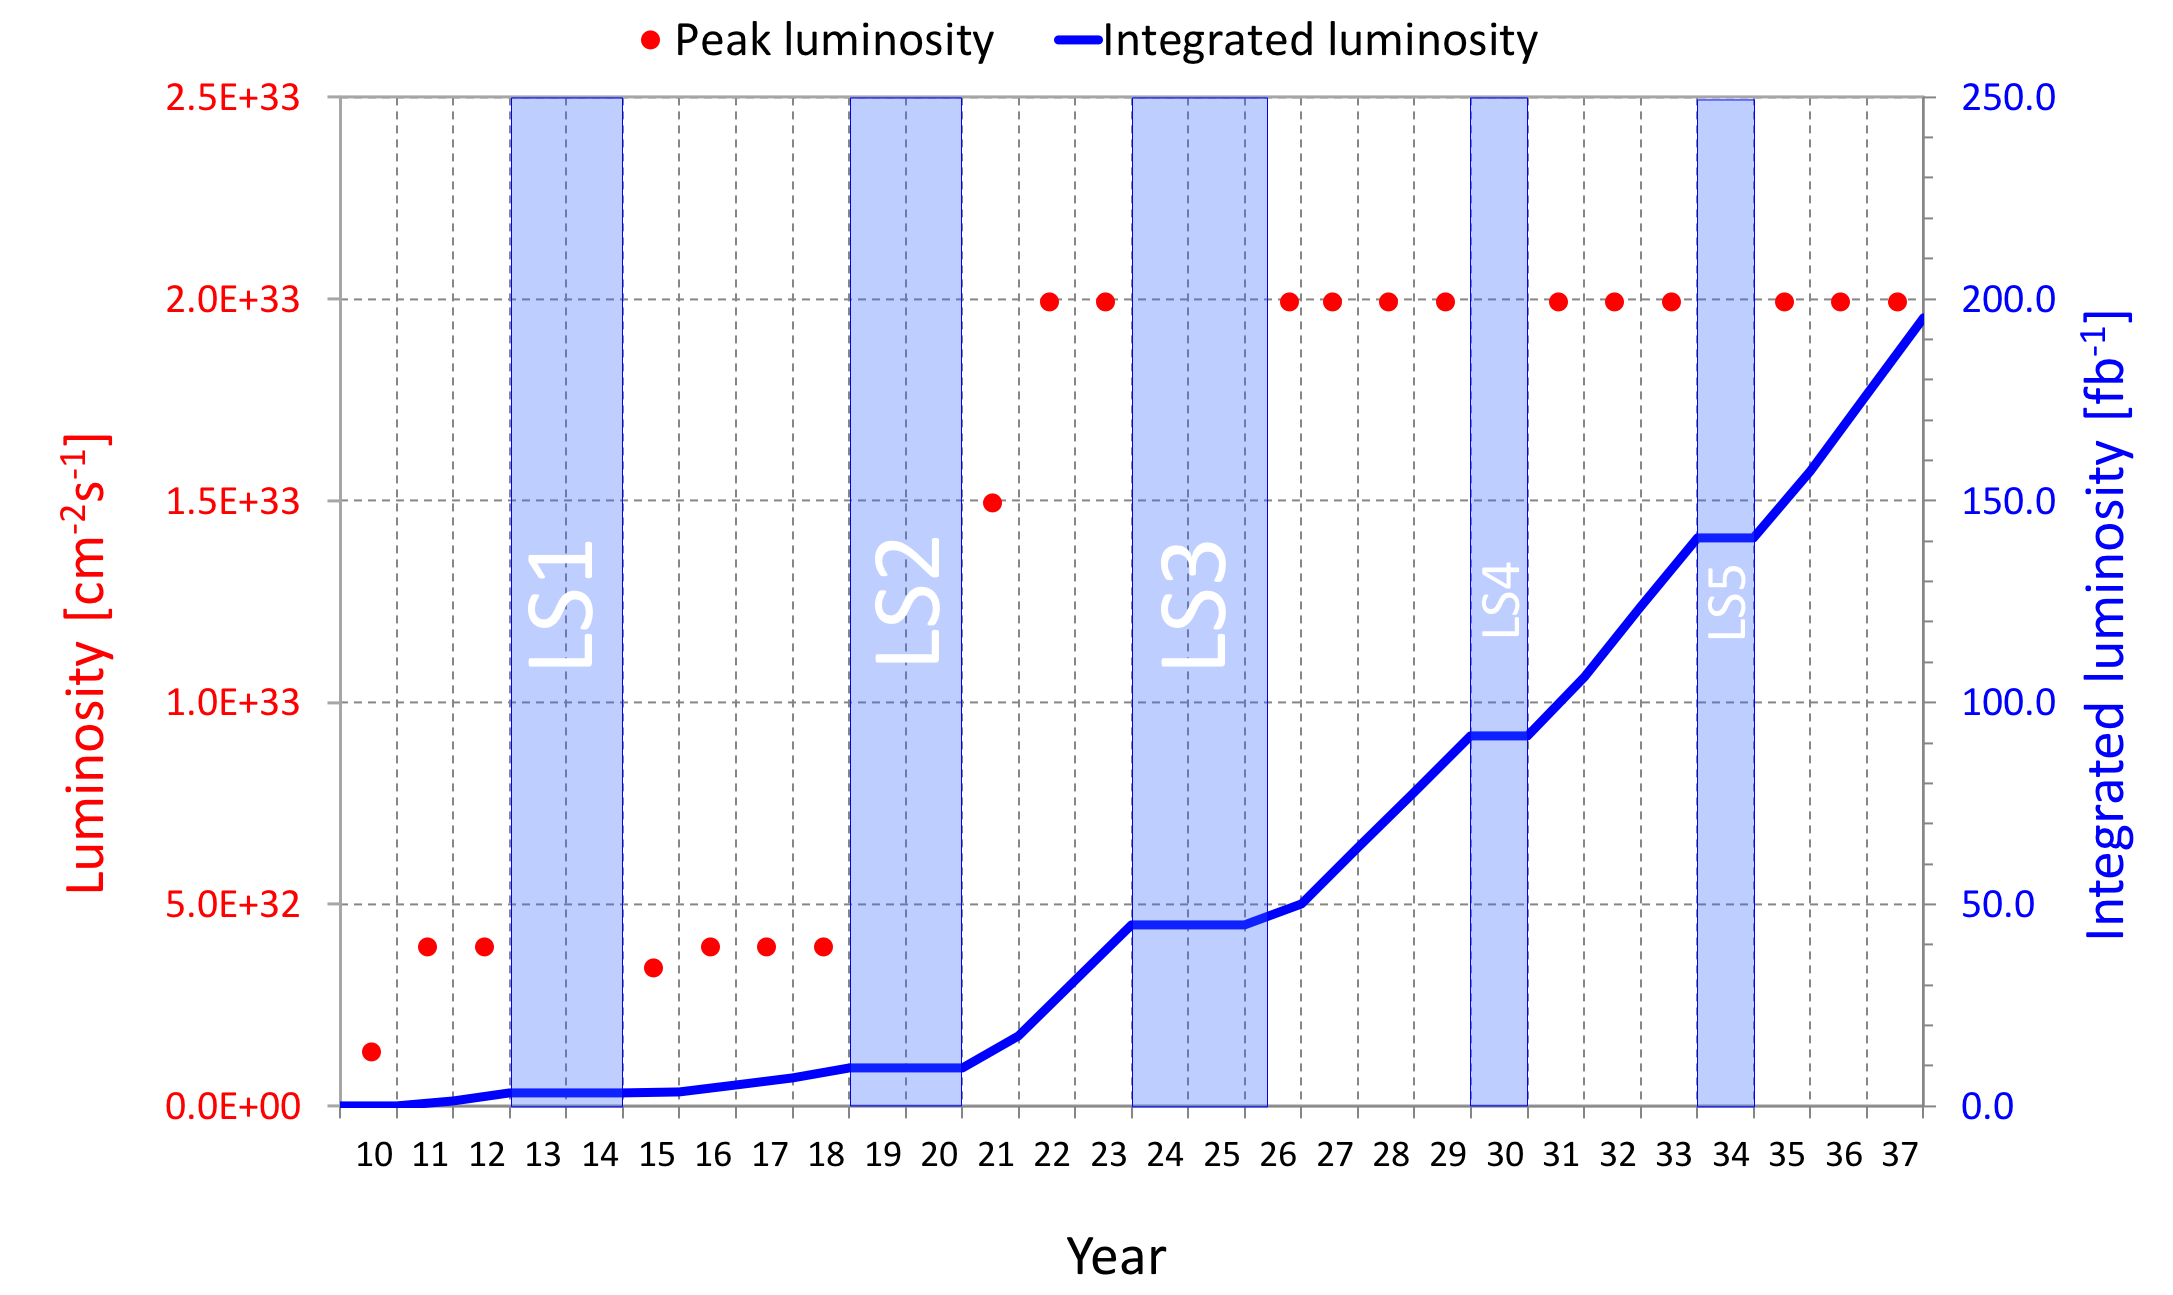
\includegraphics[width=0.9\textwidth]{Fig/fig_HGCAL/LHCb-to-2037}\\
    \caption{Projected LHC performance through 2035, with dates of long shutdowns of LHC, periods of data-taking, and projected instantaneous and integrated luminosities.}
    \label{fig:Proj}
    \end{center}
\end{figure}

\begin{figure}[!ht]
    \begin{center}  
    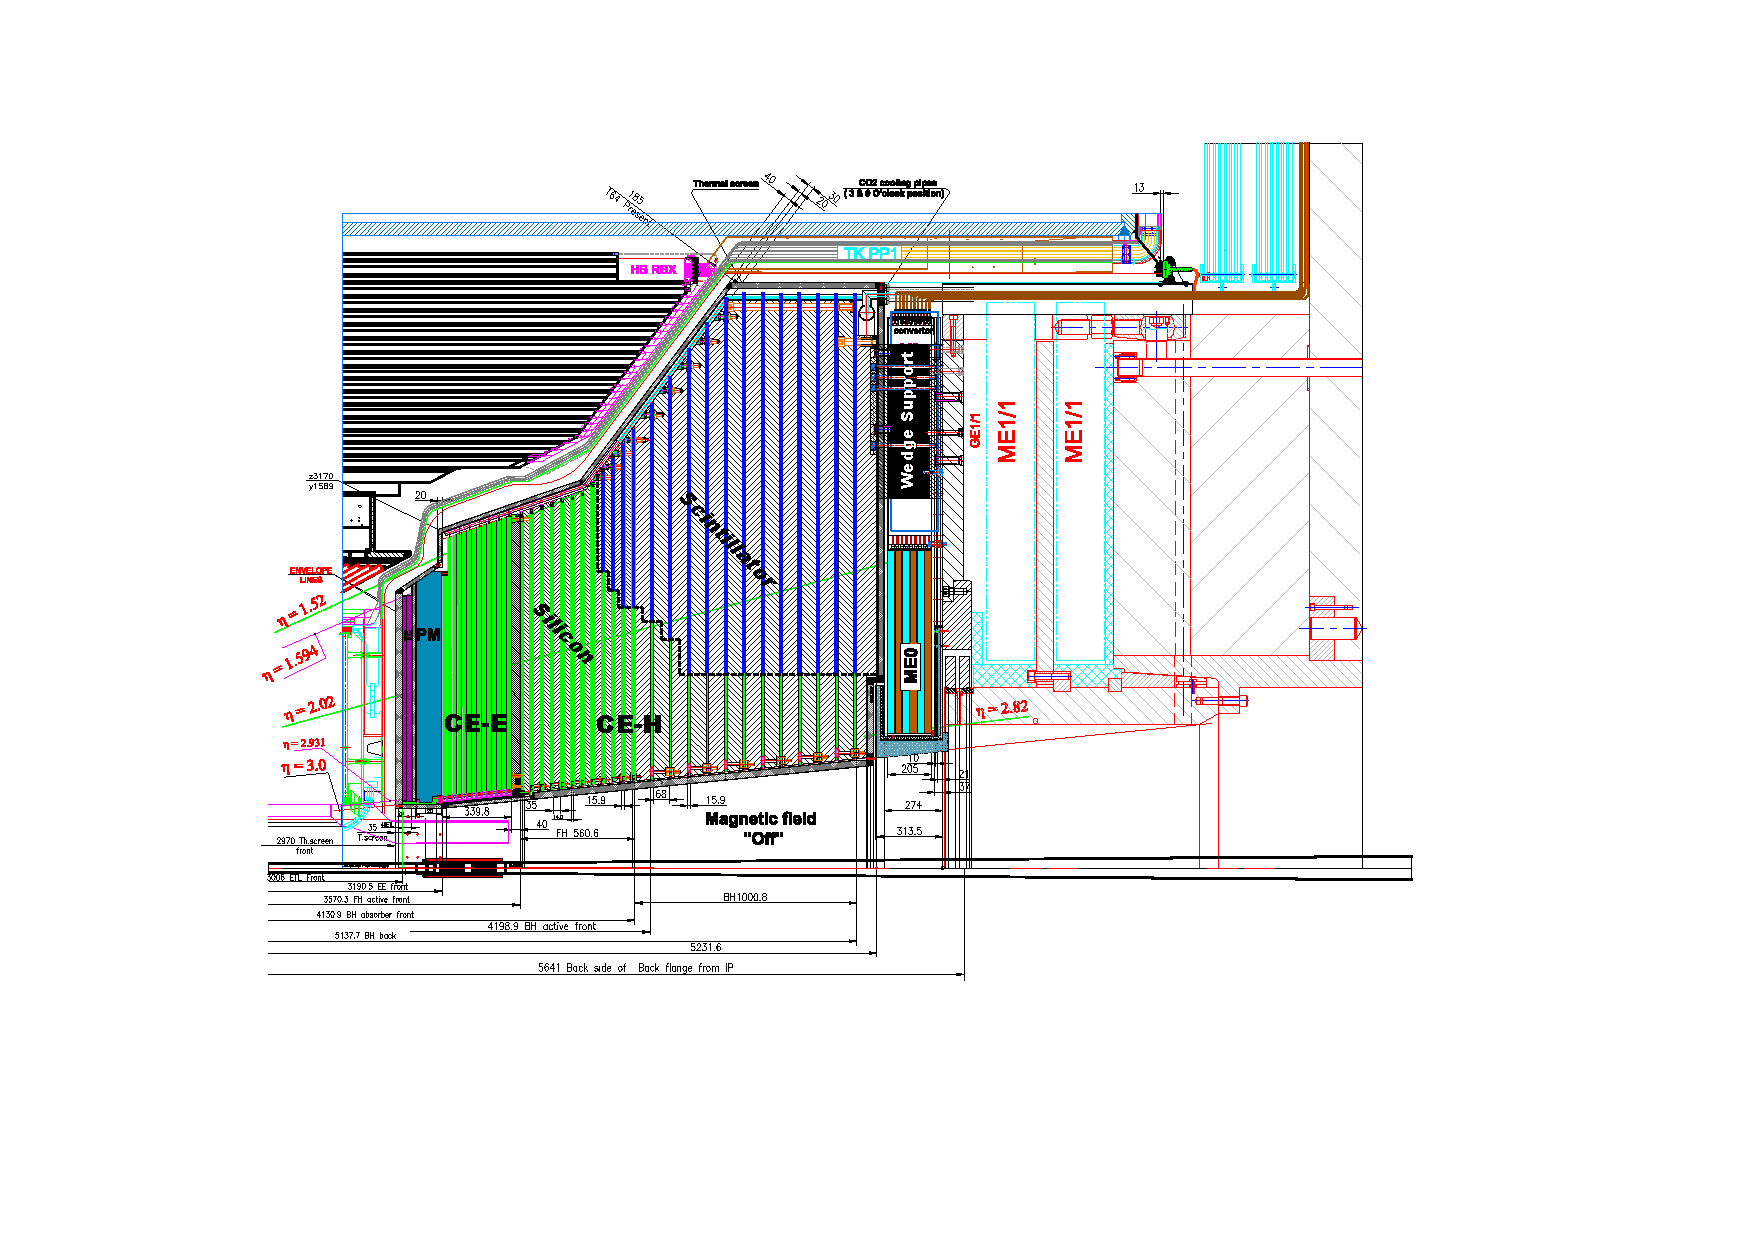
\includegraphics[width=0.9\textwidth]{Fig/fig_HGCAL/HGCAL-Longitudinal-section}\\
    \caption{Longitudinal cross section of the upper half of one endcap calorimeter~\cite{Collaboration:2293646}.}
    \label{fig:HGCAL-longitudinal}
    \end{center}
\end{figure}

In this beamtest, the HGCAL, including electromagnetic and hadronic compartments, and the analogue hadronic calorimeter (AHCAL)~\cite{collaboration:2010hb} were tested jointly. The actual setup for the beamtest is shown in Fig.~\ref{fig:Beamtest-setup}.

\begin{figure}[!ht]
    \begin{center}  
    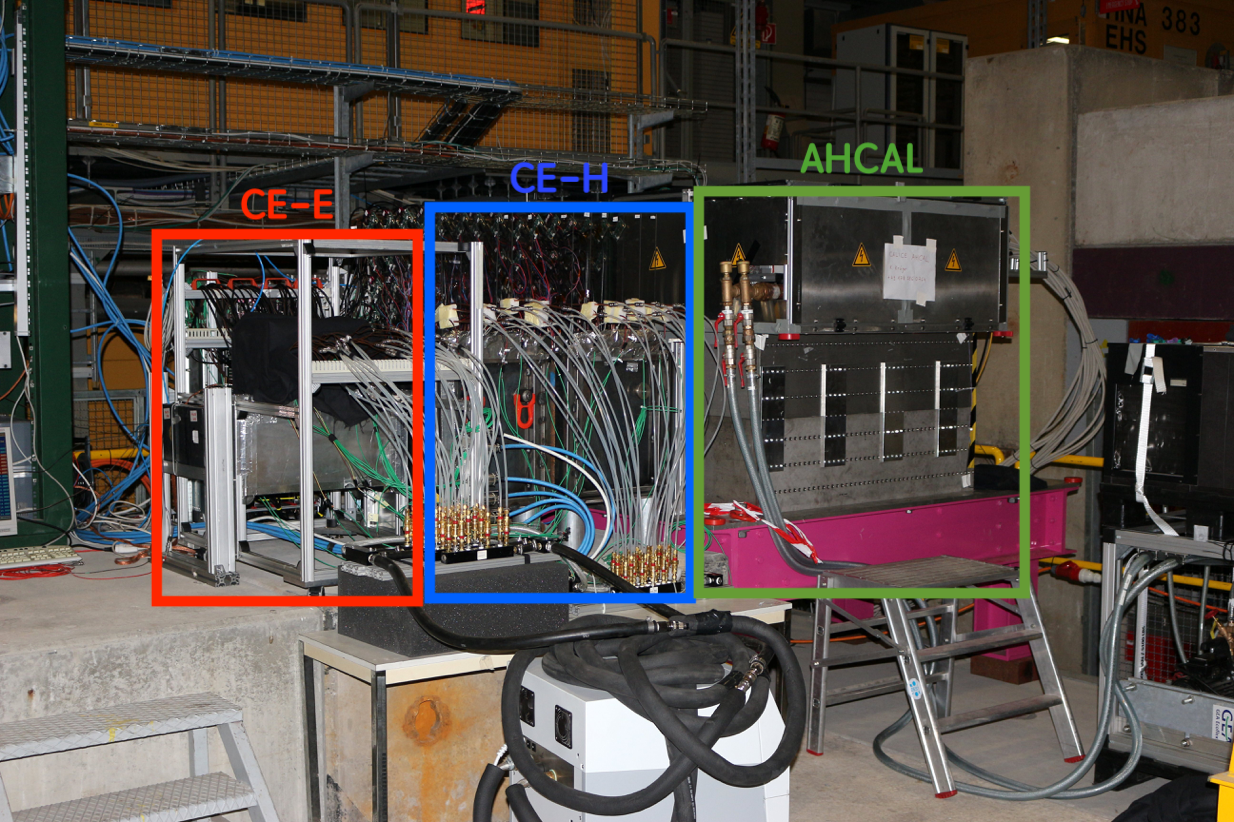
\includegraphics[width=0.9\textwidth]{Fig/fig_HGCAL/Beamtest-Oct-setup}\\
    \caption{Beamtest setup.}
    \label{fig:Beamtest-setup}
    \end{center}
\end{figure}

The simplified analysis flow is shown in Fig.~\ref{fig:data-workflow}. My analysis focuses on the energy reconstruction using boosted decision tree (BDT) method and electron identification, and mainly uses the reconstructed-level (RECO) objects. The basic element of the RECO object is the reconstructed hit (RecHit), which is energy deposit in the sensor with pedestal and common-mode (CM) noises subtracted. The definitions of the pedestal and CM noises can be found in Ref.~\cite{1748-0221-13-10-P10023} and will not be described in detail in this report. Although I participated in the October beamtest, the used datasets for the studies were taken (or simulated) from beamtest in June, where 28 layers of modules were tested.

\begin{figure}[p]
    \begin{center}  
    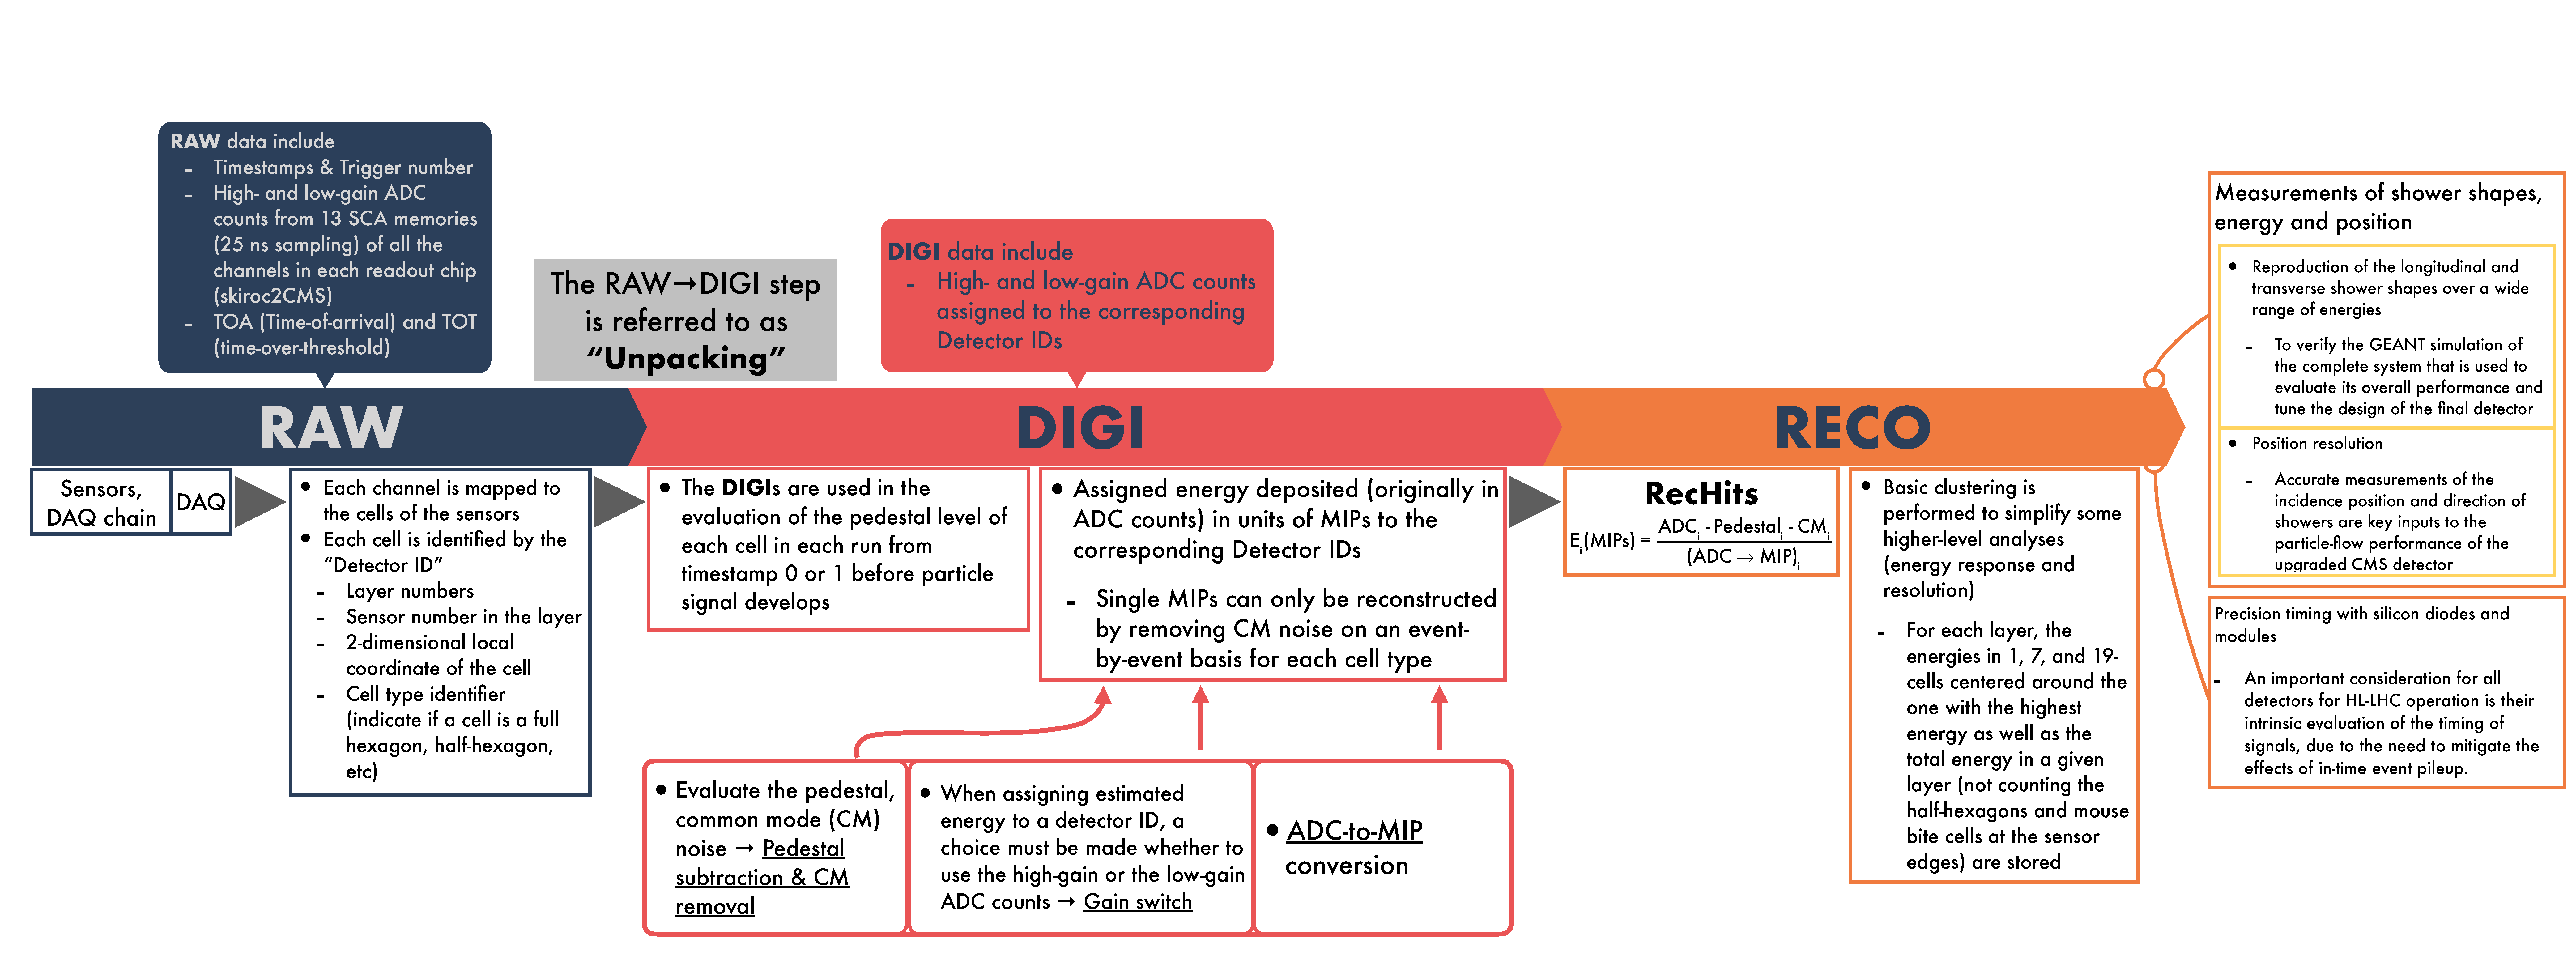
\includegraphics[angle=90,width=0.5\textwidth]{Fig/fig_HGCAL/Data-analysis-framework}\\
    \caption{The workflow of the data analysis framework, data preparation and reconstruction.}
    \label{fig:data-workflow}
    \end{center}
\end{figure}

\section{BDT method for energy reconstruction}
\label{sec:energyreconstruction}
The study aims at comparing various methods for energy reconstruction. My study focuses on the electron. The strategy is to use the simulation samples for regression, and the final goal is to apply the training result on beamtest data.
In previous beamtests, the energy of the shower was calculated as the sum of the energy deposits in the active silicon sensors and in the passive absorbers over all tested layers, where the energy deposits in the absorbers were estimated using the stopping power\footnotemark of the absorber materials which can be obtained from PDG~\cite{PhysRevD.98.030001} and simulation. \footnotetext{The energy losses per unit length (dE/dx) of certain particle in the given material.}
In the following text, I will refer to this method as dEdx method. The full description of this method can be found in Ref.~\cite{1748-0221-13-10-P10023}. 


This study uses the XGBRegressor in XGBoost library~\cite{XGBoost-Documentation}, where the Gradient Boosting algorithm is implemented. The hyper-parameters adopted are listed in Table.~\ref{tab:hyperparam}

\begin{table}[!ht]
  \begin{center}
    {
    \begin{tabular}{lc}
    	hyperparameter & Parameters value\\
    	\hline
    	n\_estimators & 500 \\
    	learning\_rate & 0.08 \\
    	gamma & 0 \\
    	subsample & 0.75 \\
    	colsample\_bytree & 1 \\
    	max\_depth & 7 \\
    \end{tabular}
    }
  \end{center}
  \caption{The hyper-parameters adopted in the XGBRegressor for the regression.  \label{tab:hyperparam}}
\end{table}

The definitions of variables used to construct training features are listed in Table.~\ref{tab:regression_feature}.

\begin{table}[!ht]
  \begin{center}
    {\small
    \begin{tabular}{lc}
    	Variable &  Definition \\
    	\hline
    	EAll & Energy deposits in each layer \\
    	Etot & Energy deposits in all layers \\
    	sum1 & Energy deposit of the most energetic cell in each layer\\
    	sum7 & Energy deposits in 7 cells centered at the most energetic cell in each layer\\
    	sum19 & Energy deposits in 19 cells centered at the most energetic cell in each layer\\
    \end{tabular}
    }
  \end{center}
  \caption{The variables used to construct training features for the regression.  \label{tab:regression_feature}}
\end{table}

Each layer has individual value for EAll, sum1, sum7, and sum19. From these basic variables, one can further construct simple lateral shower shape variables, such as sum1/sum7 (referred to as E1/E7), sum7/sum19 (E7/E19), and sum1/sum19 (E1/E19). 

In the very first test~\cite{Ryan-ERecoBDT}, only the variables EAll and EAll/Etot were used as training features (for total of 56 variables) with the beam energy as target. Two sets of training were studied, one with the trained dataset having a uniform energy profile, and the other one with certain energy range ($\pm 10\GeV$) for each energy point. Fig.~\ref{fig:energyreco-bdt-Ryan} shows the results of the relative resolution as a function of predicted beam energy from regression (left) and the energy response as a function of predicted beam energy (right). 
The relative resolution is defined as the width of the reconstructed energy distribution divided by the predicted beam energy, while the energy response is defined as the ratio between the mean value of the reconstructed energy distribution and the true beam energy. Examples of the reconstructed energy distributions are shown in Fig.~\ref{fig:energyreco-distributions}. 
The observations from Fig.~\ref{fig:energyreco-bdt-Ryan} and ~\ref{fig:energyreco-distributions} are
\begin{itemize}  
\item On the left plot, one clearly sees that results of relative resolution obtained from both sets of training are poorer than that from dEdx method, and the differences are larger at low energy points than at high energy points.
\item The differences can be reduced with the training with energy range, indicating that at low energy points the predictions from regression are less precise, and the precision can be improved with the training with energy window.  
\item Although BDT regression gives worse resolutions than dEdx method, the scale of the reconstructed energy is more precise and gives more linear response, as can be seen on right plot.  
\item From the reconstructed energy distributions, one can see that the distributions are non-Gaussian and there are low energy outliers. By looking at the event displays, as shown in Fig.~\ref{fig:EvDisplay1}, the showers from events with low predicted energy (bottom plot, where the prediced energy is 15.8\GeV) do not develop as deep as those from normal predicted energy events (top plot, where the prediced energy is 20.1\GeV). Apart from this observation, there are few events where the electron hits the edge of the hexagon. However, rejecting events where the hit with the maximum energy deposit in the first layer is outside the $2\unit{cm}\times 2\unit{cm}$ area around the hexagon center has marginal impact on the reconstructed energy distribution.
\end{itemize}

\begin{figure}[!ht]
    \begin{center}  
    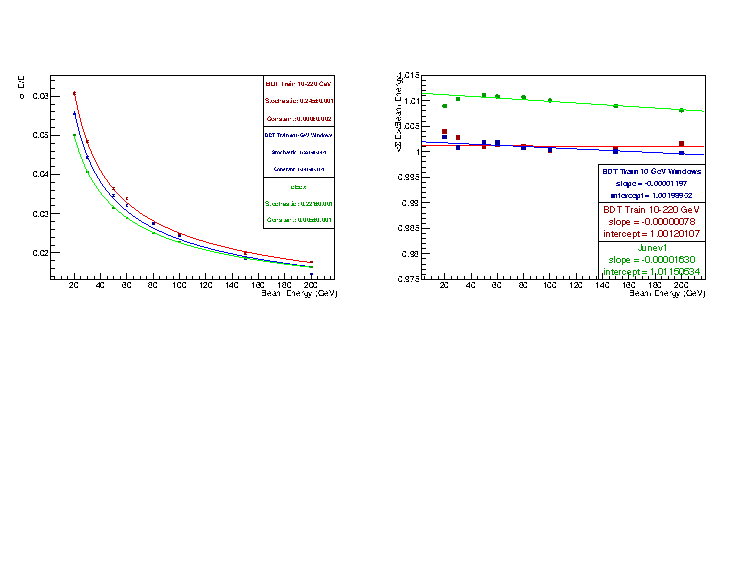
\includegraphics[width=1.0\textwidth]{Fig/fig_HGCAL/energyreco-bdt-Ryan} \\
    \caption{Results of the relative resolution as a function of predicted beam energy from regression (left) and the energy response as a function of predicted beam energy (right).}
    \label{fig:energyreco-bdt-Ryan}
    \end{center}
\end{figure}

\begin{figure}[!ht]
    \begin{center}  
    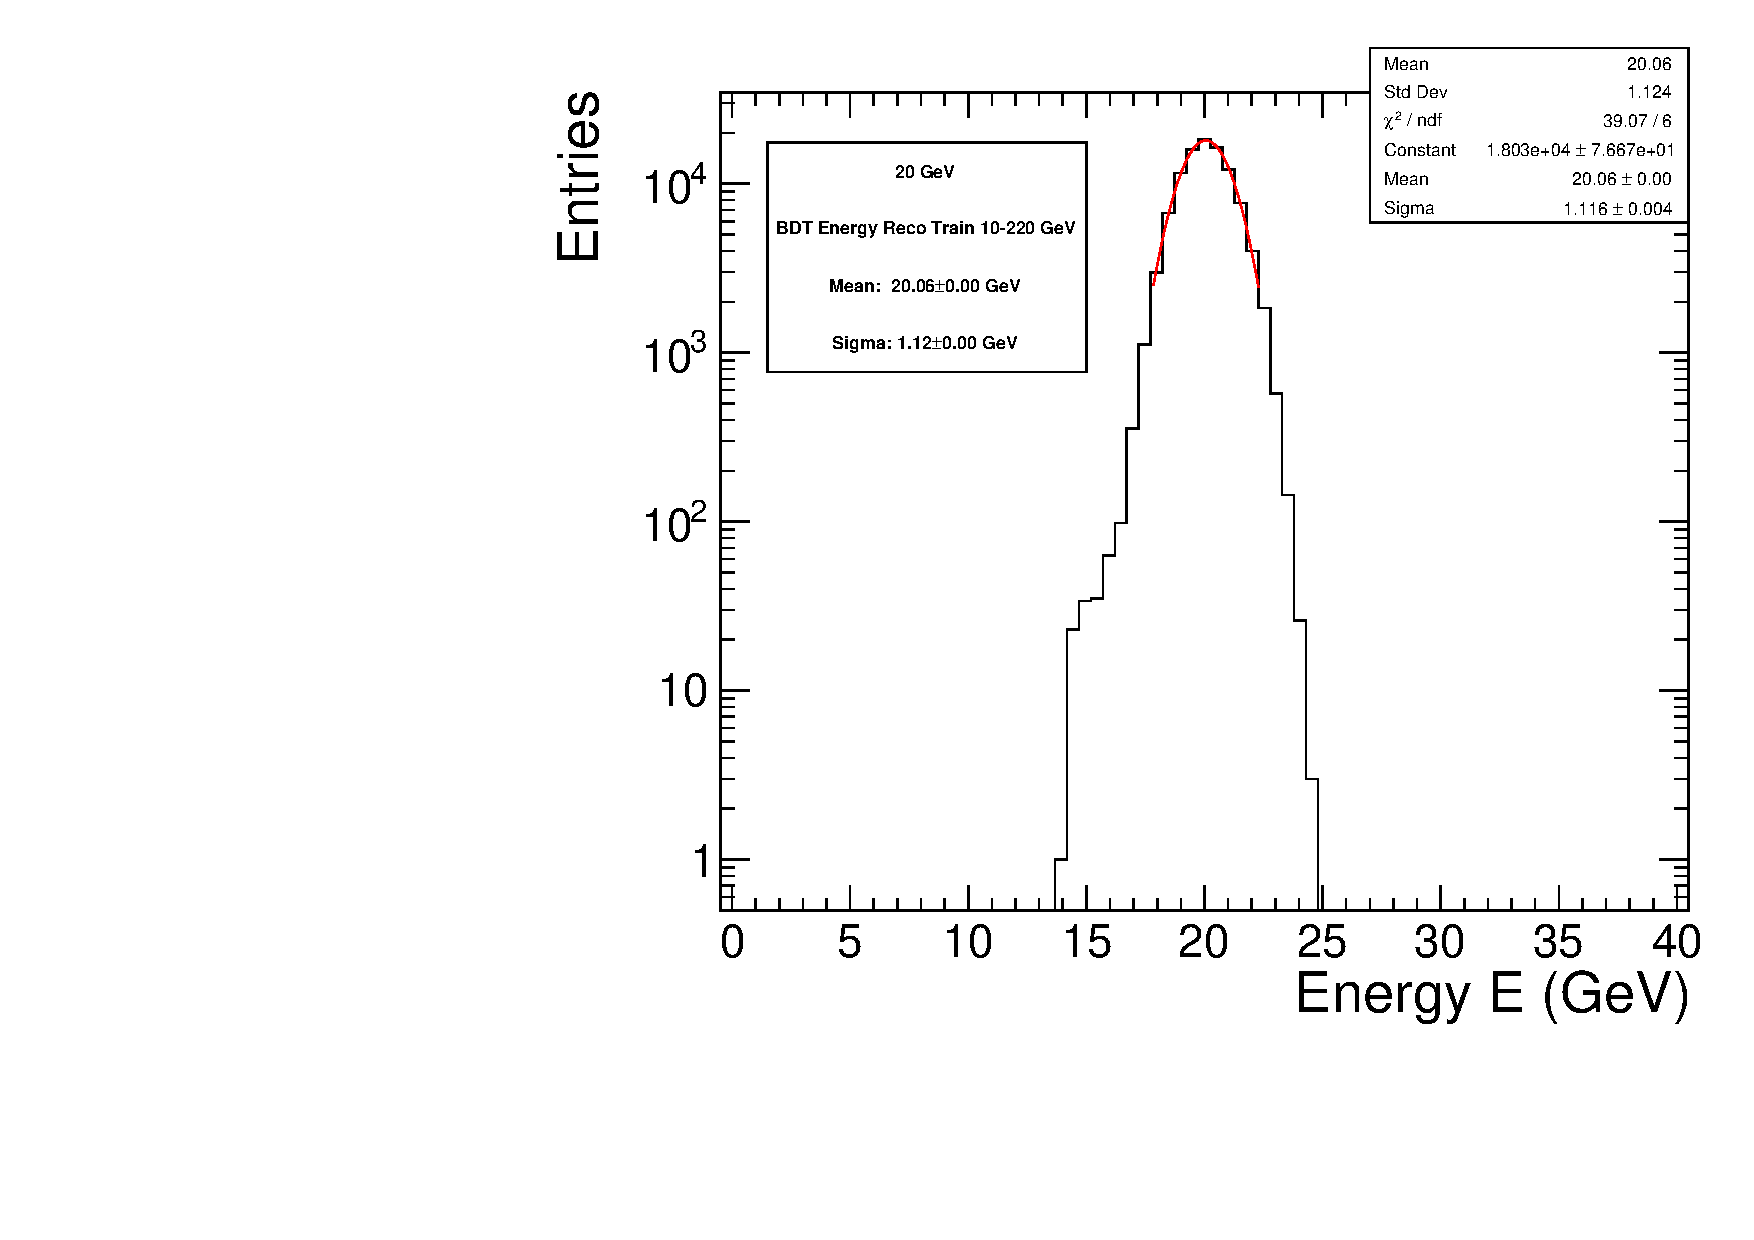
\includegraphics[width=0.49\textwidth]{Fig/fig_HGCAL/Energy_pred_dynamic_windowed_showershape_v2_20GeV}~
    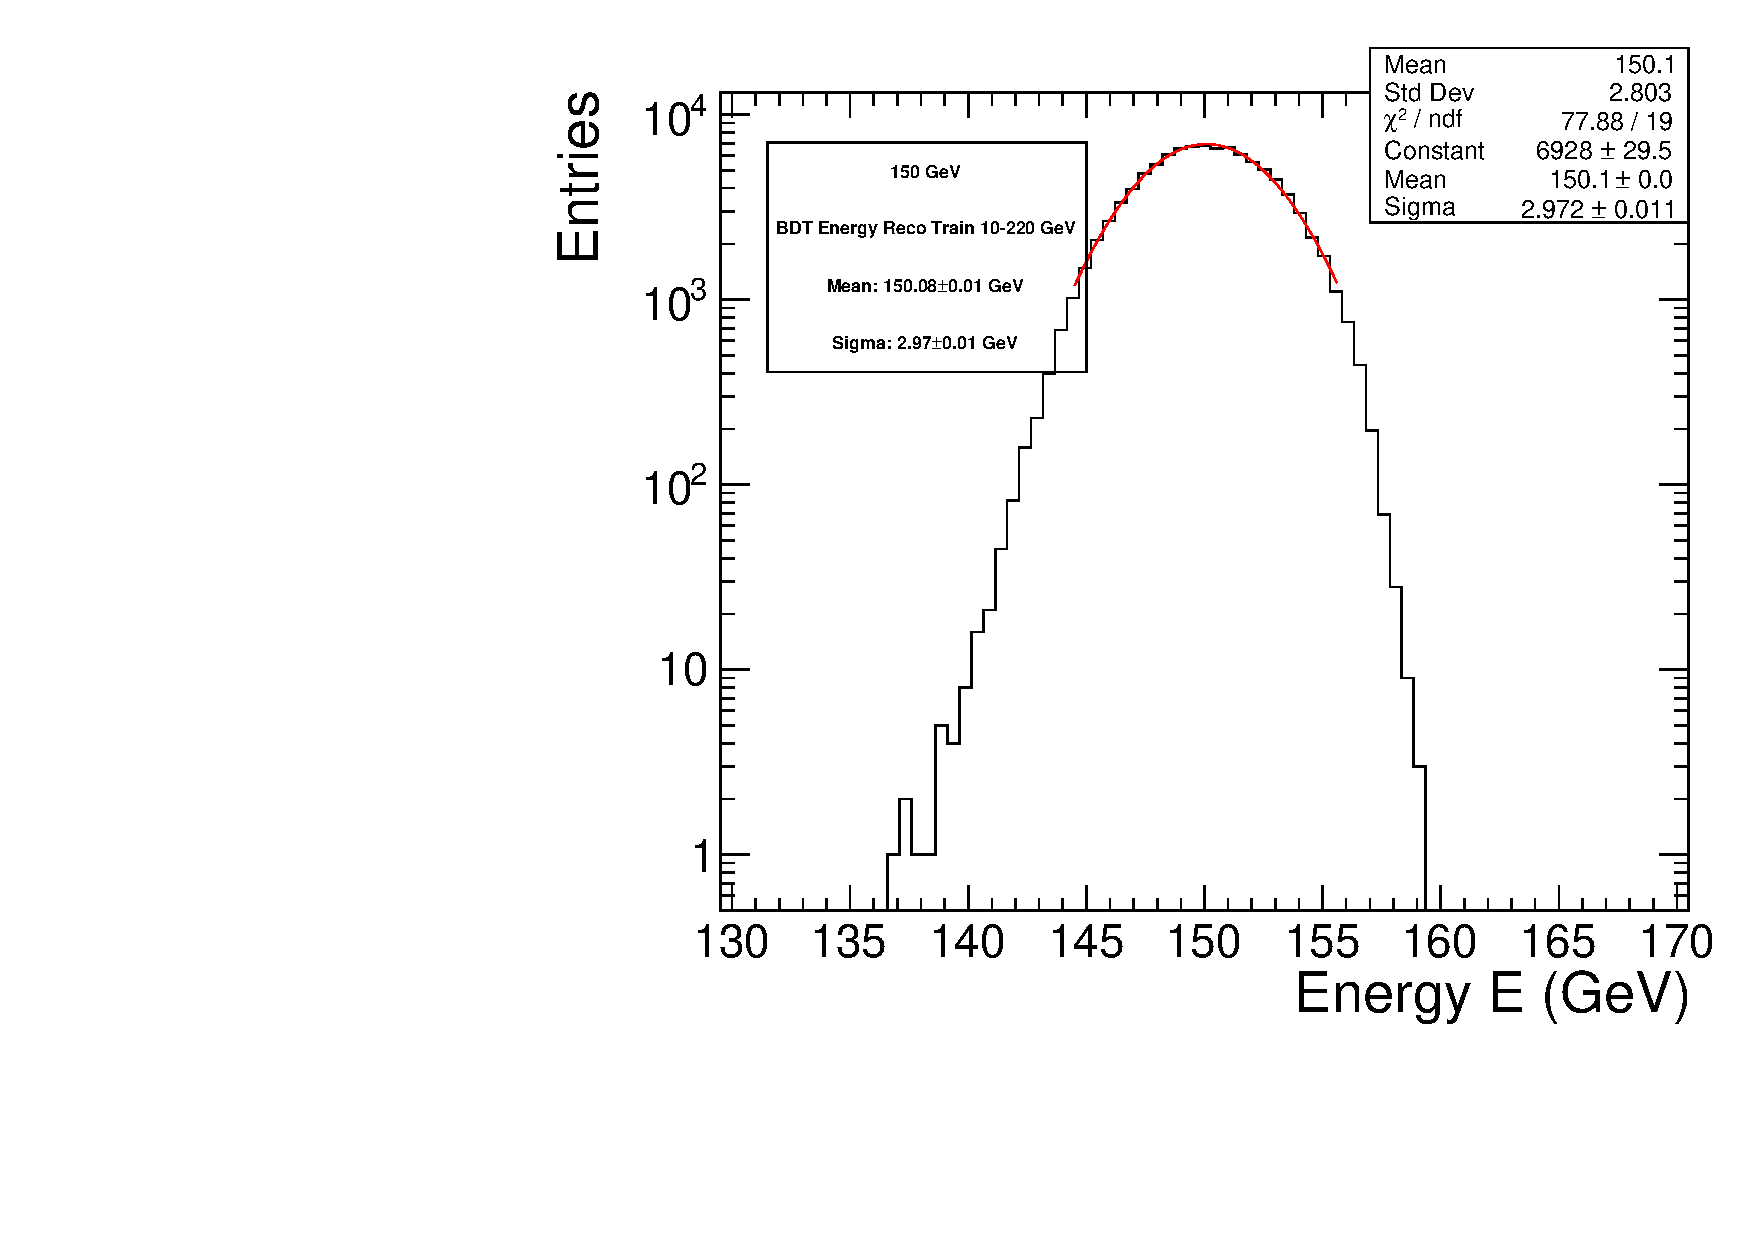
\includegraphics[width=0.49\textwidth]{Fig/fig_HGCAL/Energy_pred_dynamic_windowed_showershape_v2_150GeV}\\
    \caption{Reconstructed energy distributions for 20\GeV electrons (left) and 150\GeV electrons (right) predicted from regression.}
    \label{fig:energyreco-distributions}
    \end{center}
\end{figure}

\begin{figure}[p]
    \begin{center}  
    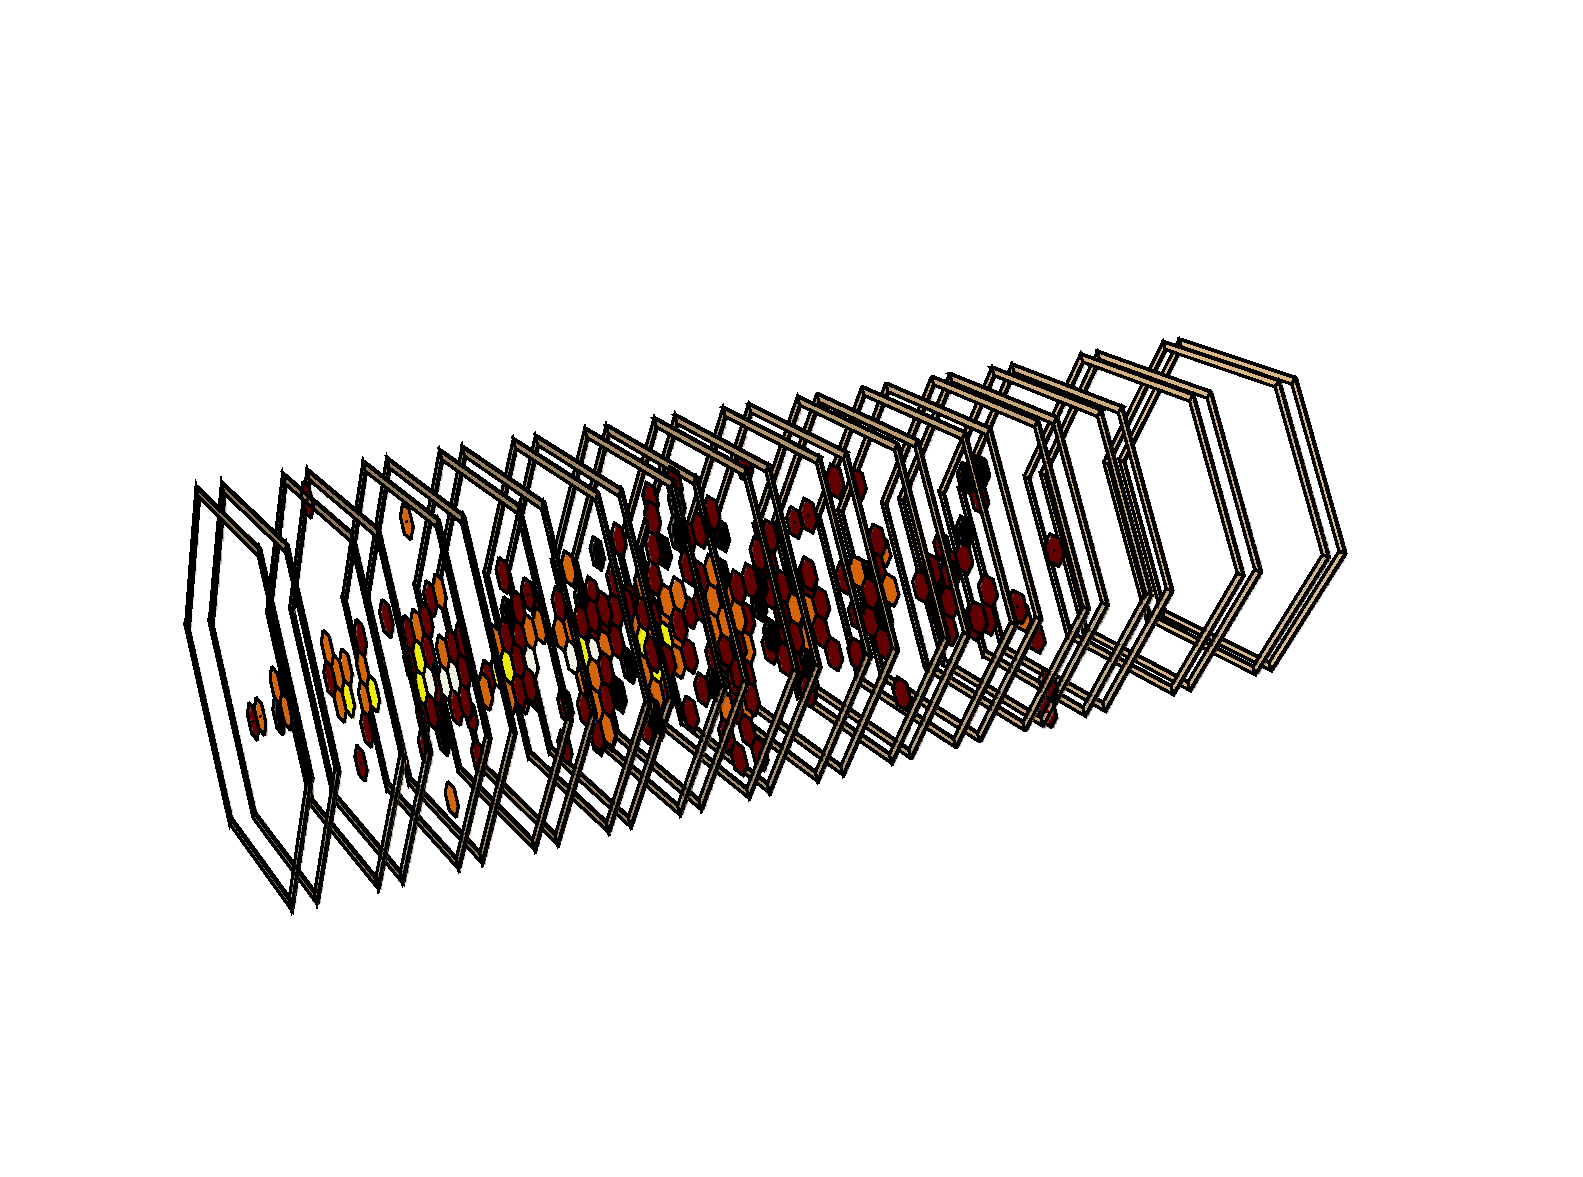
\includegraphics[width=1.0\textwidth]{Fig/fig_HGCAL/EvDisplay3D-simulation-Junev1-Ele20GeV-TBGenSim1-event2}\\
    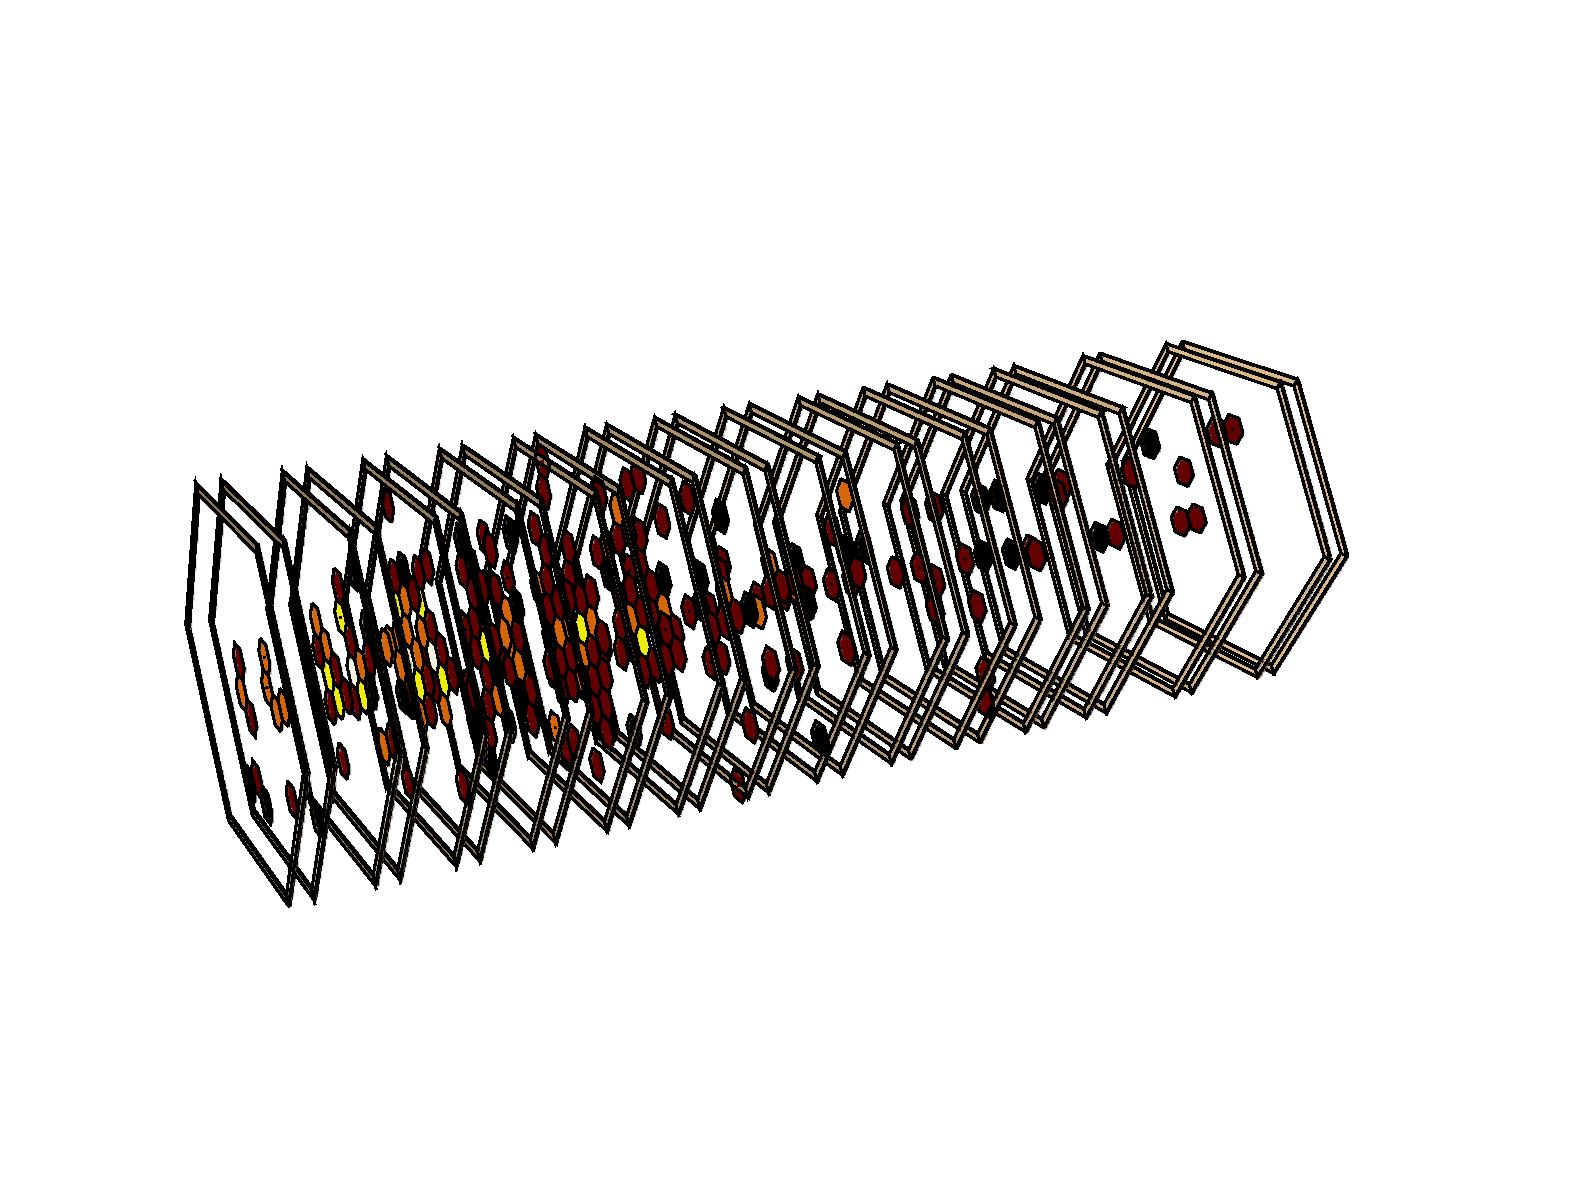
\includegraphics[width=1.0\textwidth]{Fig/fig_HGCAL/EvDisplay3D-simulation-Junev1-Ele20GeV-TBGenSim1-event1012}\\
    \caption{Examples of event display of the electron shower. The predicted energy for the shower in top plot is 20.1\GeV, while that in bottom plot is 15.8\GeV.}
    \label{fig:EvDisplay1}
    \end{center}
\end{figure}

New sets of regression are tested with (1) adding in other variables, such as lateral shower shape variables, as training features, and (2) dynamic energy window (i.e., narrower range for low energy points). Two sets of dynamic energy window are used, and are summarized in Table.~\ref{tab:EnergyWindowSize}. The feature importances of the regression for all energy points are shown in Fig.~\ref{fig:featimp_EReco}. Some interesting observations are summarized in the following list.
\begin{itemize}  
\item The pattern of the feature importance for each energy point are different from each other. 
\item EAll is the most important one among the five types of variables. 
\item E7/E19 is the most important lateral shower shape variable, compared to other two.
\item For the low energy points, the contributions of the features from variables in last few layers are marginal. 
\item For the high energy points, the importances of EAll and EAll/Etot increase between layer 7 and 12, while the importances of E1/E19 and E1/E19 decrease between layer 4 and 10 and then increase onward.
\end{itemize}

\begin{figure}[p]
    \begin{center}  
    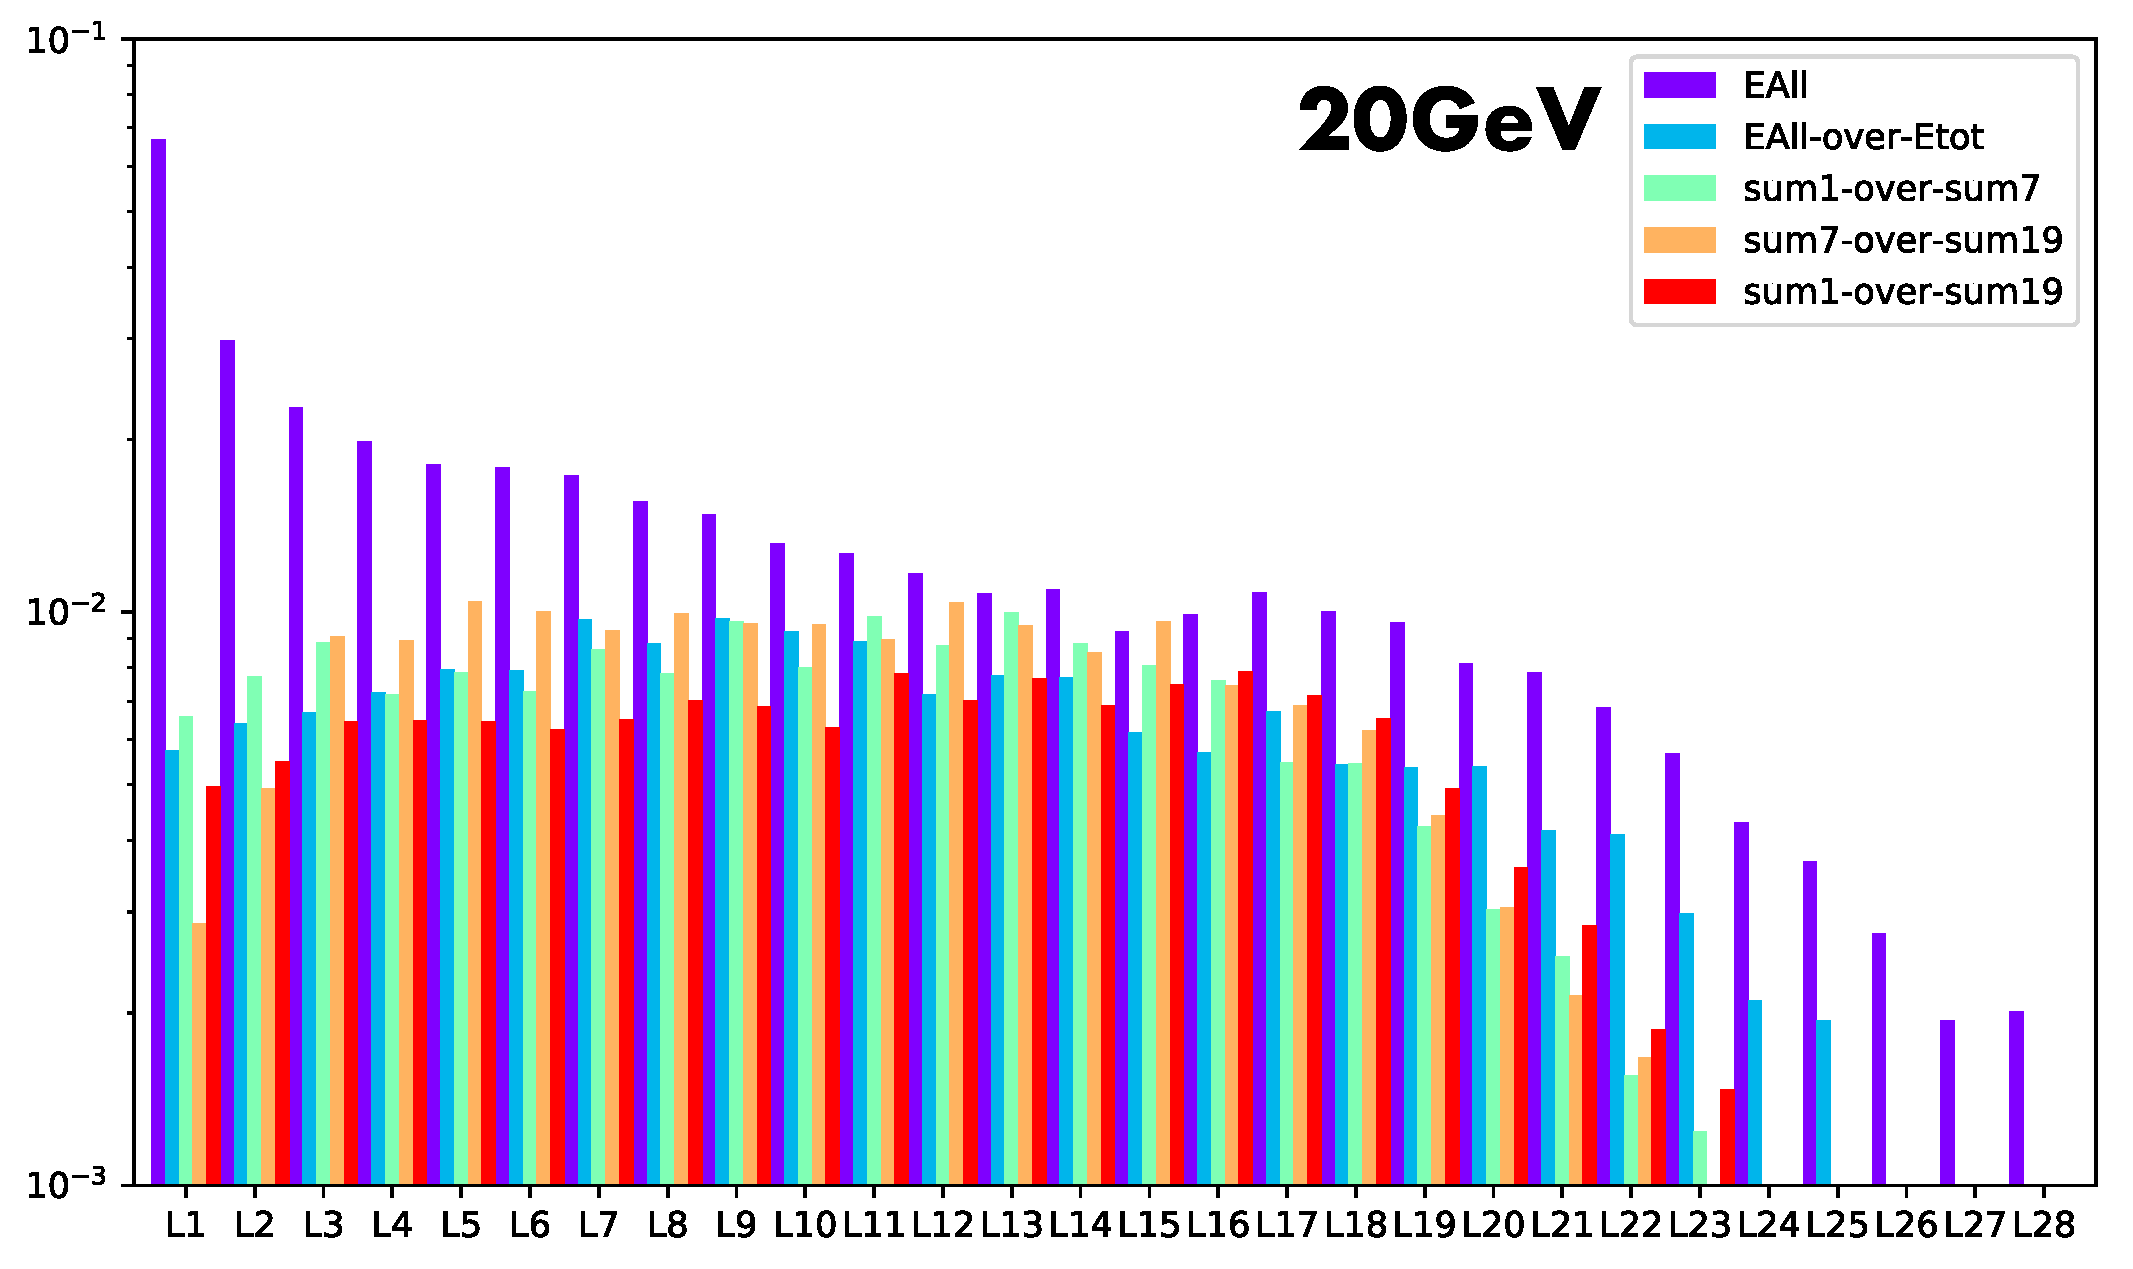
\includegraphics[width=0.5\textwidth]{Fig/fig_HGCAL/Feature_importance_showershape_dynamicwindow_v2_20GeV}~
    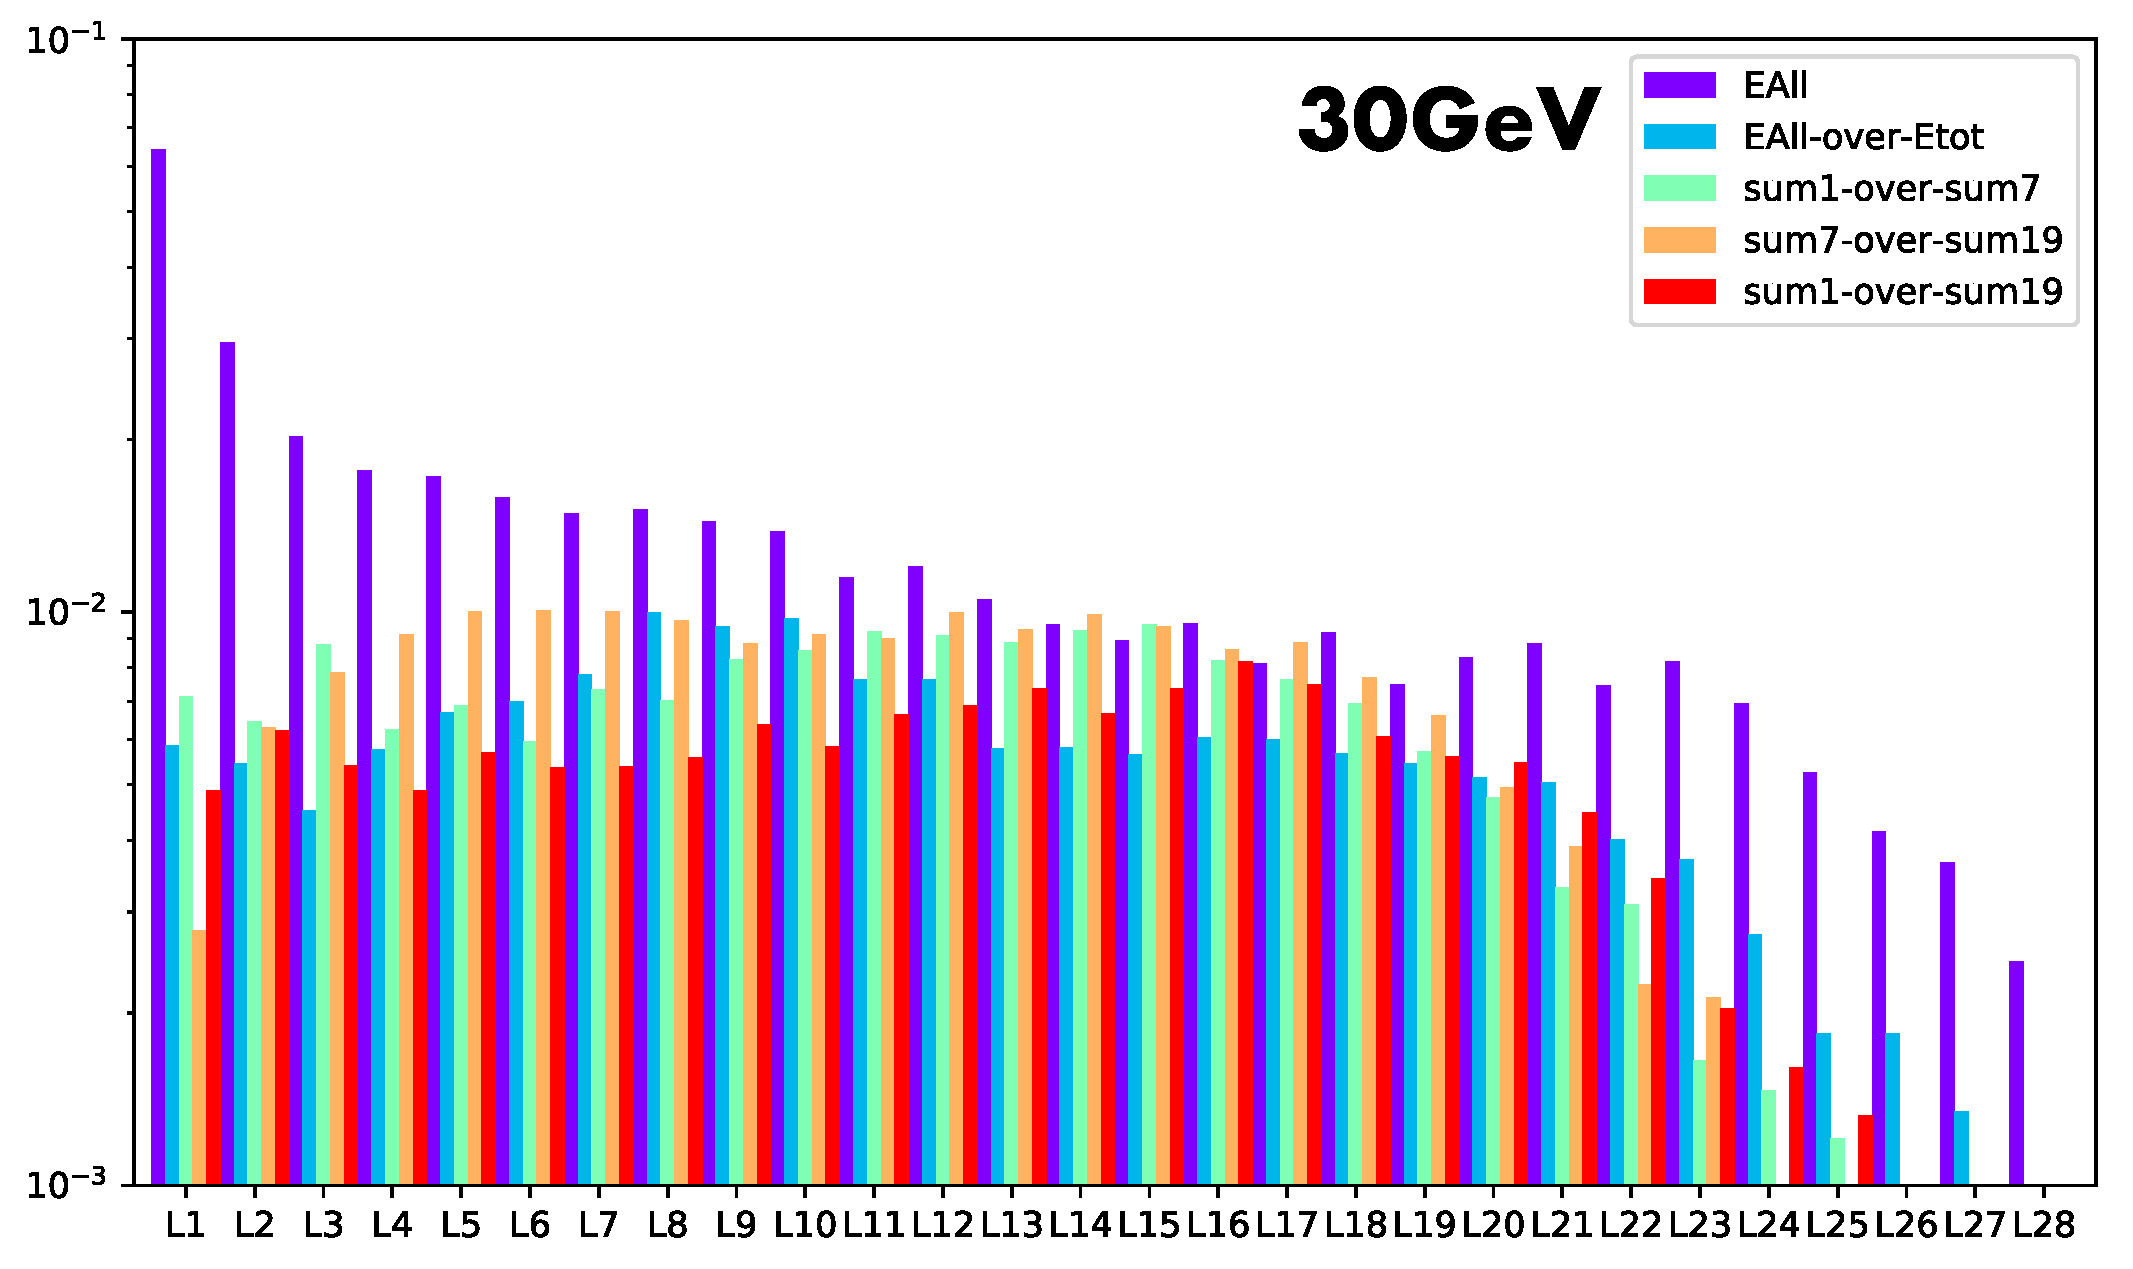
\includegraphics[width=0.5\textwidth]{Fig/fig_HGCAL/Feature_importance_showershape_dynamicwindow_v2_30GeV}\\
    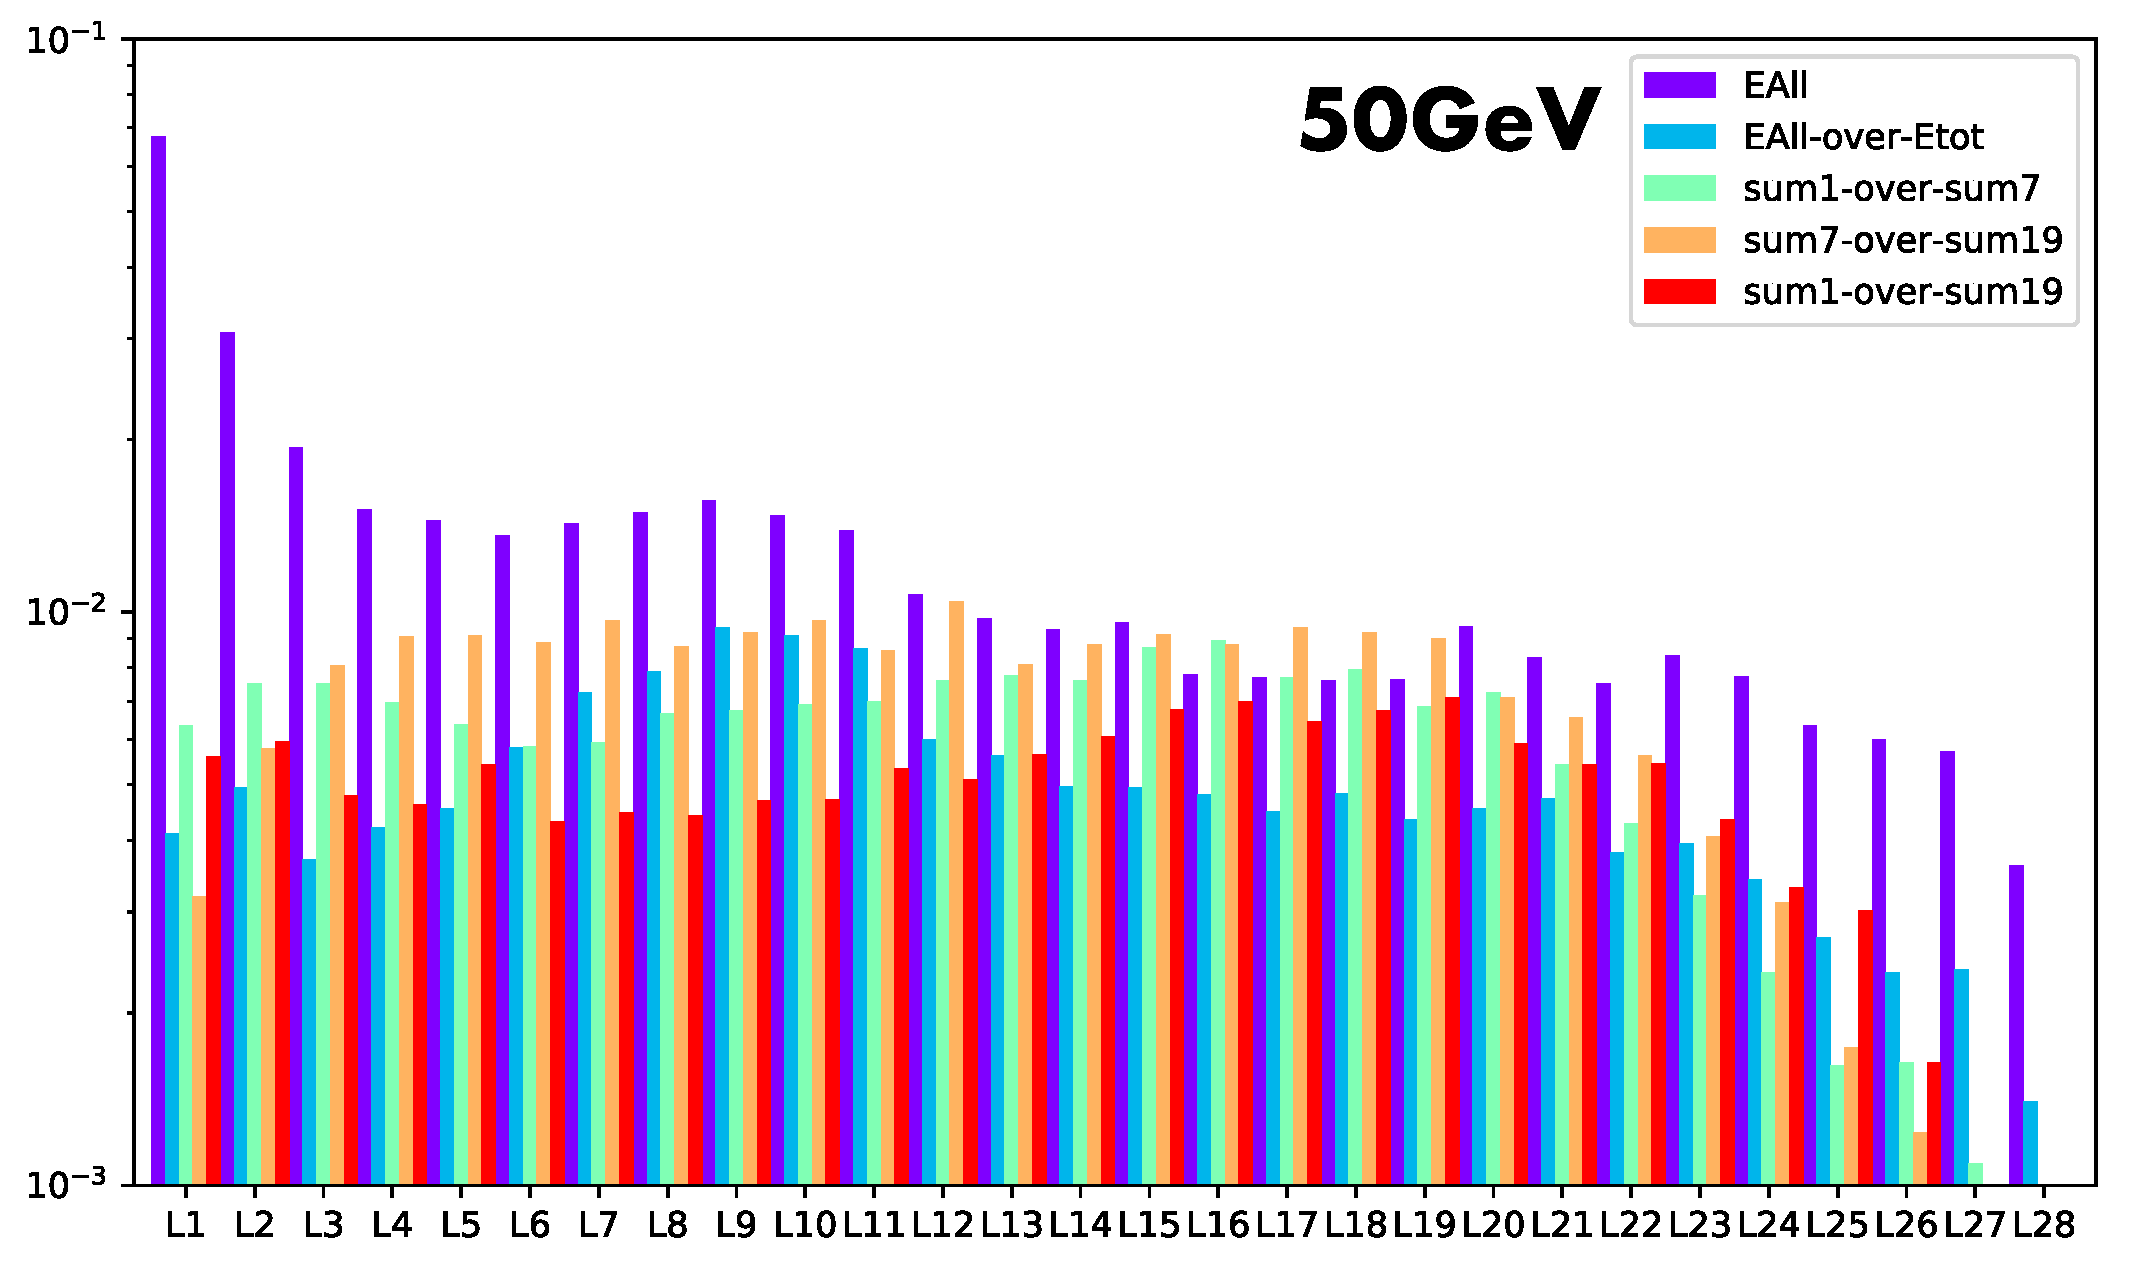
\includegraphics[width=0.5\textwidth]{Fig/fig_HGCAL/Feature_importance_showershape_dynamicwindow_v2_50GeV}~
    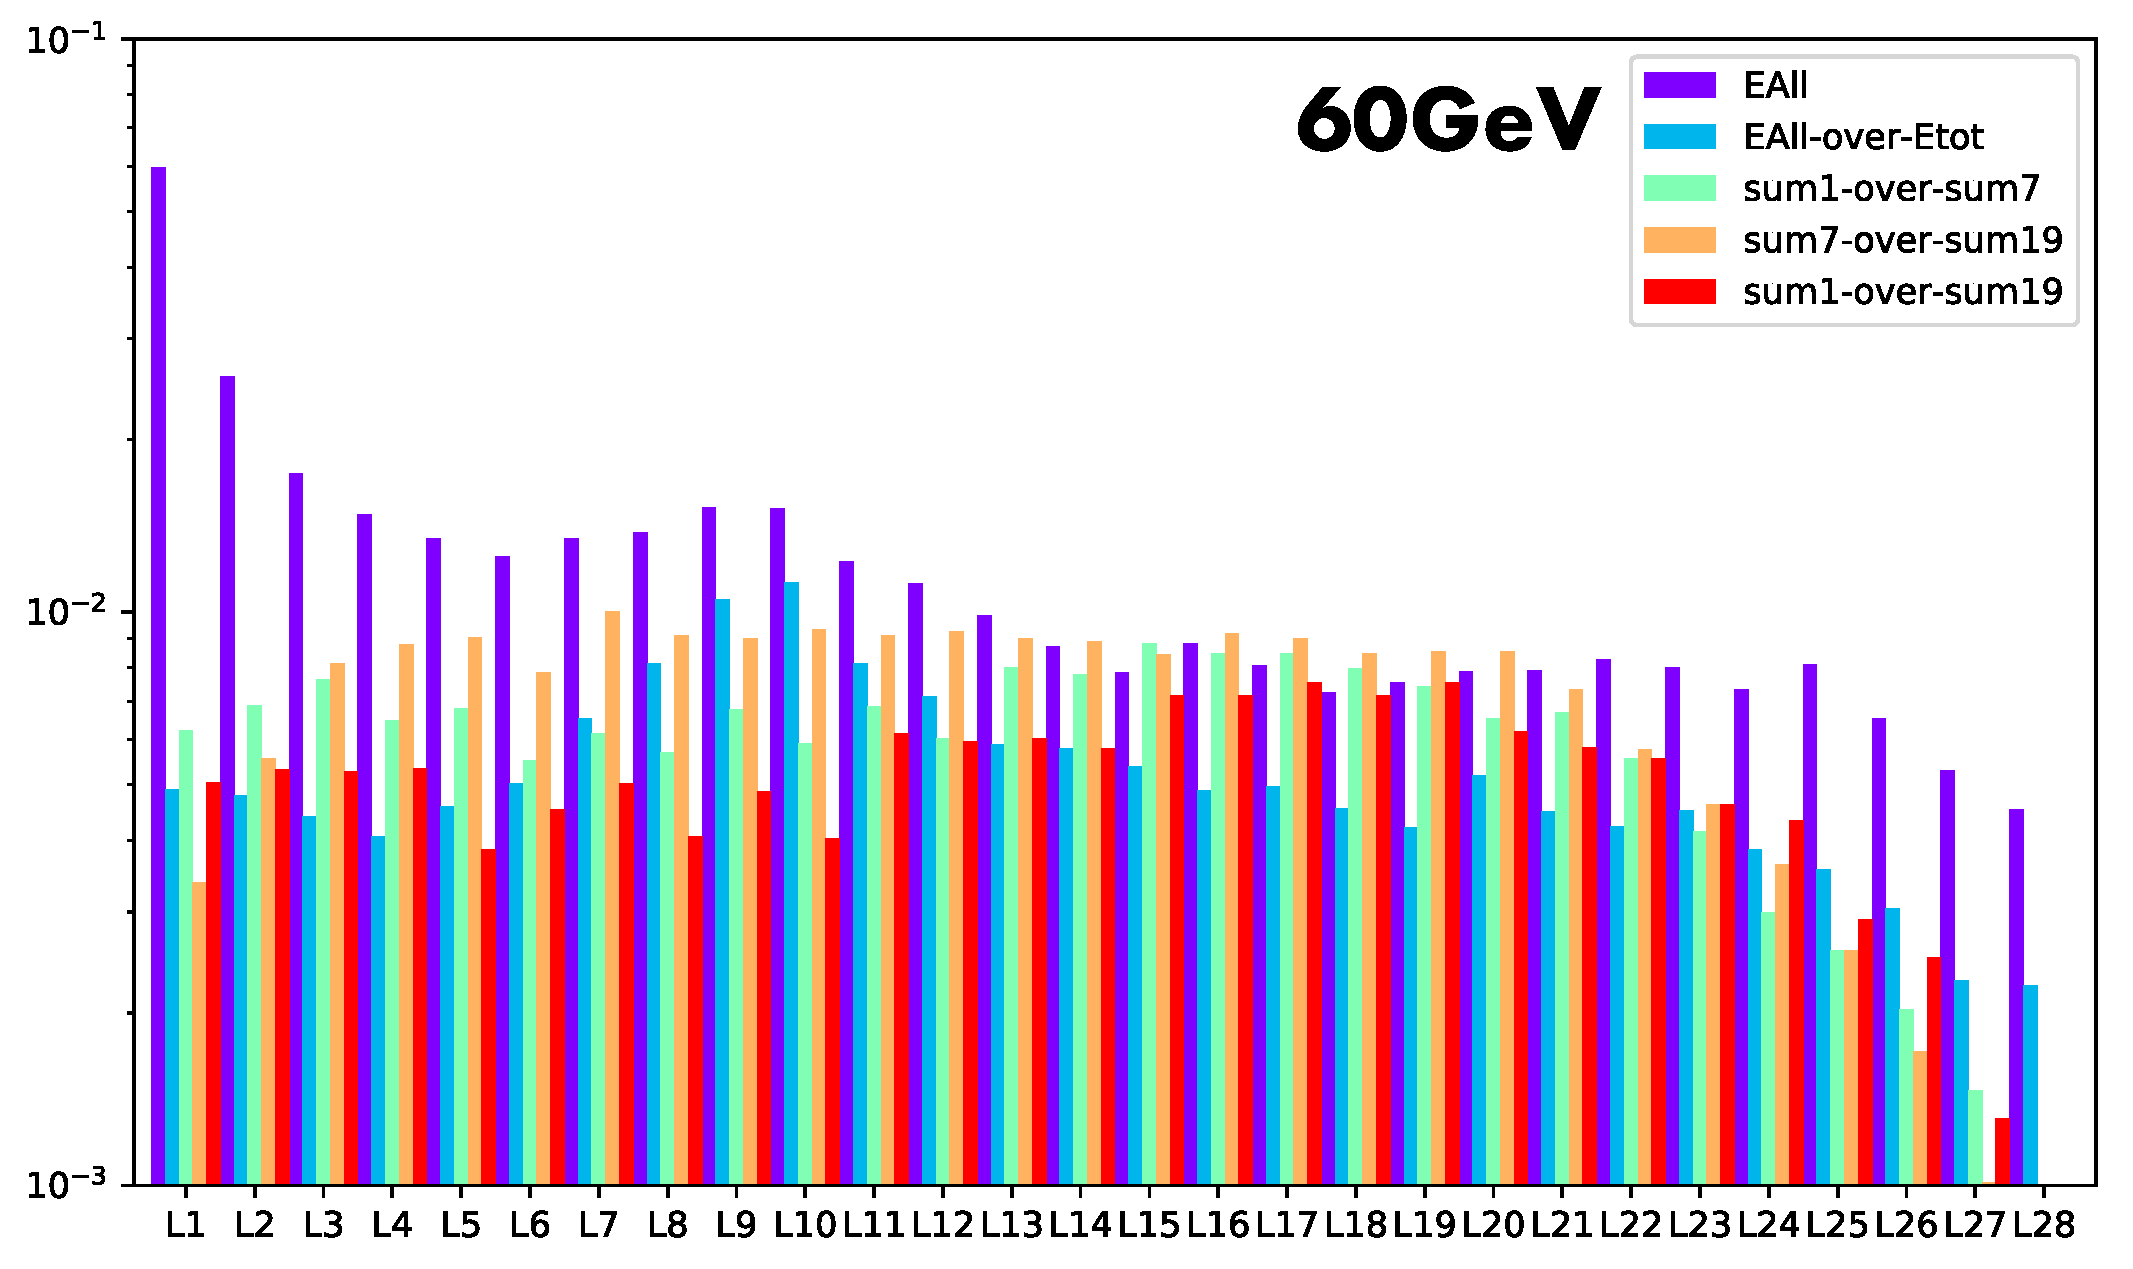
\includegraphics[width=0.5\textwidth]{Fig/fig_HGCAL/Feature_importance_showershape_dynamicwindow_v2_60GeV}\\
    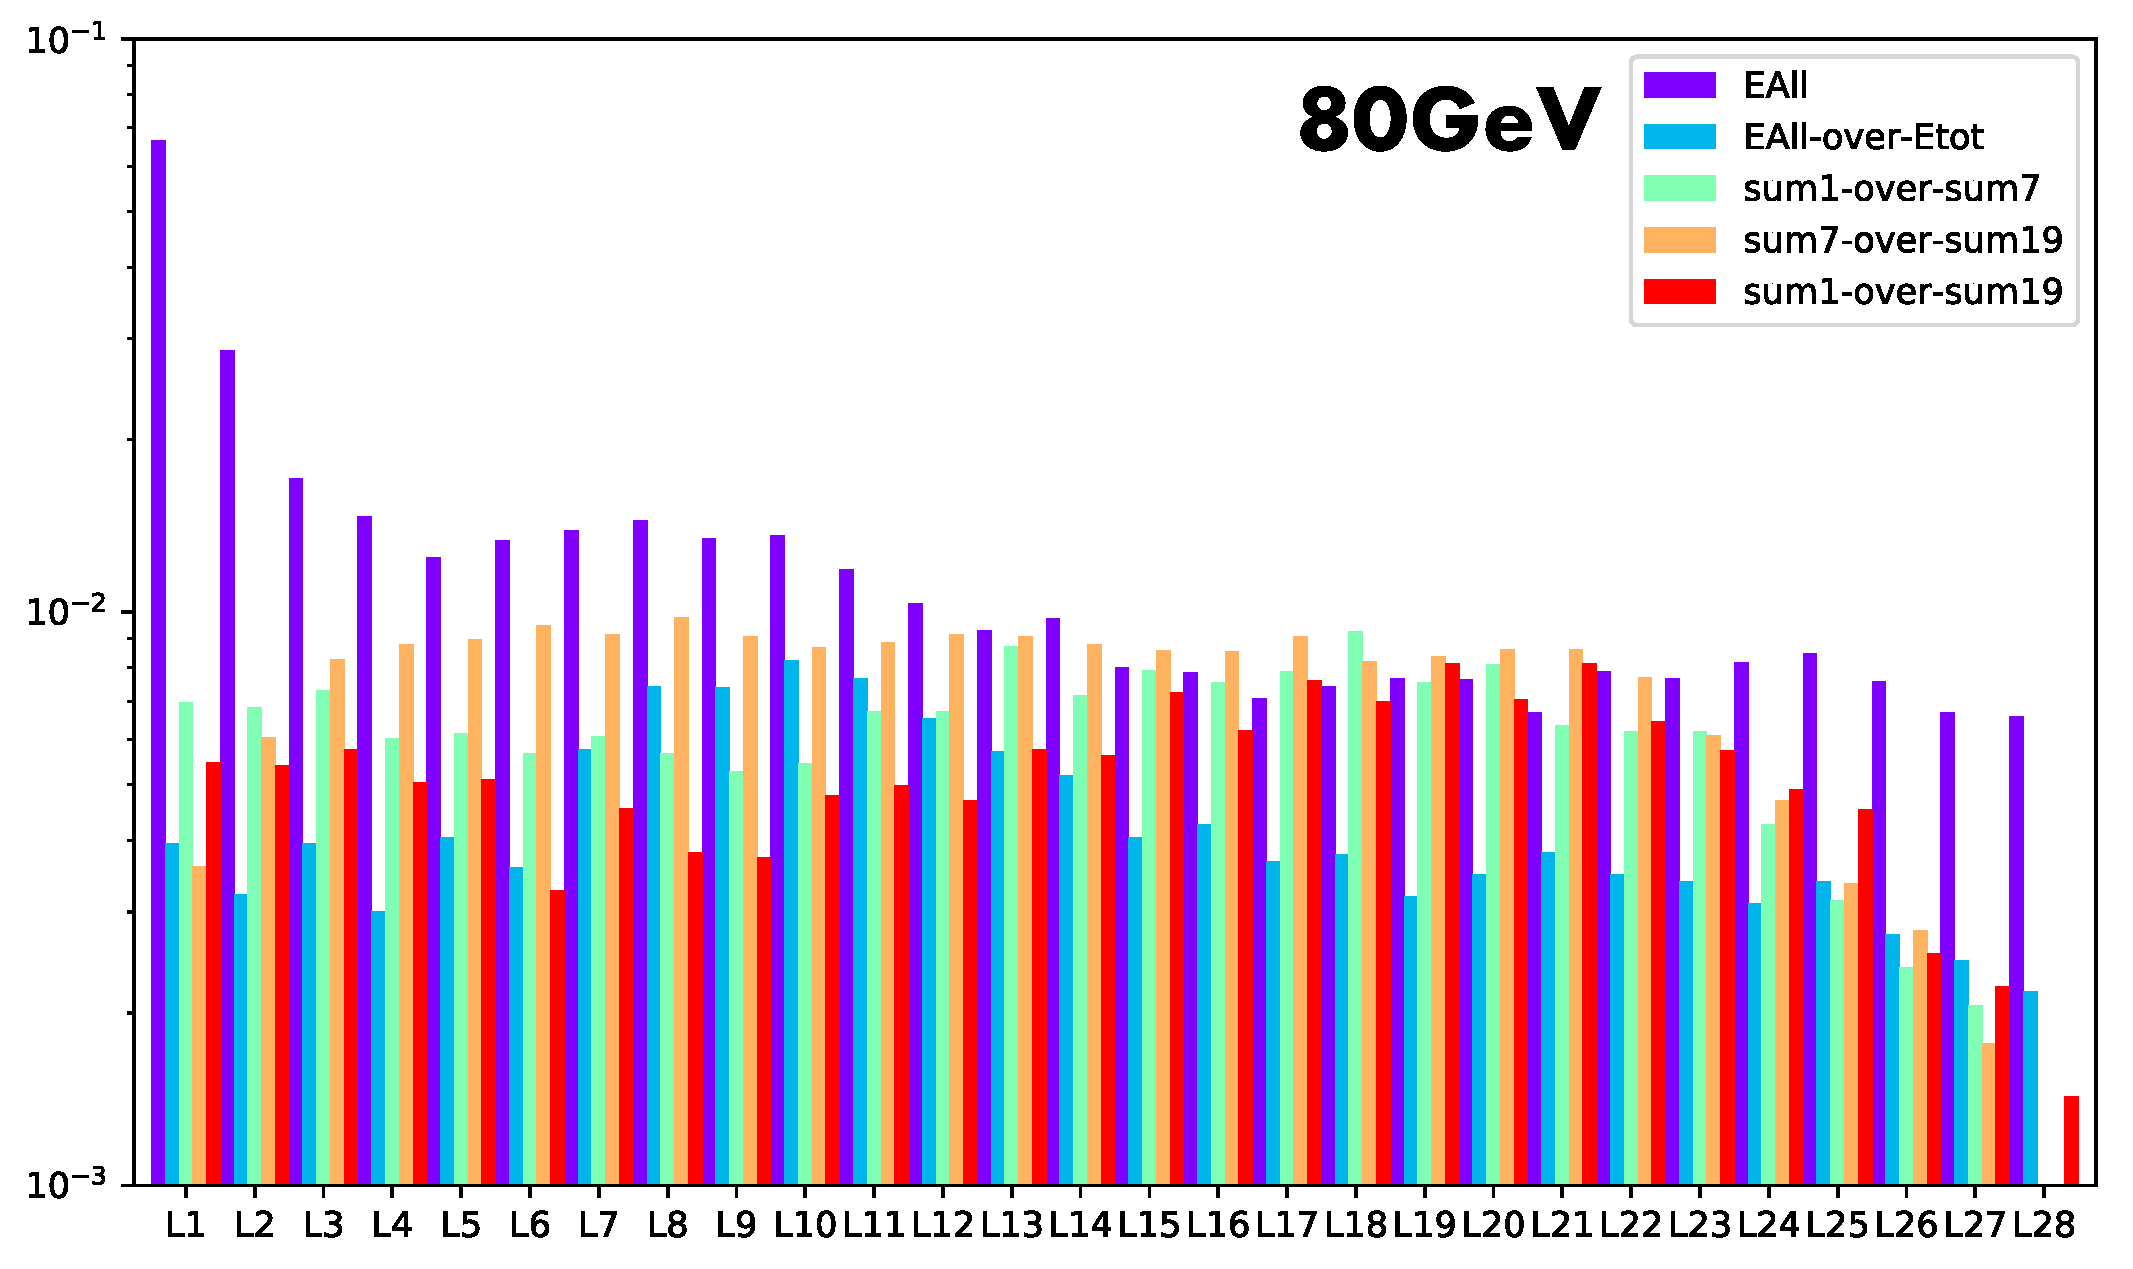
\includegraphics[width=0.5\textwidth]{Fig/fig_HGCAL/Feature_importance_showershape_dynamicwindow_v2_80GeV}~
    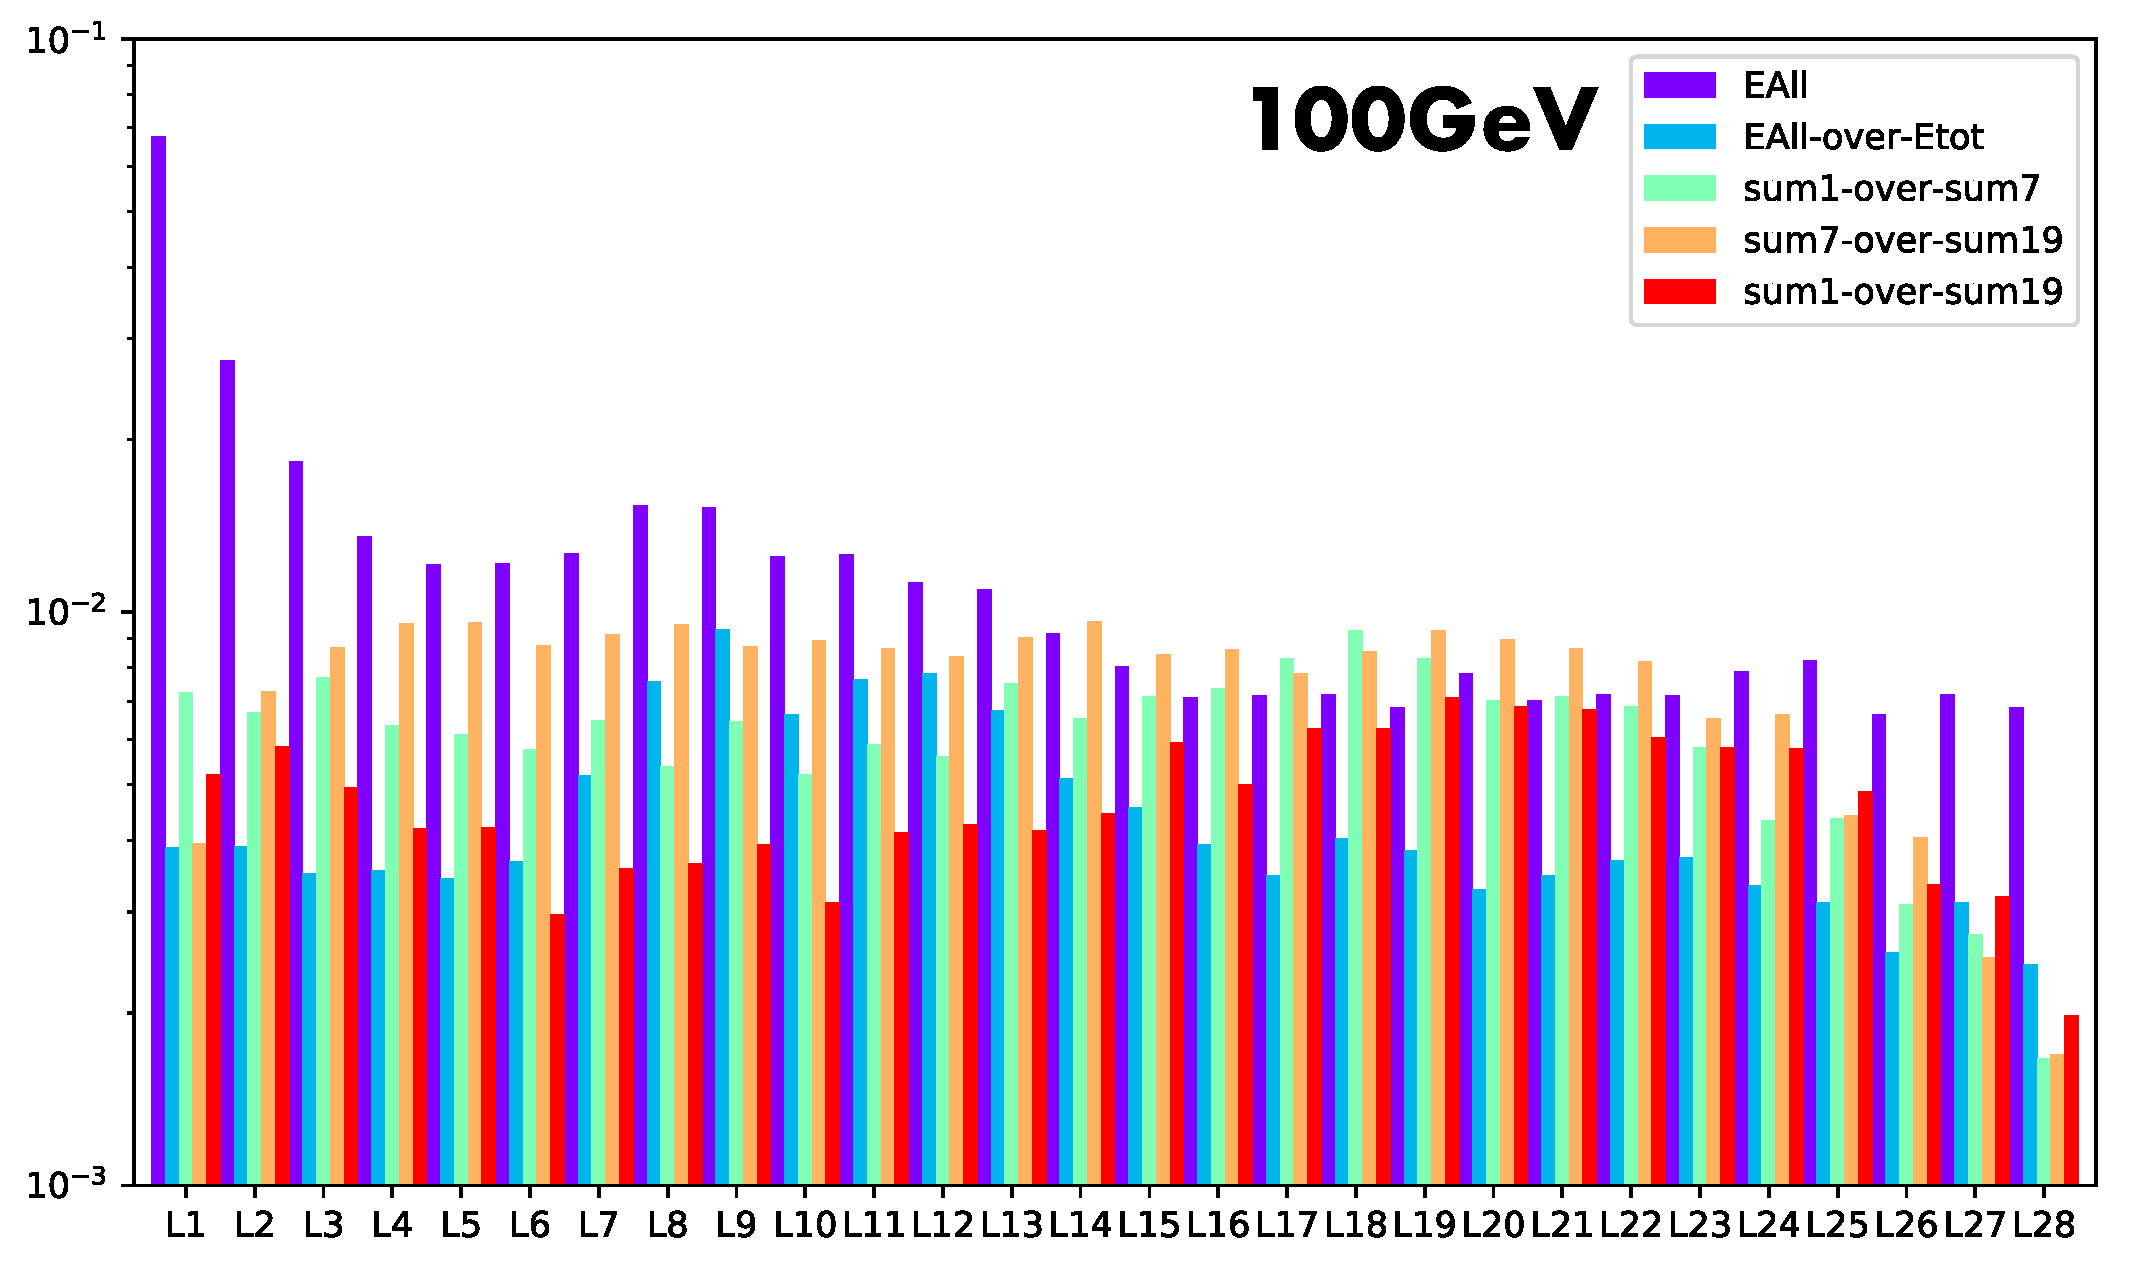
\includegraphics[width=0.5\textwidth]{Fig/fig_HGCAL/Feature_importance_showershape_dynamicwindow_v2_100GeV}\\
    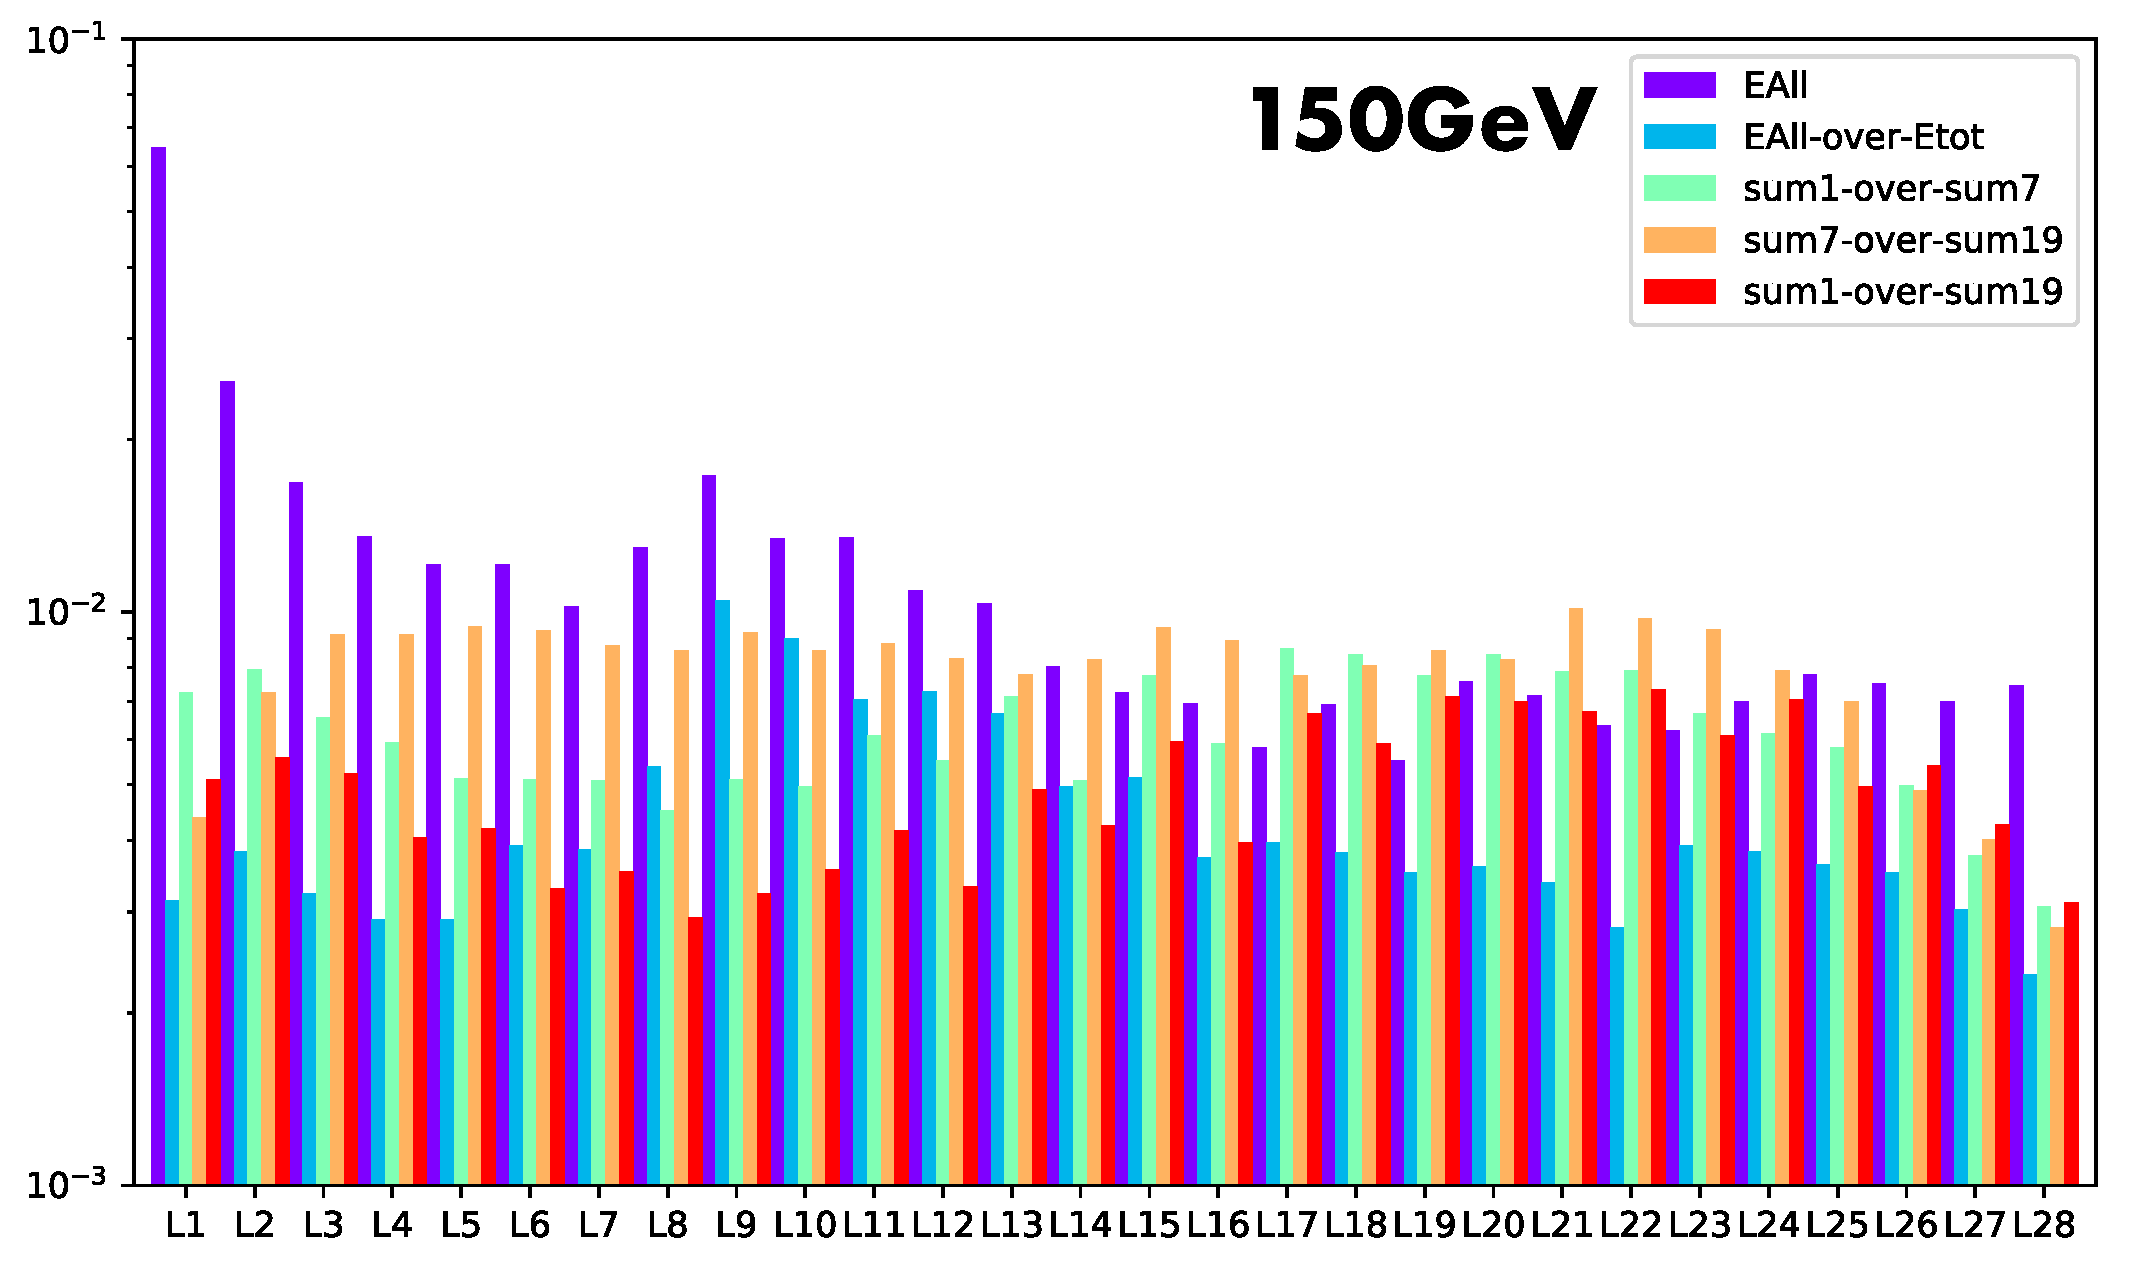
\includegraphics[width=0.5\textwidth]{Fig/fig_HGCAL/Feature_importance_showershape_dynamicwindow_v2_150GeV}~
    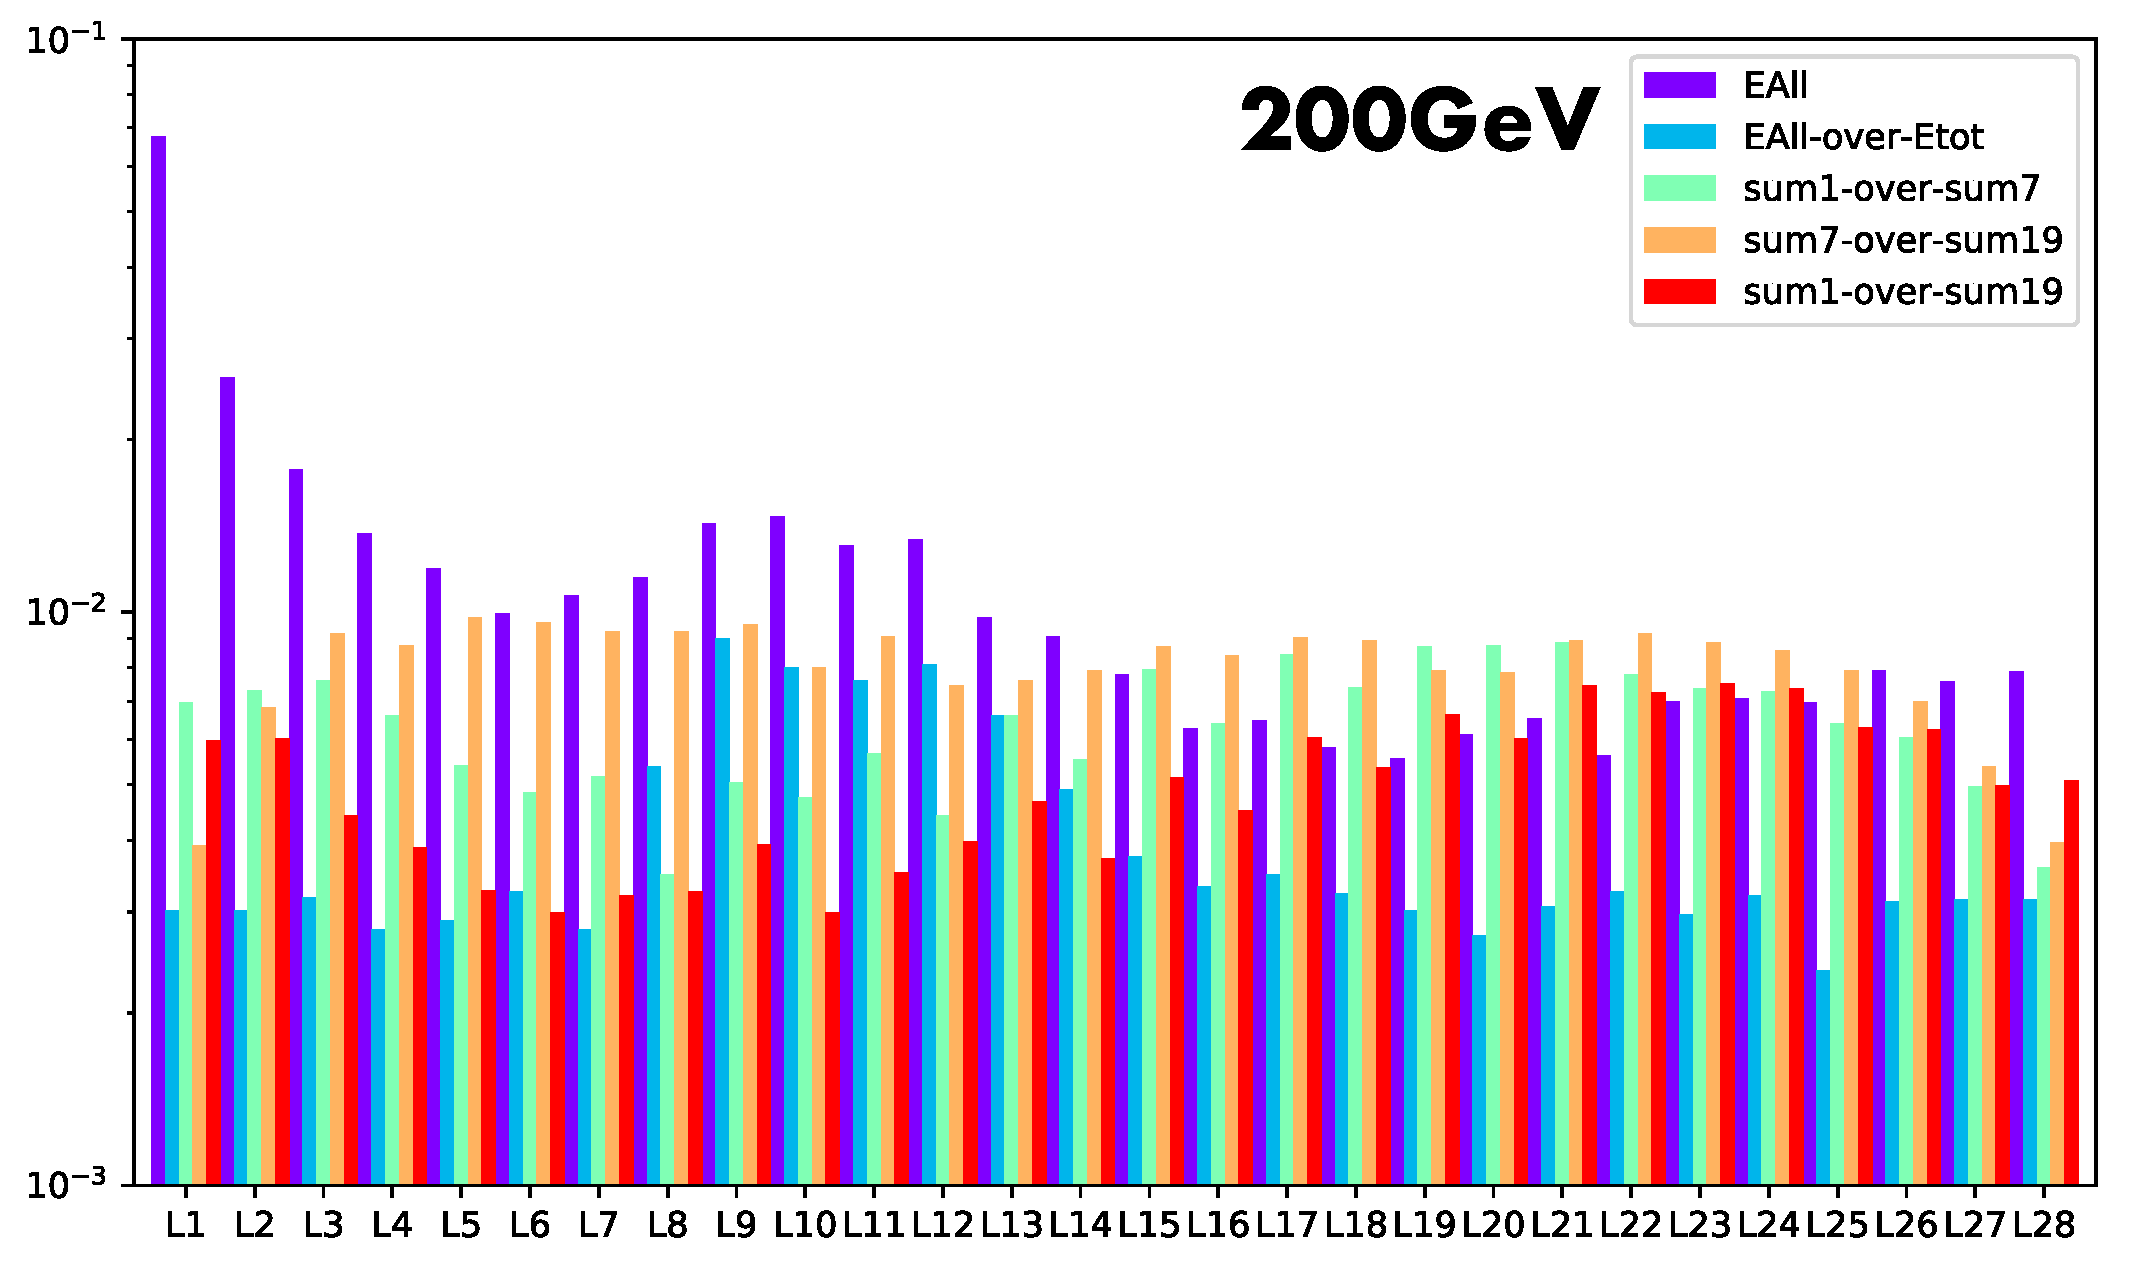
\includegraphics[width=0.5\textwidth]{Fig/fig_HGCAL/Feature_importance_showershape_dynamicwindow_v2_200GeV}\\
    \caption{Feature importances of the regression for all energy points.}
    \label{fig:featimp_EReco}
    \end{center}
\end{figure}

The full correlation matrix of the training features is shown in Fig.~\ref{fig:corr_matrix}.

\begin{figure}[p]
    \begin{center}  
    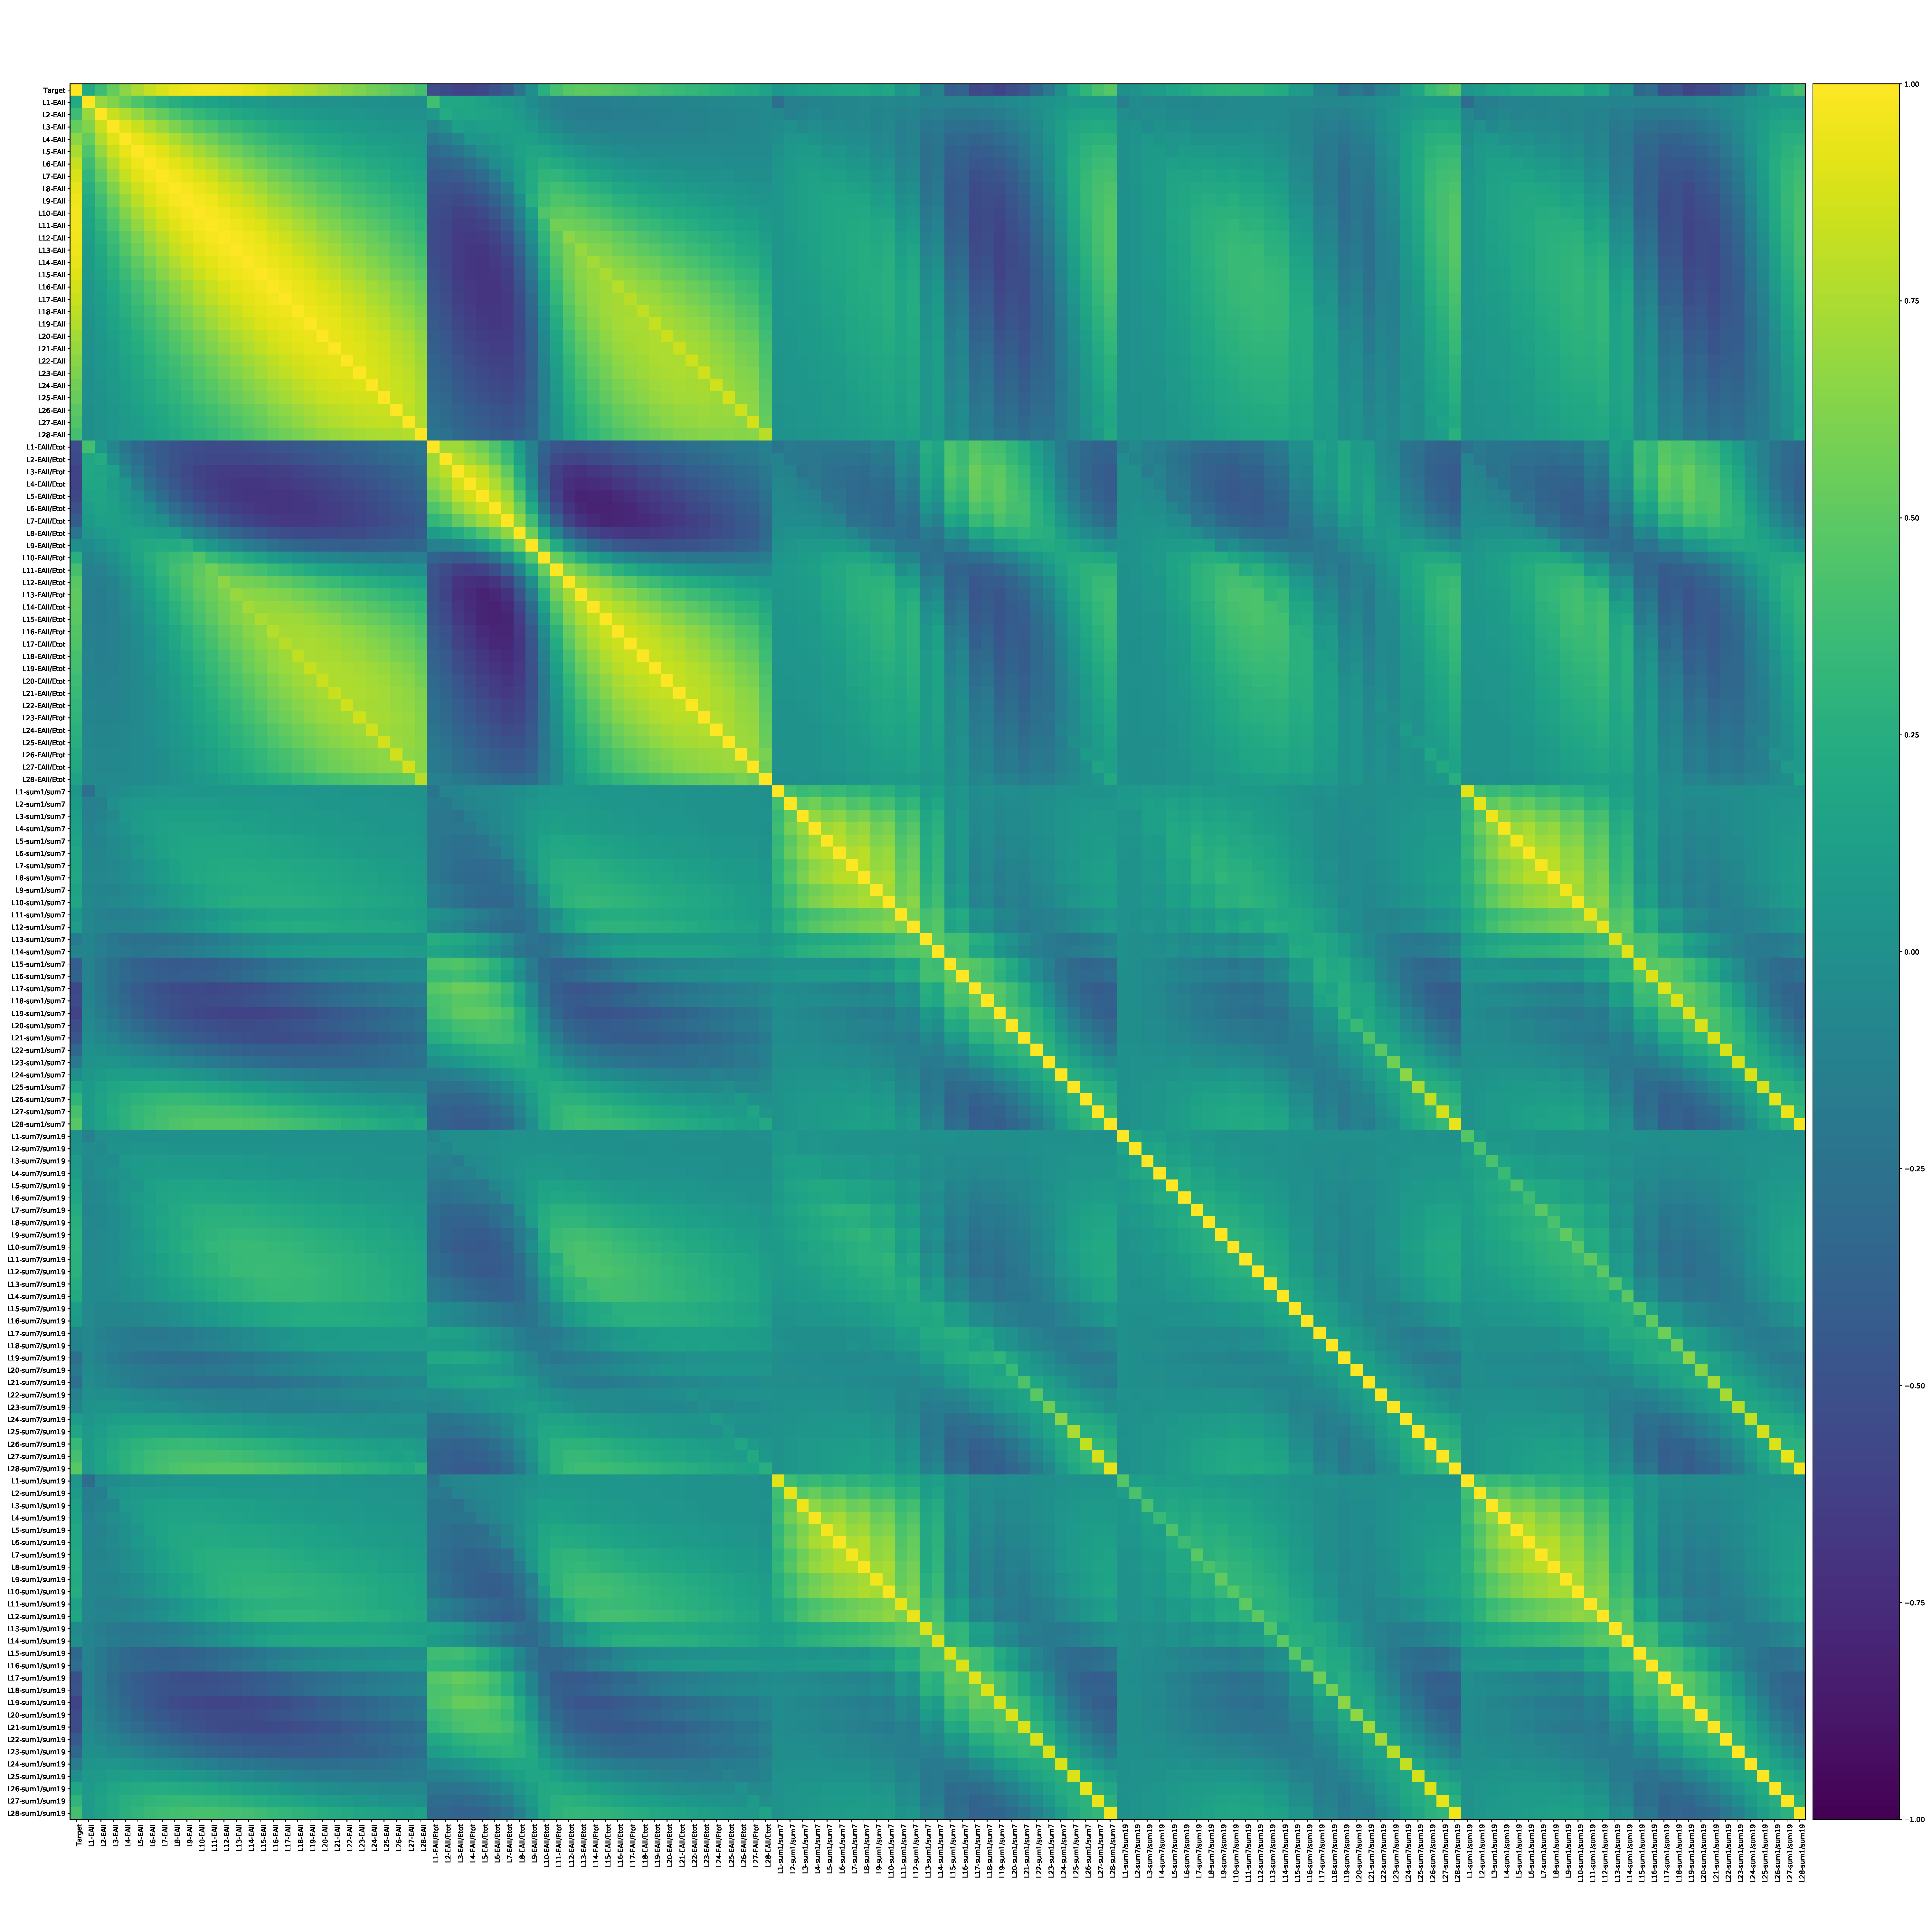
\includegraphics[width=1.0\textwidth]{Fig/fig_HGCAL/corr_matrix_showershape}\\
    \caption{The correlation matrix of the training features.}
    \label{fig:corr_matrix}
    \end{center}
\end{figure}


The latest results are shown in Fig.~\ref{fig:energyreco-bdt-latest}, where resolutions can be better than those from dEdx method when beam energy is greater than 50\GeV, yet for 20 and 30\GeV energy points the resolutions and energy responses are still worse than from dEdx method. The possible improvement is to add the shower depth information as the training features and see if the precision of the regression can be improved.

\begin{table}[!ht]
  \begin{center}
    {\small
    \begin{tabular}{lc}
    	Set &  (20, 30, 50, 60, 80, 100, 150, 200)\GeV \\
    	\hline
    	1 & ($\pm 8\GeV$, $\pm 8\GeV$, $\pm 8\GeV$, $\pm 8\GeV$, $\pm 8\GeV$, $\pm 8\GeV$, $\pm 10\GeV$, $\pm 10\GeV$) \\
    	2 & ($\pm 6\GeV$, $\pm 6\GeV$, $\pm 6\GeV$, $\pm 6\GeV$, $\pm 6\GeV$, $\pm 8\GeV$, $\pm 10\GeV$, $\pm 10\GeV$) \\
    \end{tabular}
    }
  \end{center}
  \caption{The sizes of dynamic energy window used in two different sets of regression.  \label{tab:EnergyWindowSize}}
\end{table}

\begin{figure}[!ht]
    \begin{center}  
    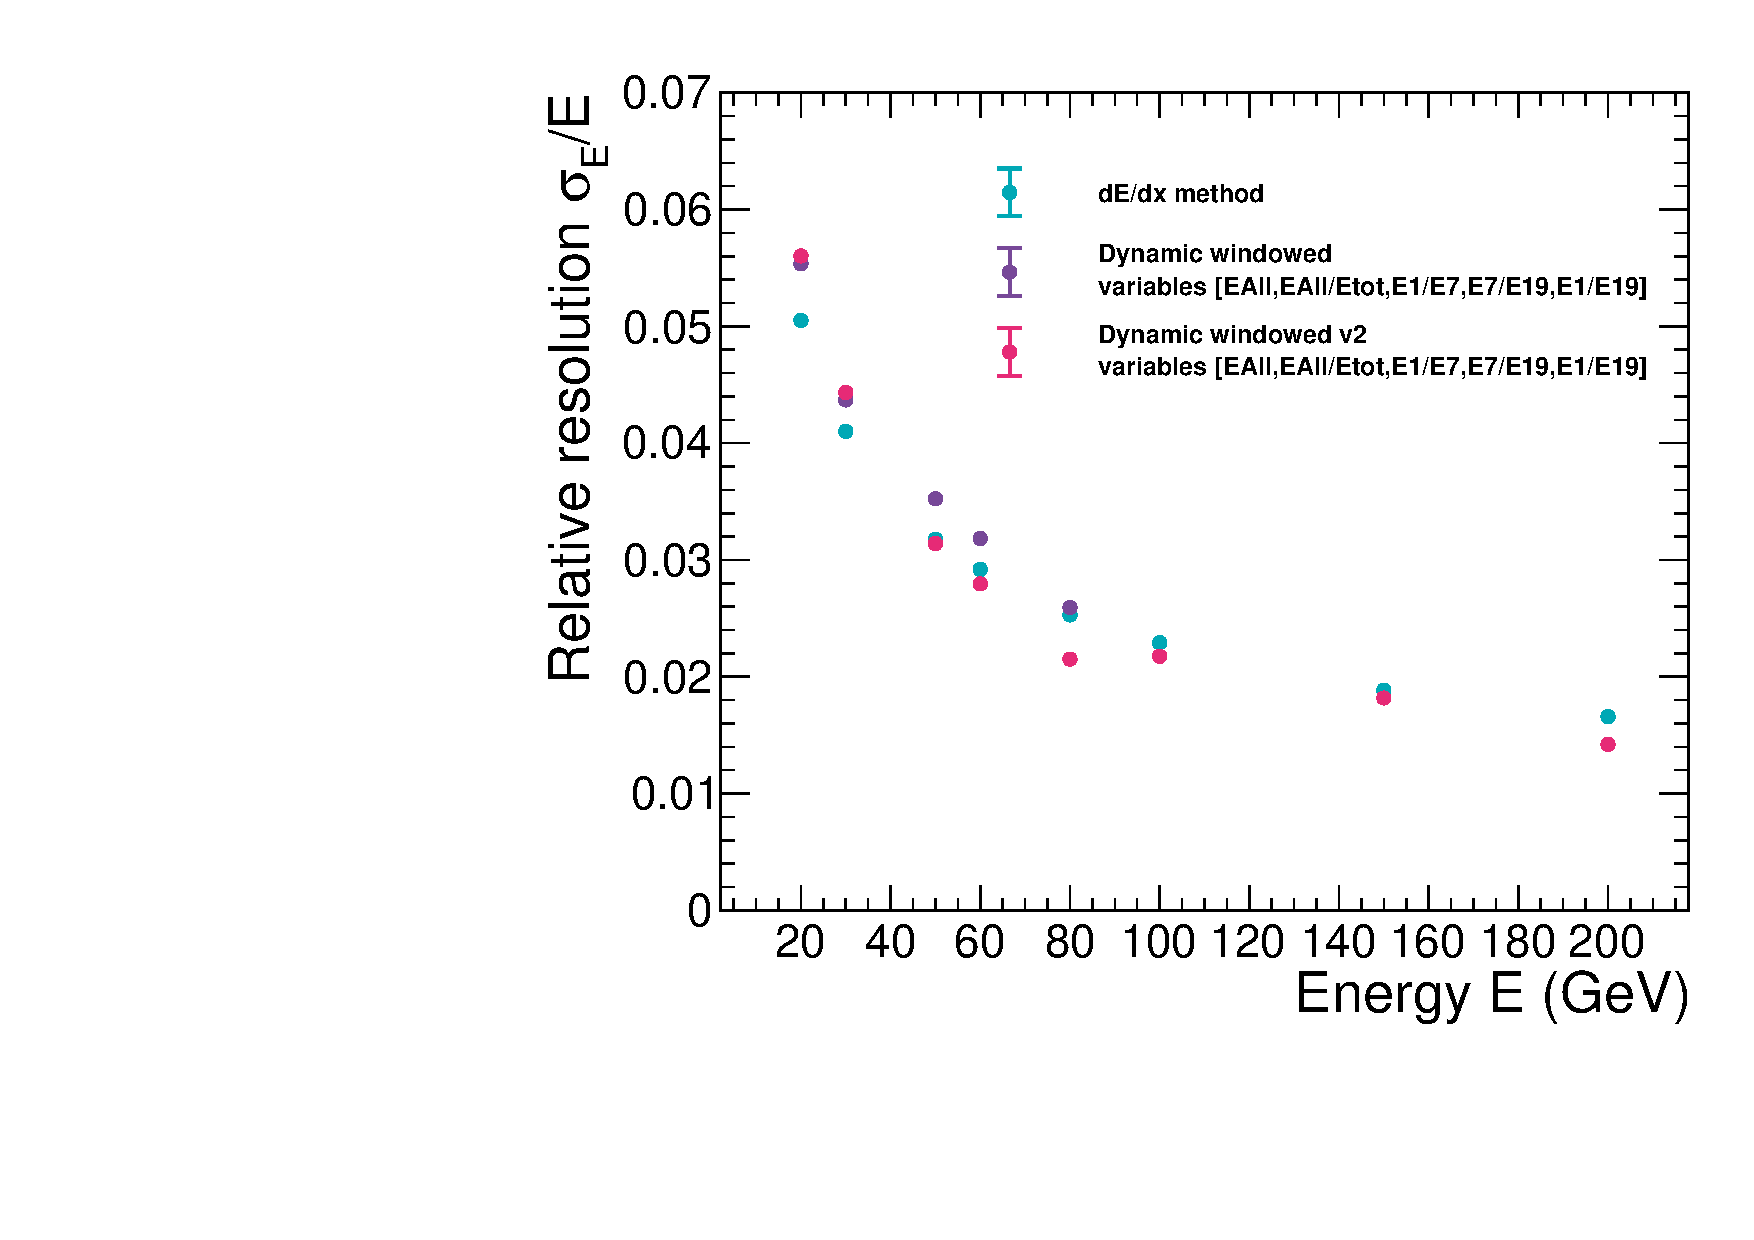
\includegraphics[width=0.5\textwidth]{Fig/fig_HGCAL/RelReso_comparison_dynamicwindow_showershape_v2}~
    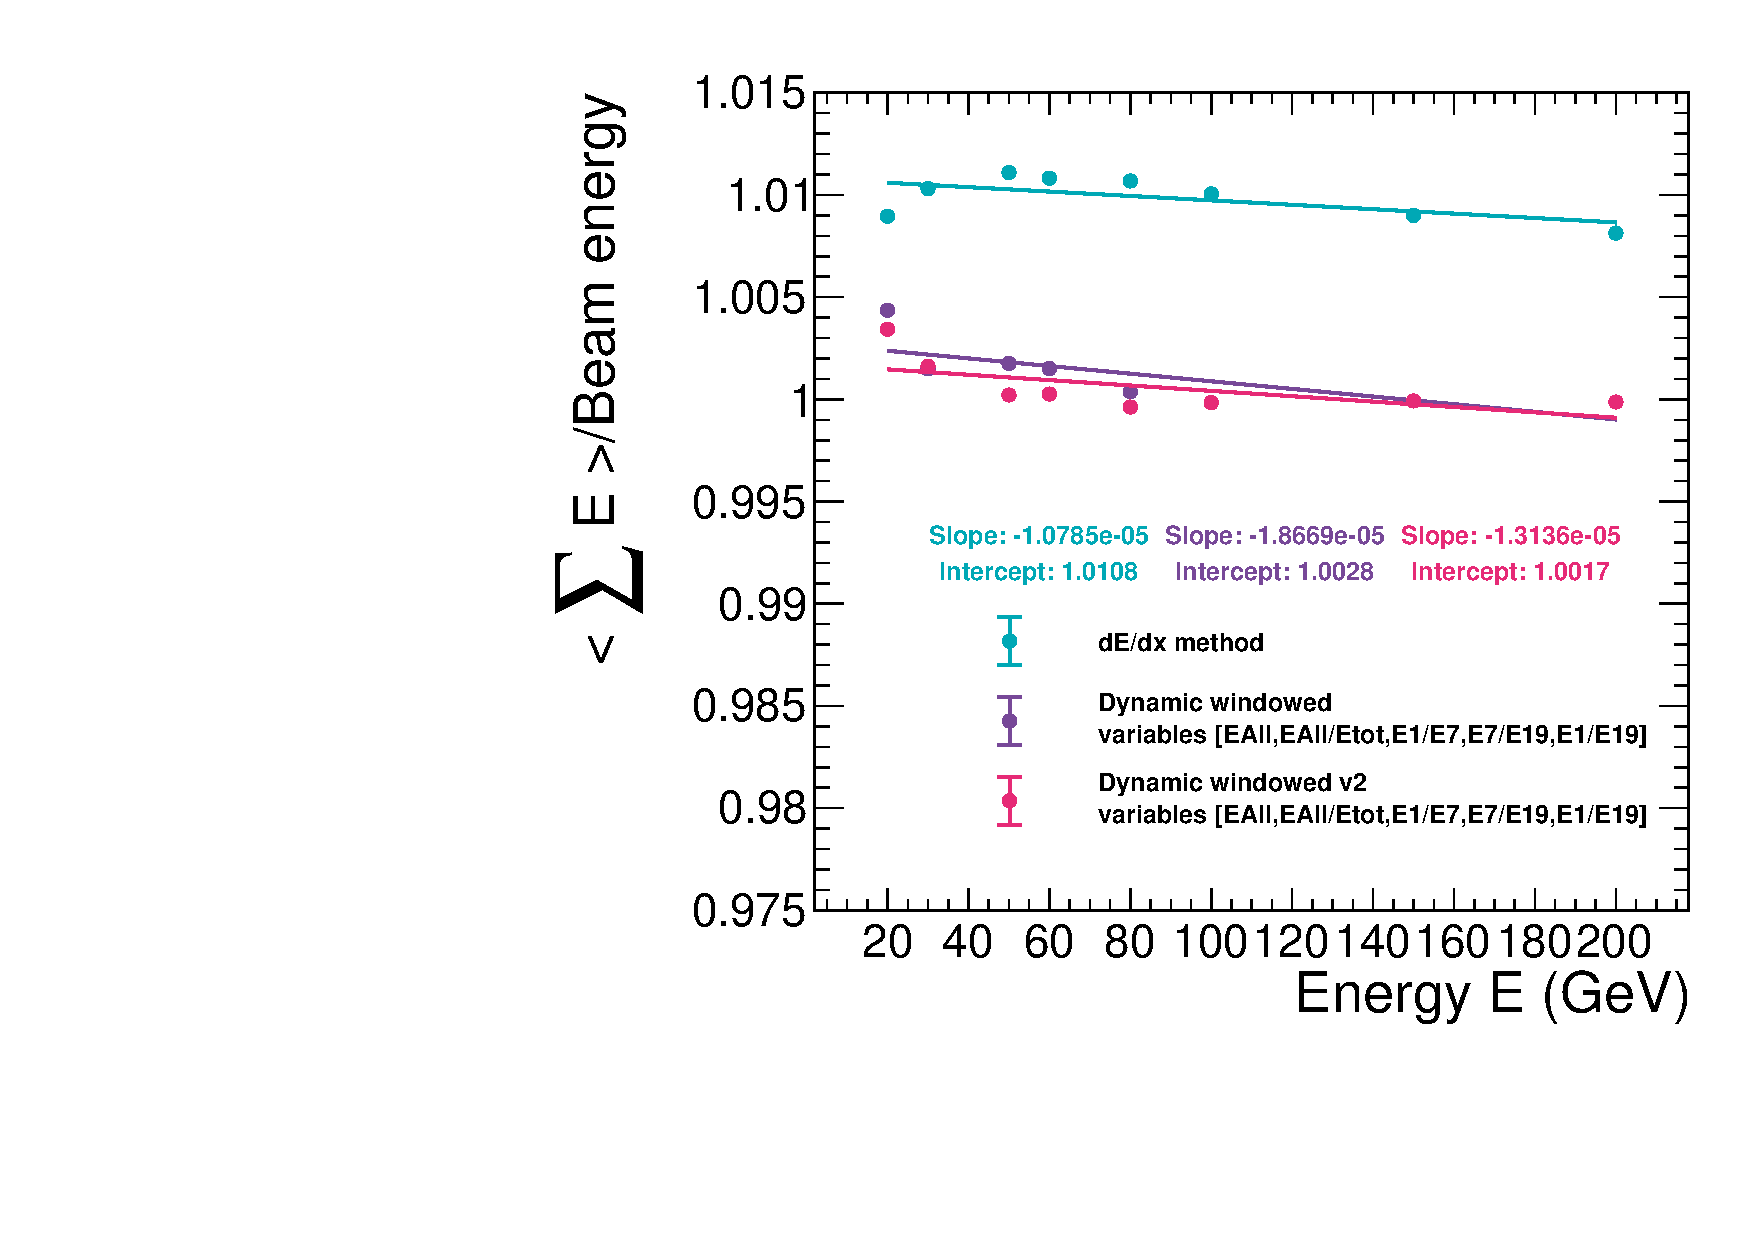
\includegraphics[width=0.5\textwidth]{Fig/fig_HGCAL/Response_comparison_dynamicwindow_showershape_v2}\\
    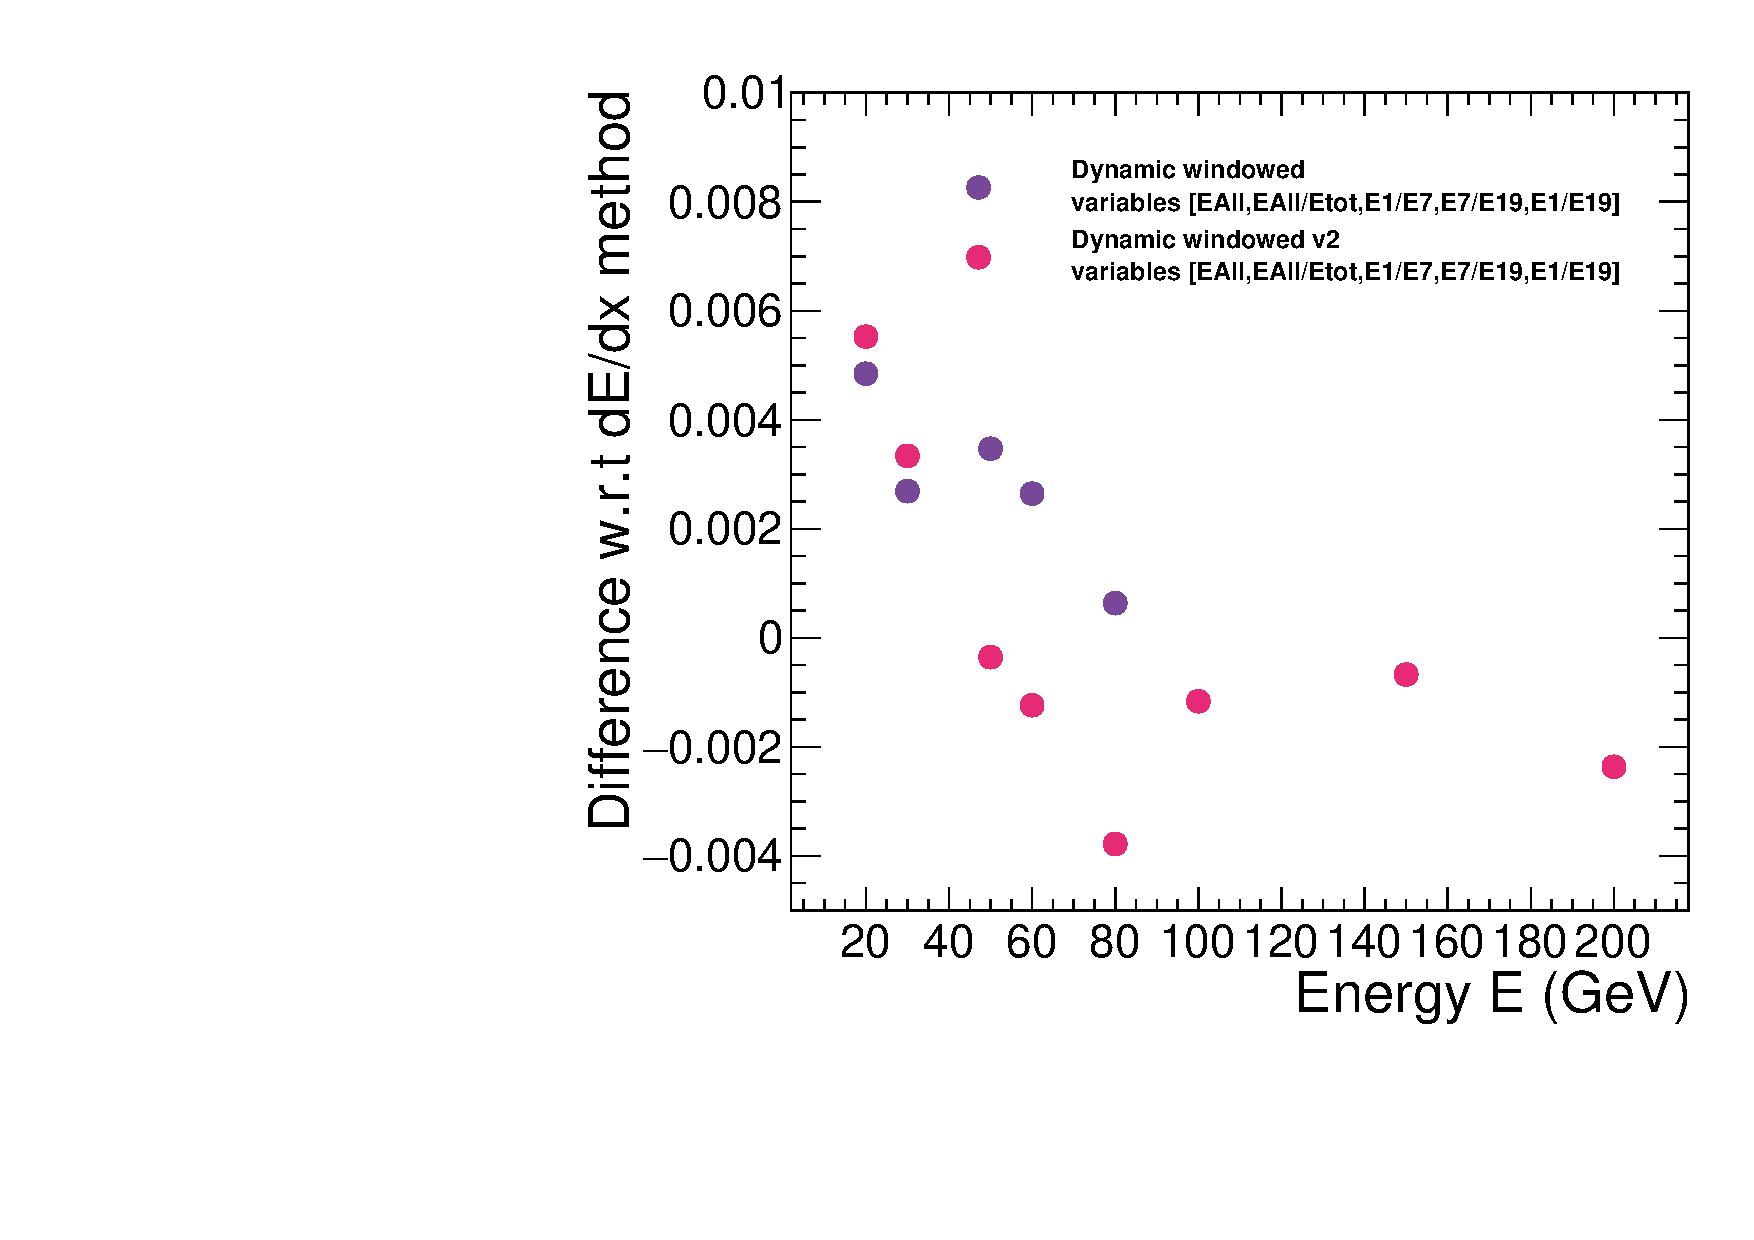
\includegraphics[width=0.5\textwidth]{Fig/fig_HGCAL/Diff-wrt-dEdx-dynamicwindow_v2}\\
    \caption{Results of the relative resolution as a function of predicted beam energy from regression (top left), the energy response as a function of predicted beam energy (top right), and the differences in relative resolutions with respect to those from dEdx method, with lateral shower shape variables being used as training features and dynamic window.}
    \label{fig:energyreco-bdt-latest}
    \end{center}
\end{figure}

Since this regression result will be applied on the beamtest data eventually, it is important to ensure the agreement between data and simulation, for which one need to select electron samples in beamtest data as pure as possible.

In the next section, the first systematical way to separate electron and pion for the beamtest data will be introduced.

\section{Electron and pion separation}
\label{sec:Electron ID}
One of the issues in beamtest data is the pion contamination. From previous experience a suggested way to discriminate electron and pion is to look at the median value of the RecHit energy distribution and the energy-weighted longitudinal shower depth, defined as
\begin{equation}
  \text{Longitudinal shower depth} = \frac{\sum_{i=1}^{28}(\text{EAll}_{i}\times X_{0, i})}{\sum_{i=1}^{28} \text{EAll}_{i}}.
\end{equation}

Fig.~\ref{fig:pionContamination-scatter} shows an example of the scatter plot of the median value of the RecHit energy distribution (will be abbreviated as mdn of RecHit in the following text) and the energy-weighted longitudinal shower depth (will be abbreviated as depthX0 in the following text) from 100\GeV beamtest data and simulation samples, and for better visualization, 2-dimension histograms for all the three samples are also shown. It is obvious that the pure electron events distribute differently from pure pion events, and in the beamtest data there is pion contamination. 

\begin{figure}[!ht]
    \begin{center}  
    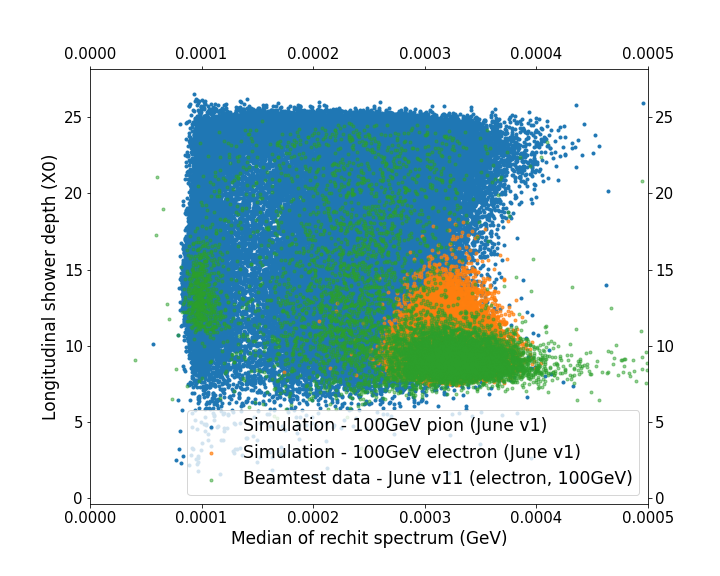
\includegraphics[width=0.7\textwidth]{Fig/fig_HGCAL/PionContamination_100GeV}\\
    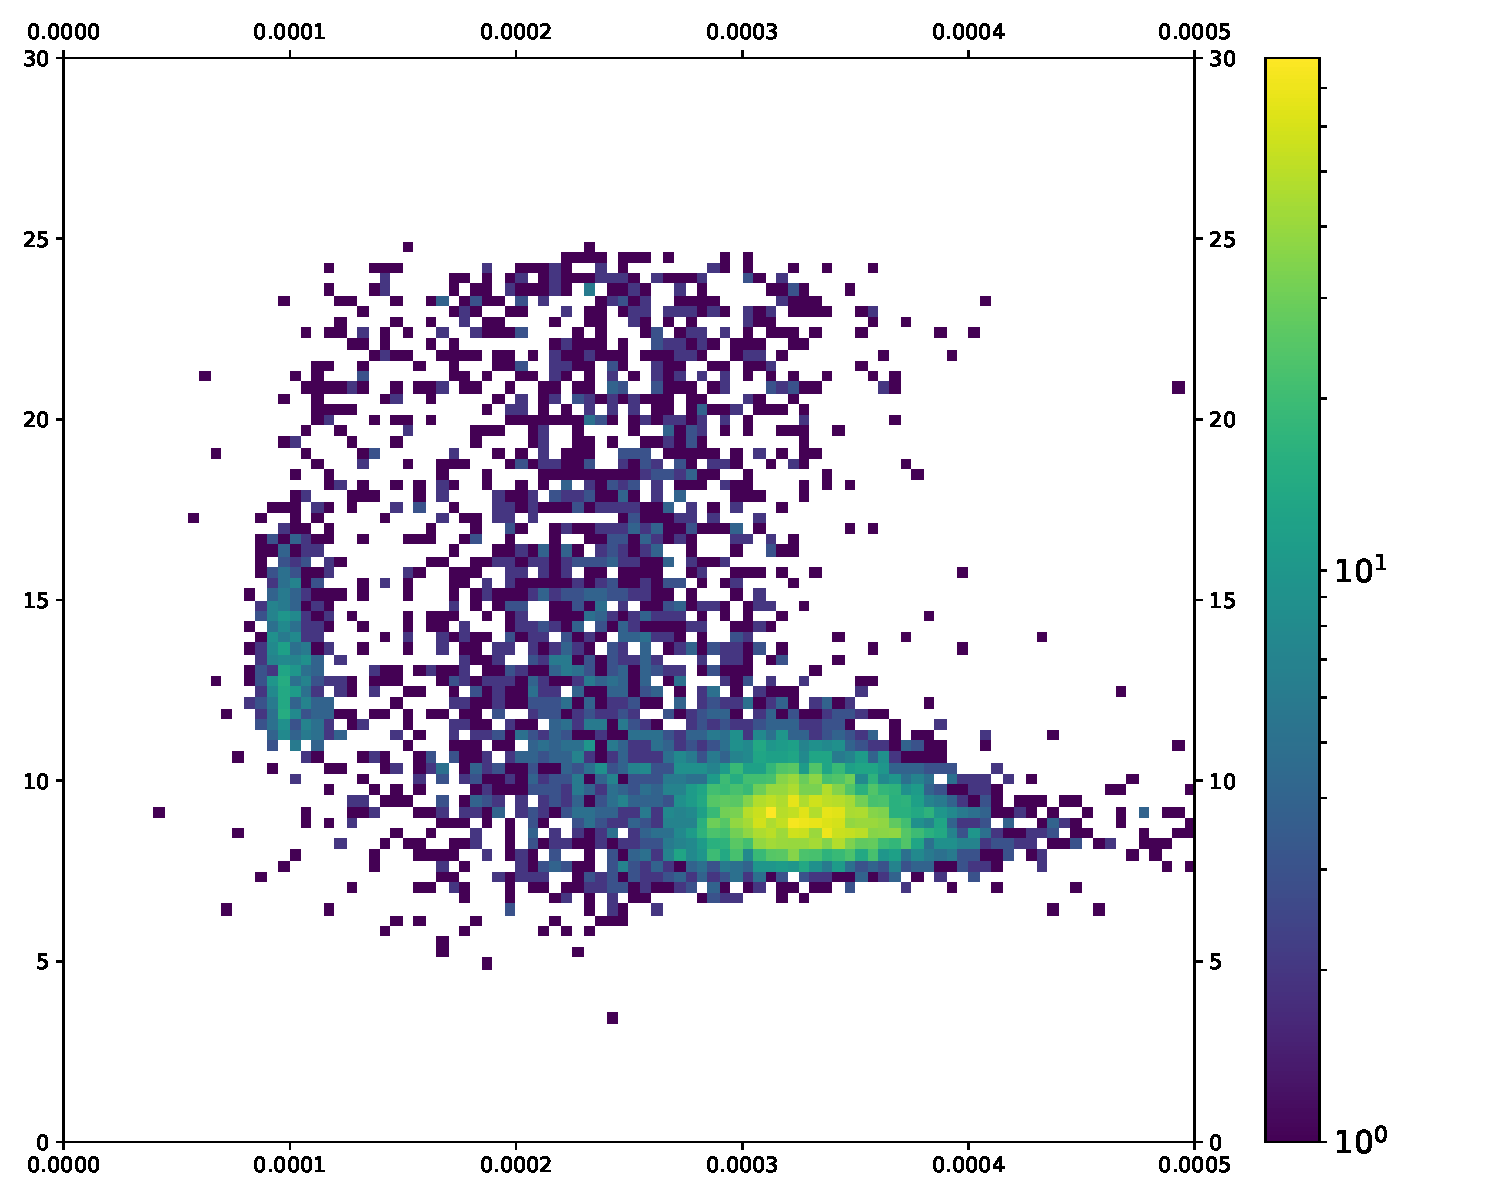
\includegraphics[width=0.33\textwidth]{Fig/fig_HGCAL/DataJunev11_Run240_100GeV_WithoutCuts}~
    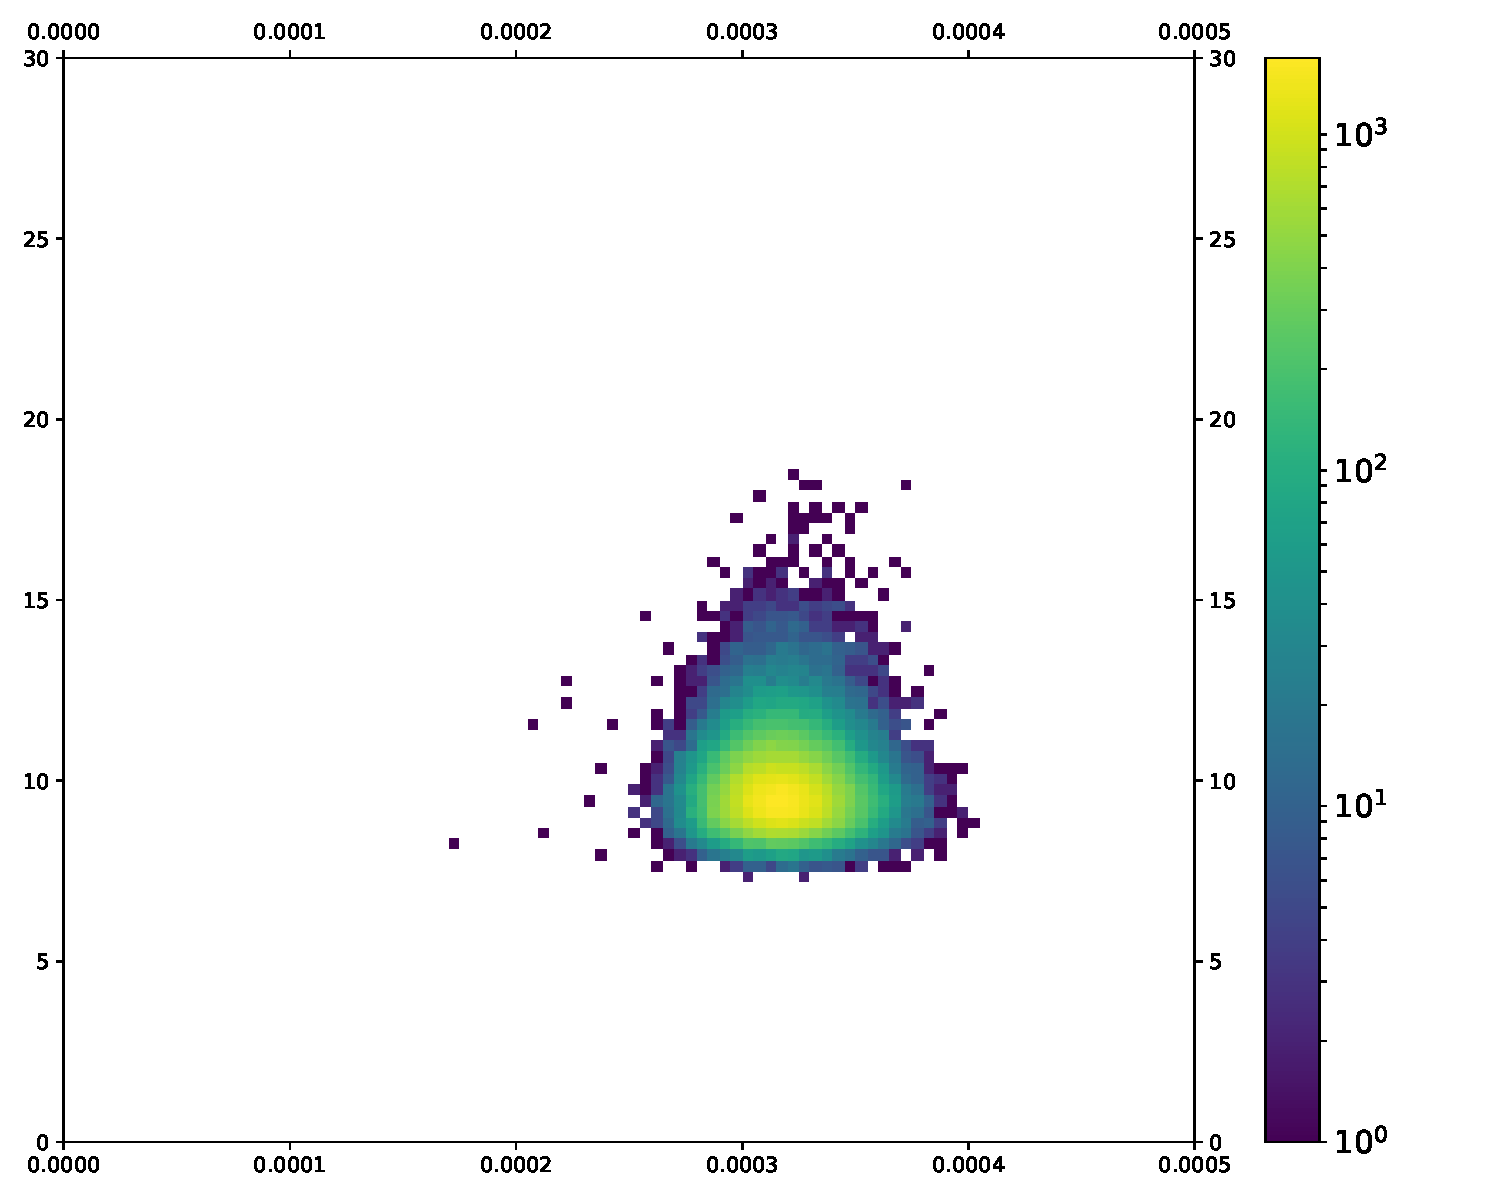
\includegraphics[width=0.33\textwidth]{Fig/fig_HGCAL/Electron_Junev1_100GeV_WithoutCuts}~
    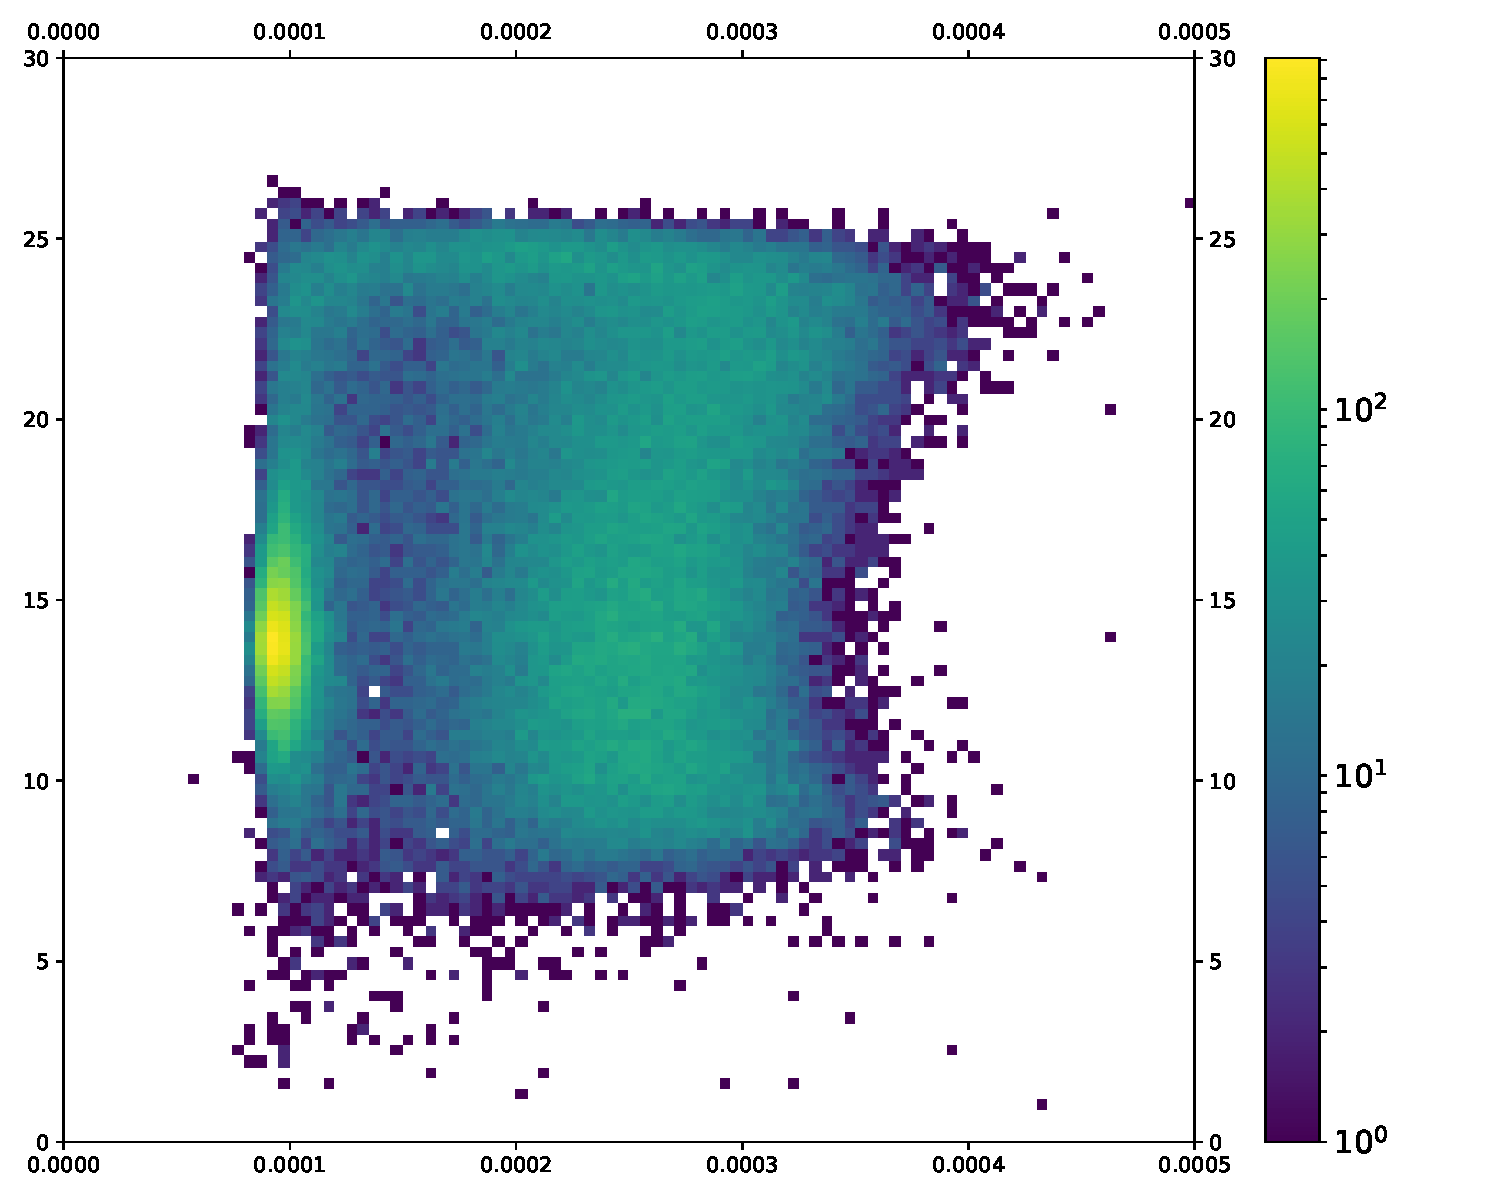
\includegraphics[width=0.33\textwidth]{Fig/fig_HGCAL/Pion_Junev1_100GeV_WithoutCuts}\\
    \caption{The scatter plot of the median value of the RecHit energy distribution and the energy-weighted shower depth from 100\GeV beamtest data and simulation samples (top); 2-dimension histograms for beamtest data (bottom left), electron simulation (bottom middle), and pion simulation (bottom right). }
    \label{fig:pionContamination-scatter}
    \end{center}
\end{figure}

The simplest way to reject pion events is to impose a straight line, and identify the events on the right hand side of it as electrons. However, it is difficult to choose a proper slope and intersection systematically.
Alternatively, a "2-dimension window" cut is proposed. The basic ideas are:
\begin{itemize}  
\item To construct a 2-D window that contains a fraction $N\%$ of electron events, $\sqrt{N}\%$ of events should be contained in each dimension (i.e.,  mdn of RecHit or depthX0).
\item From the 1-dimension distributions of mdn of RecHit (depthX0) in certain range of depthX0 (mdn of RecHit), one can obtain $\sqrt{N}\%$ quantile of the distribution. Examples of the 1-dimension distributions can be found in Fig.~\ref{fig:1DHist-quantile}, where the lines with different colors indicate the starting and ending points of certain quantile.
\item By scanning over the range where there are enough statistics, one can obtain all the starting and ending points of the quantiles of the distributions over the scanned range. The left plot of Fig.~\ref{fig:2DHist-quantile} shows an example. Here one can already see the outline of the window.
\item By fitting all the starting and ending points for given quantile with straight line (polynomial of order one), one obtains functions that roughly describe the relation between the mdn of RecHit and depthX0. The right plot of Fig.~\ref{fig:2DHist-quantile} shows the fit results. The events inside the quadrangles are then identified as electron events, where different sizes represent the "2-dimension window" cut with different signal efficiencies (working points).
\end{itemize}

Fig.~\ref{fig:2DHist-Window-Data-pion} shows the "2-dimension window" cut applied on beamtest data and pion simulation samples. The electron (signal) efficiency as a function of the pion (background) efficiency is shown in the left plot of Fig.~\ref{fig:Window-WP}, while the electron (signal) efficiencies as a function of background rejection power, defined as the reciprocal of background efficiency, is in the right plot. One can see that the actual signal efficiencies are close to the desired working points. The efficiencies in beamtest data, defined as the ratio of the number of events retained in the window cut over total number of events in the sample, are listed in Table.~\ref{tab:Window-EffData}.

\begin{table}[!ht]
  \begin{center}
    {
    \begin{tabular}{cc}
    	WP (\%) &  Efficiency in beamtest data (\%) \\
    	\hline
    	68.3 & 19.4 \\
    	80.0 & 25.0 \\
    	90.0 & 30.9 \\
    	95.0 & 35.7 \\
    	99.0 & 42.5 \\
    \end{tabular}
    }
  \end{center}
  \caption{The efficiencies in beamtest data with different working points.  \label{tab:Window-EffData}}
\end{table}

\begin{figure}[!ht]
    \begin{center}  
    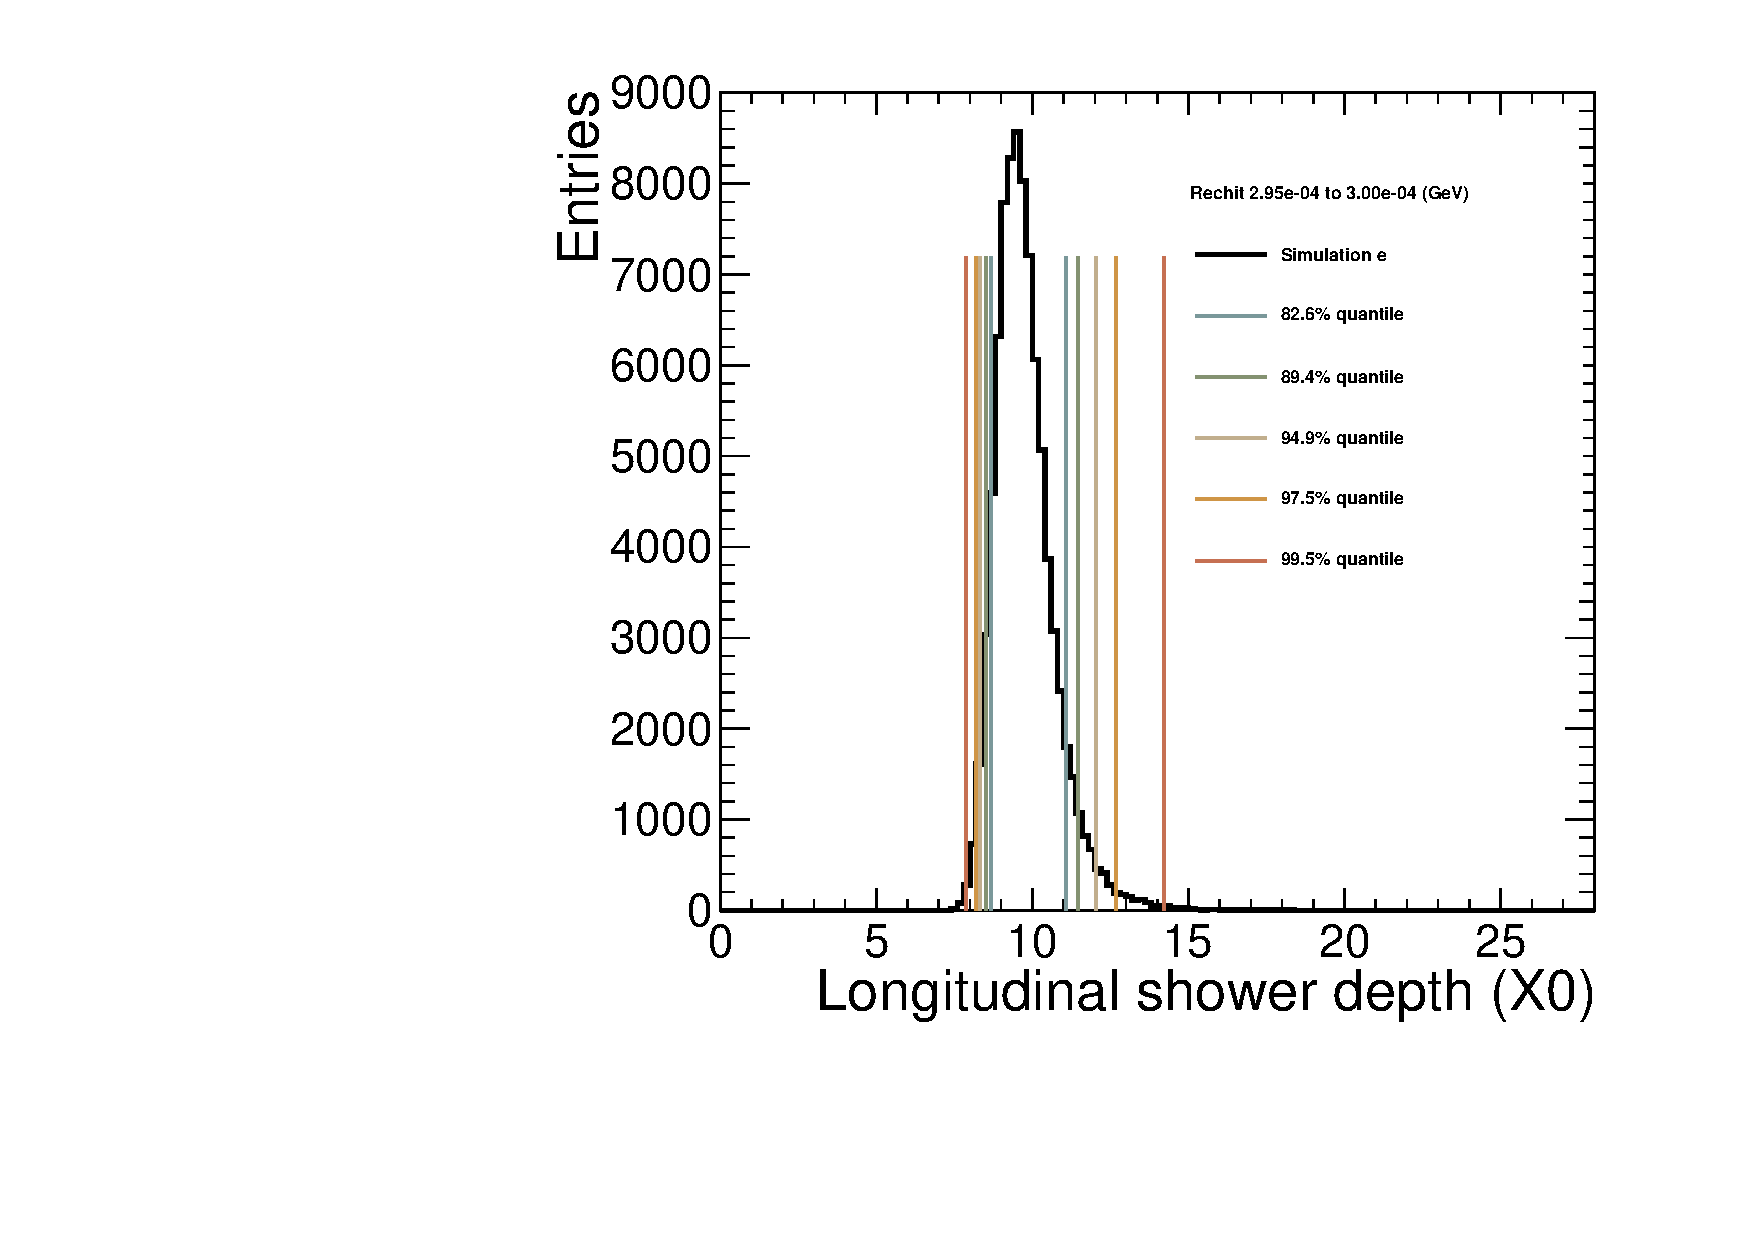
\includegraphics[width=0.5\textwidth]{Fig/fig_HGCAL/depthX0-Rechit2p95e-04to3p00e-04}~
    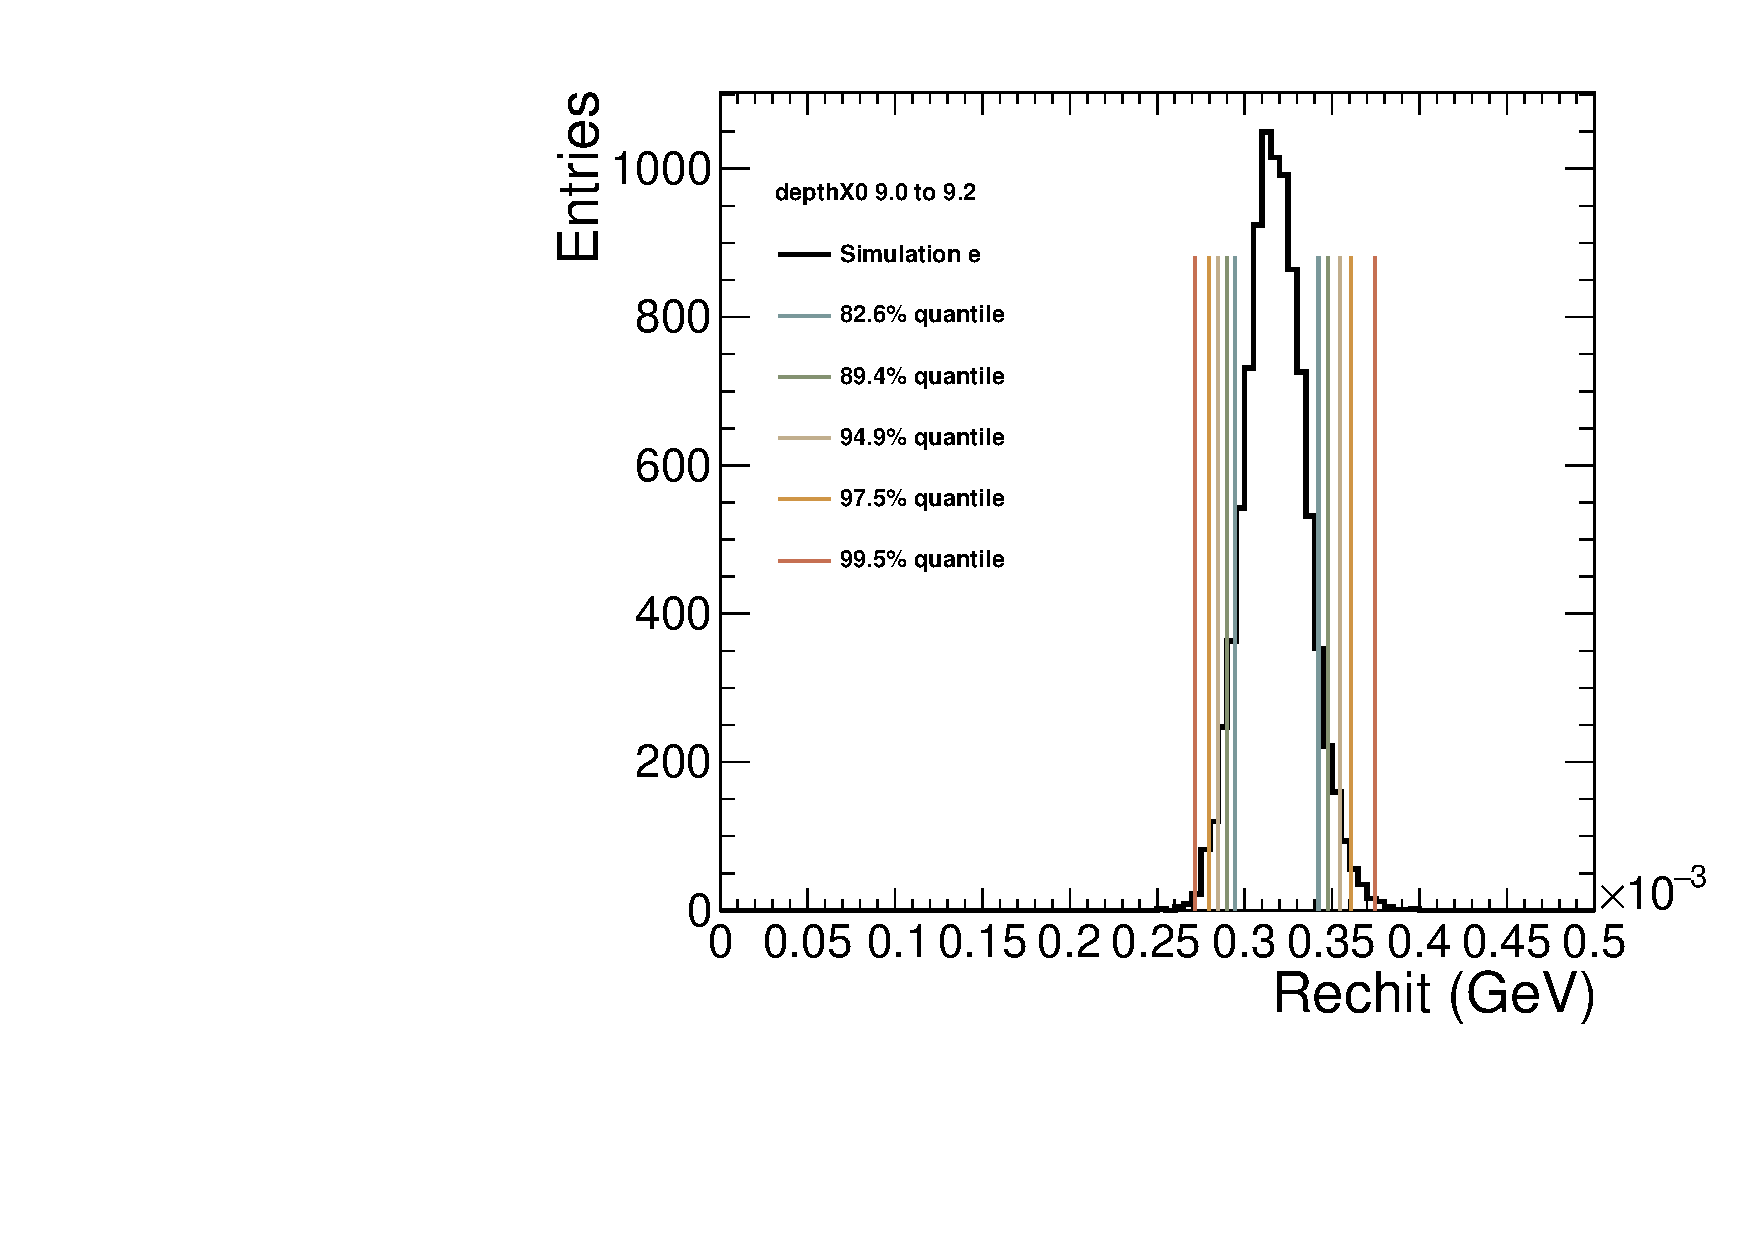
\includegraphics[width=0.5\textwidth]{Fig/fig_HGCAL/Rechit-depthX09p0to9p2}\\
    \caption{1-dimension distributions of mdn of RecHit (depthX0) in certain range of depthX0 (mdn of RecHit), with different quantiles (labeled in legend).}
    \label{fig:1DHist-quantile}
    \end{center}
\end{figure}

\begin{figure}[!ht]
    \begin{center}  
    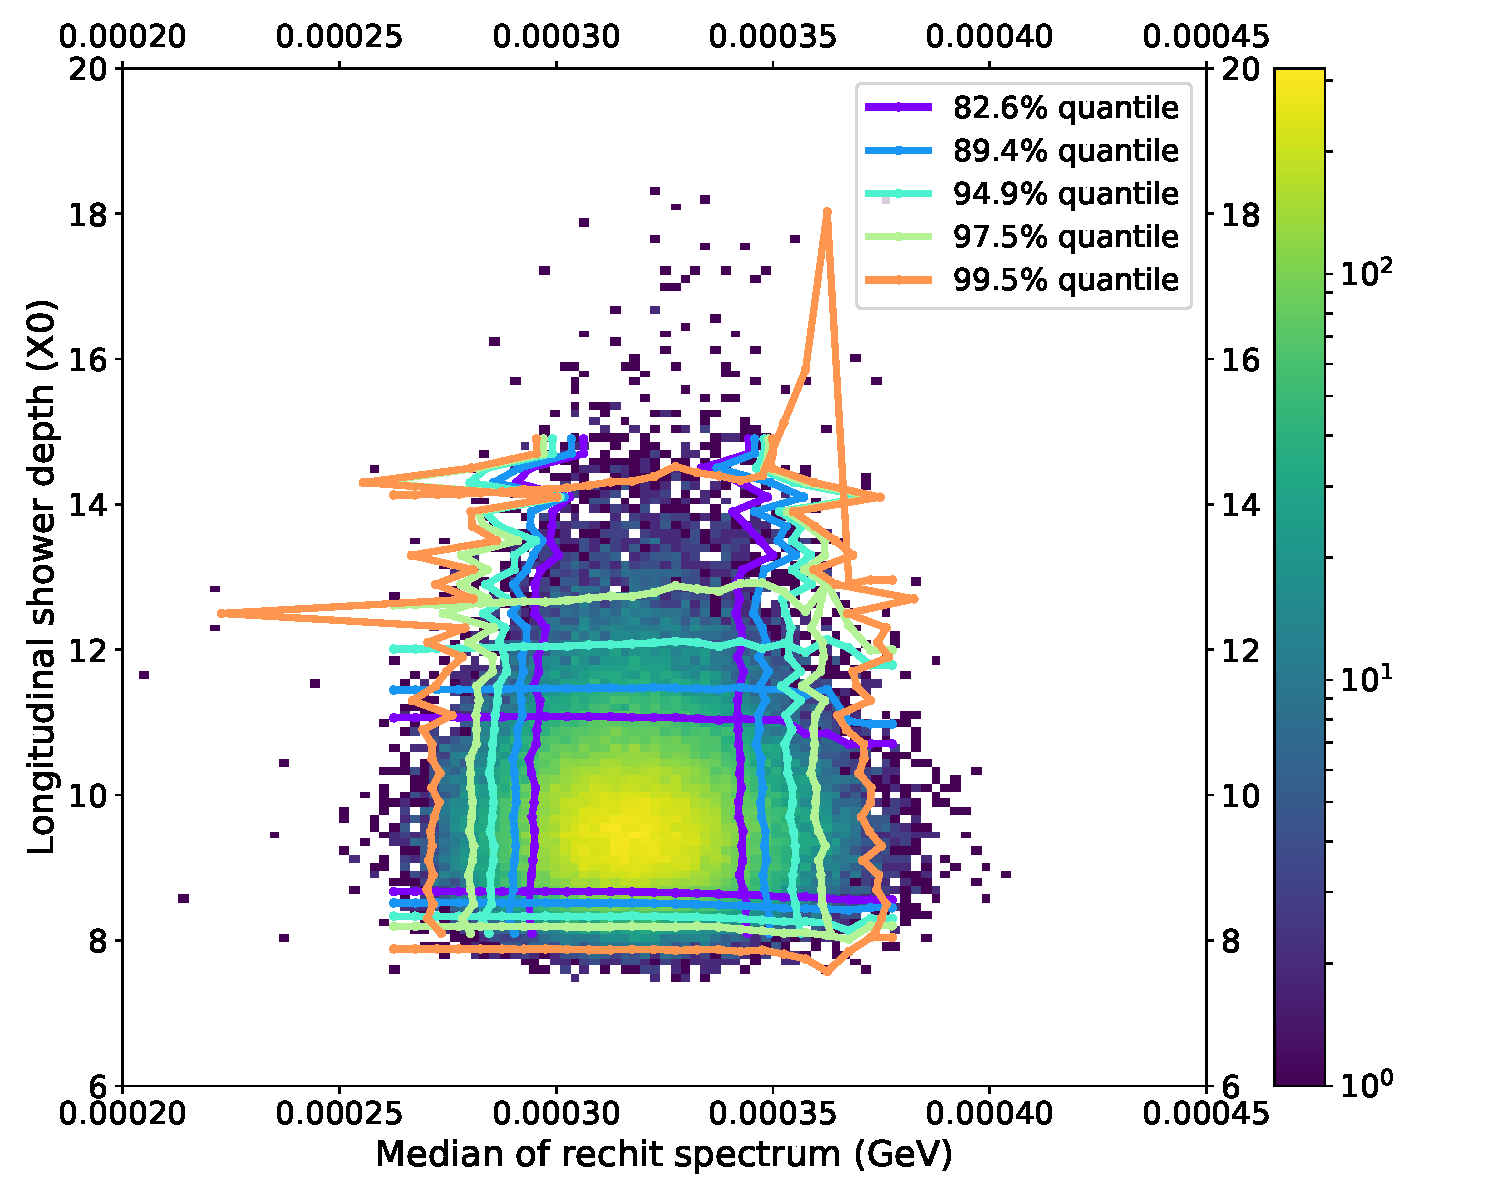
\includegraphics[width=0.5\textwidth]{Fig/fig_HGCAL/Electron-Quantile-100GeV}~
    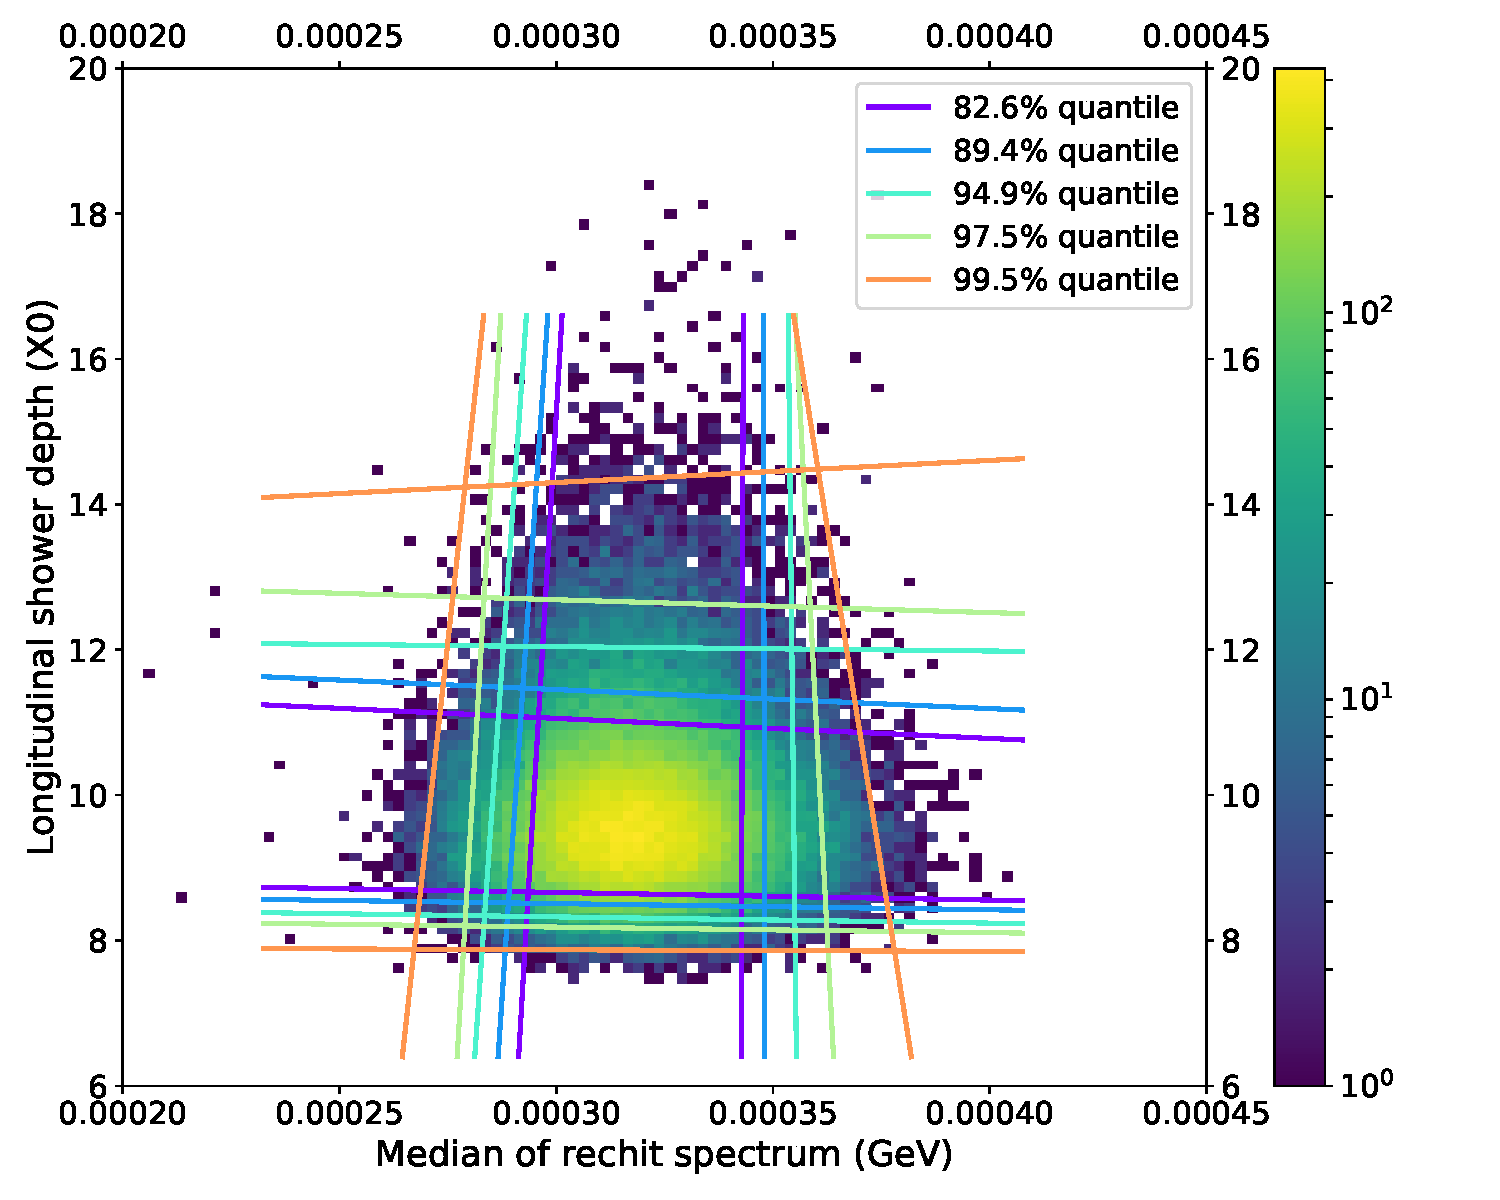
\includegraphics[width=0.5\textwidth]{Fig/fig_HGCAL/Electron-Quantile-FitResults-100GeV}\\
    \caption{The starting and ending points of the quantiles over the range where there are enough statistics.}
    \label{fig:2DHist-quantile}
    \end{center}
\end{figure}

\begin{figure}[!ht]
    \begin{center}  
    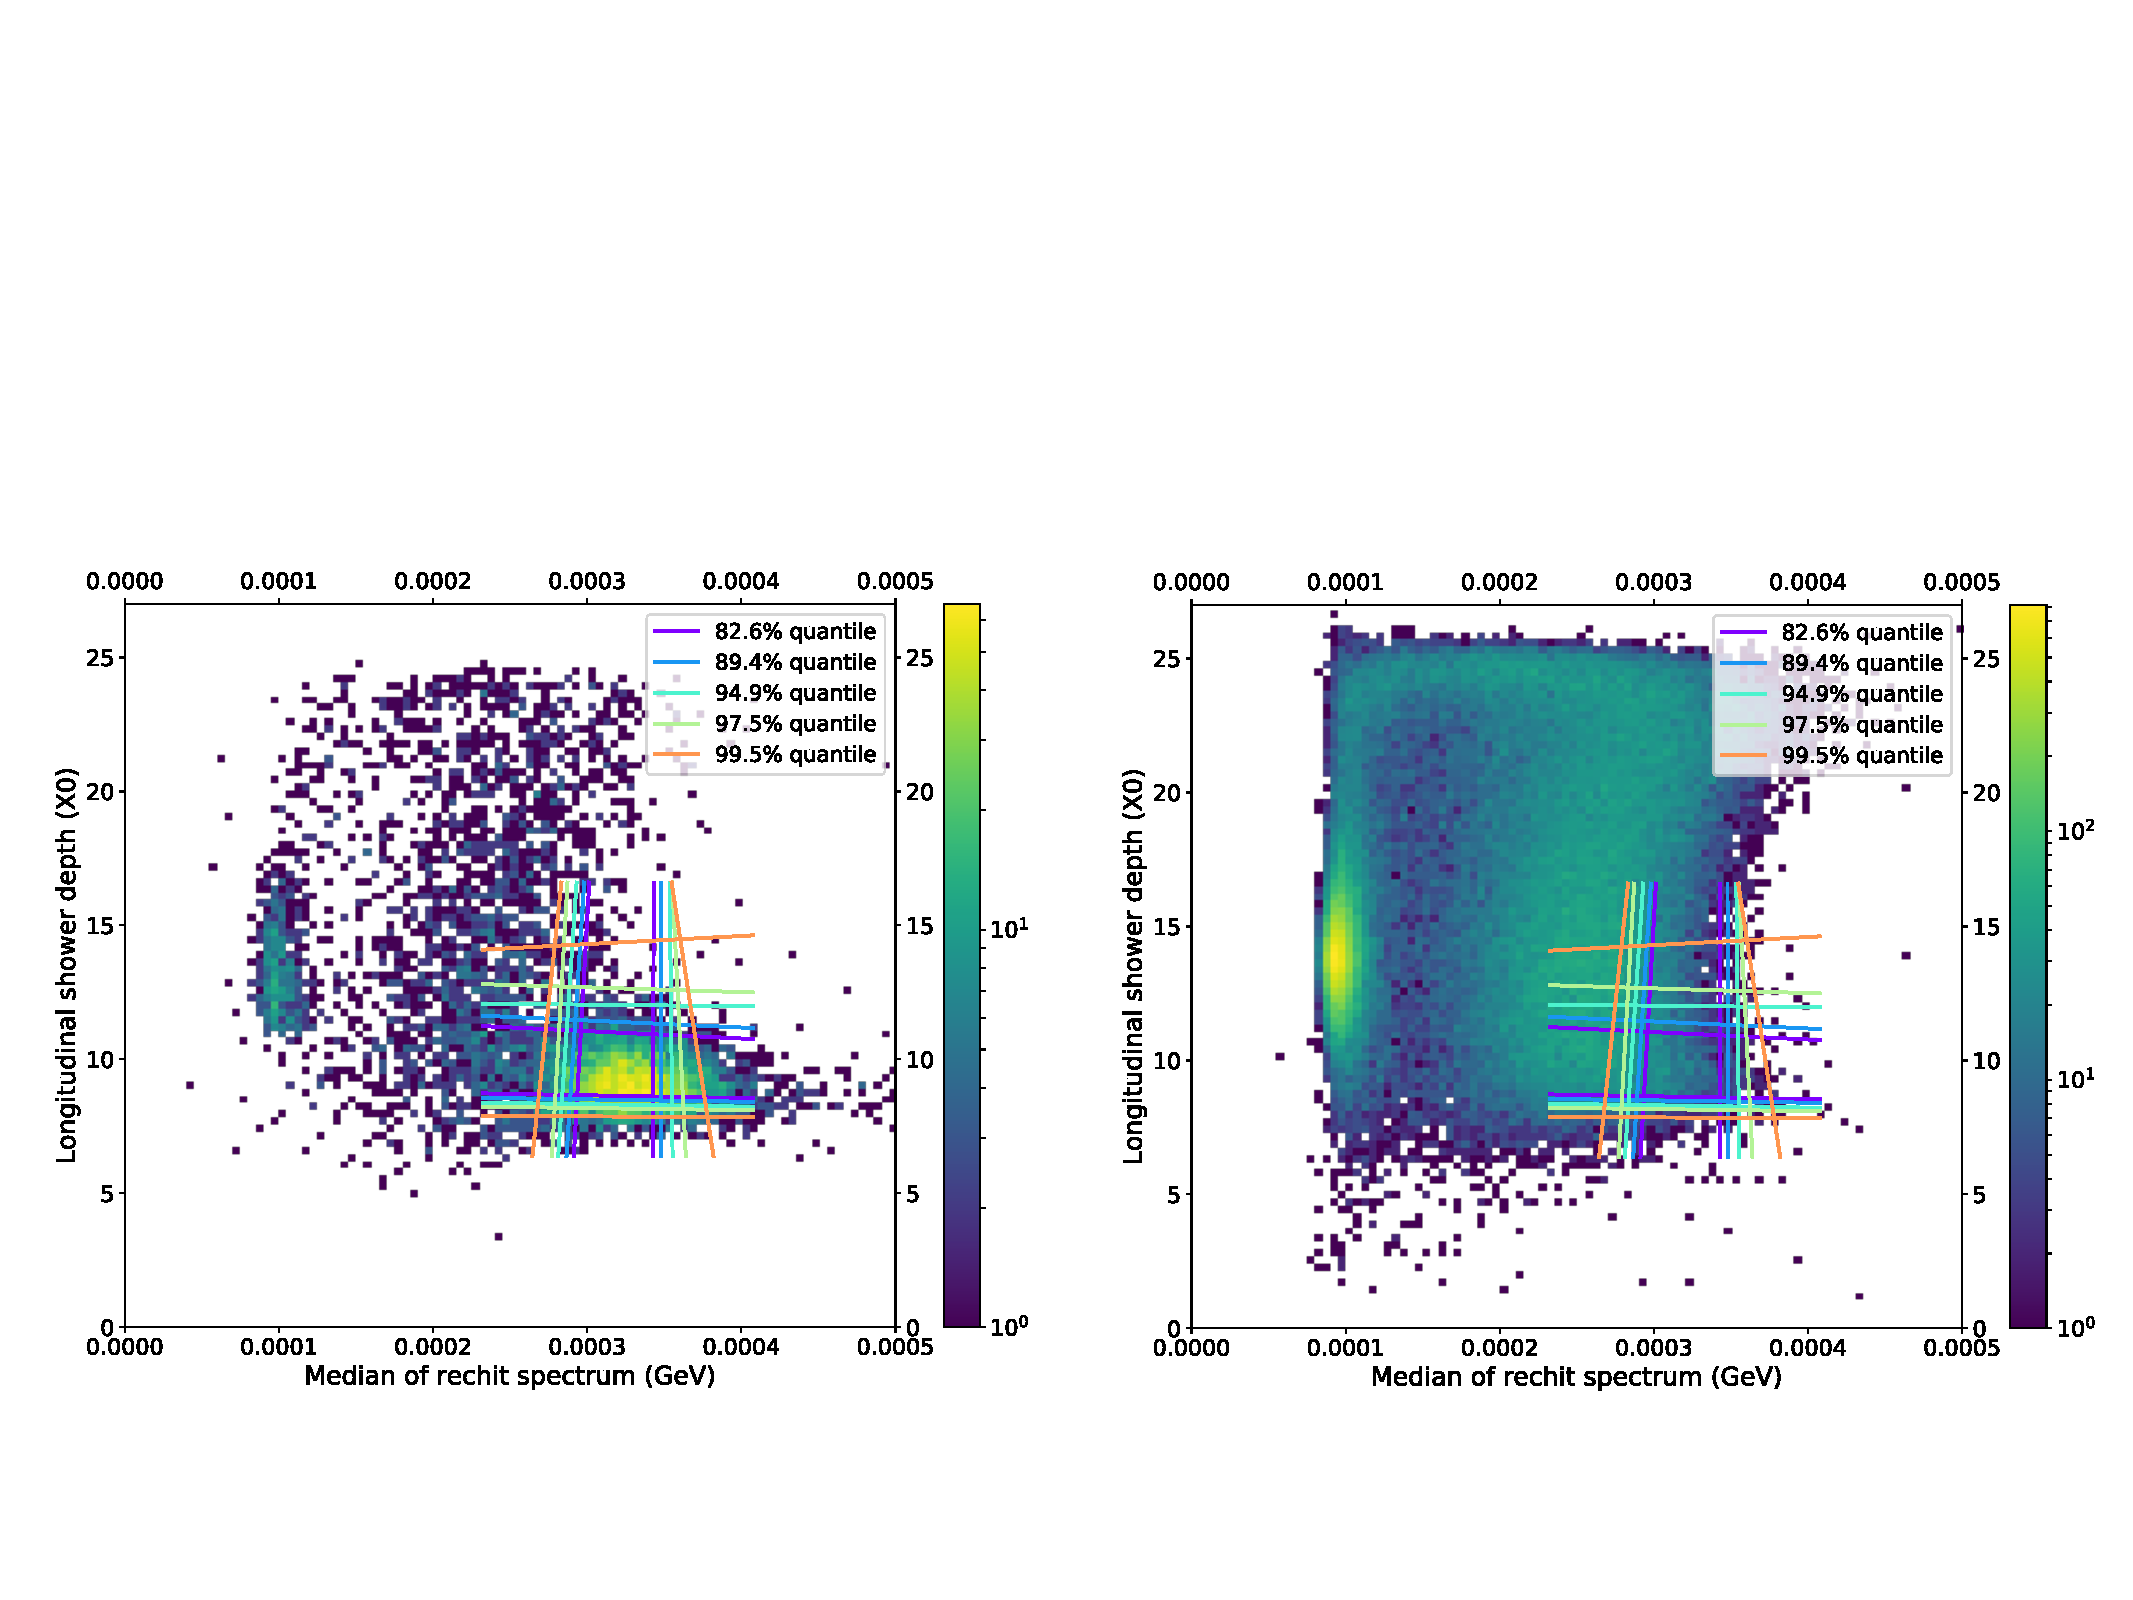
\includegraphics[width=1.0\textwidth]{Fig/fig_HGCAL/Window-Data-pion}~
    \caption{The "2-dimension window" cut applied on beamtest data and pion simulation samples.}
    \label{fig:2DHist-Window-Data-pion}
    \end{center}
\end{figure}

\begin{figure}[!ht]
    \begin{center}  
    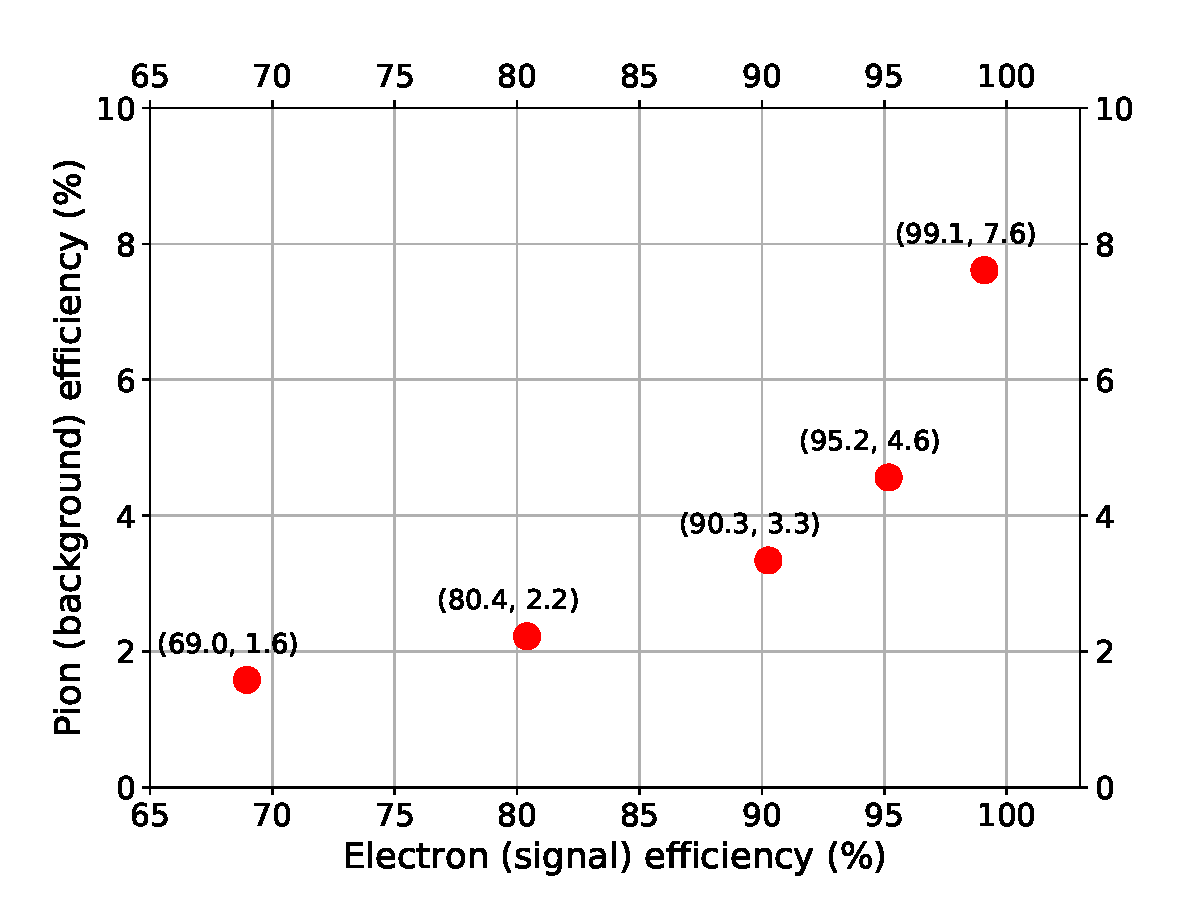
\includegraphics[width=0.5\textwidth]{Fig/fig_HGCAL/Working-Point-100GeV}~
    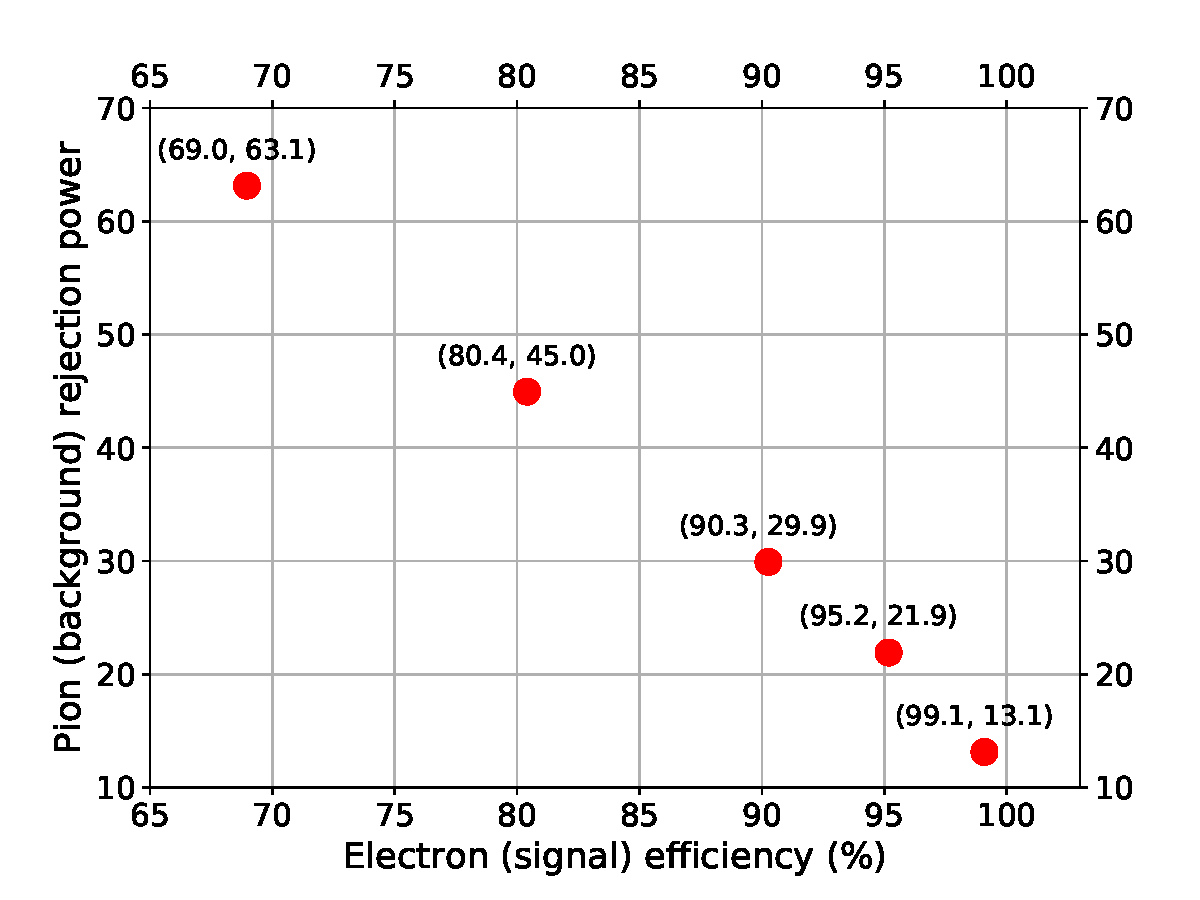
\includegraphics[width=0.5\textwidth]{Fig/fig_HGCAL/Working-Point-rejectionpower-100GeV}\\
    \caption{The electron (signal) efficiency as a function of the pion (background) efficiency (left) and The electron (signal) efficiencies as a function of background rejection power, defined as the reciprocal of background efficiency (right).}
    \label{fig:Window-WP}
    \end{center}
\end{figure}

The constructed window cut do not result in bias in the reconstructed energy, which can be seen in Fig.~\ref{fig:Etotal-WP-100GeV}, showing the distributions of total energy deposits in all layers with different working points, where all the distributions are normalized to unity. In the electron simulation sample, the tightest cut gives a 0.11\% of difference in the median of the distribution with respect to that without window cut, while in beamtest data the difference is 3.0\%.

\begin{figure}[!ht]
    \begin{center}  
    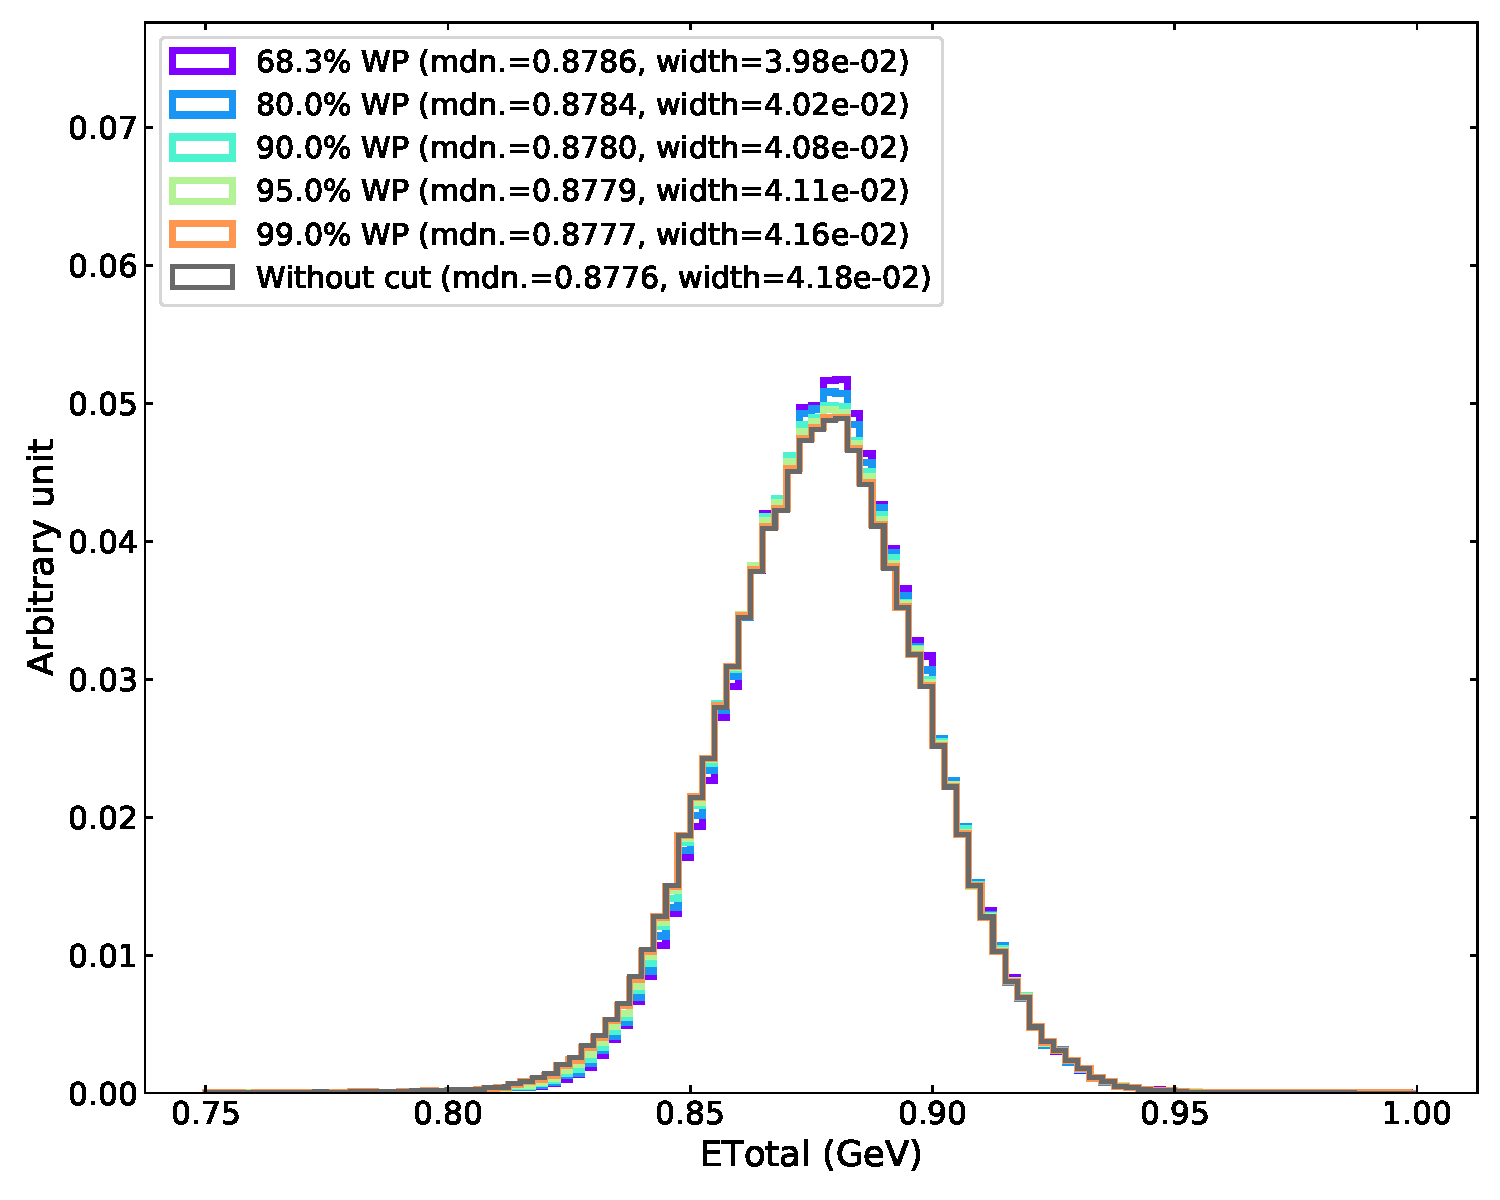
\includegraphics[width=0.5\textwidth]{Fig/fig_HGCAL/Etotal-WP-100GeV}~
    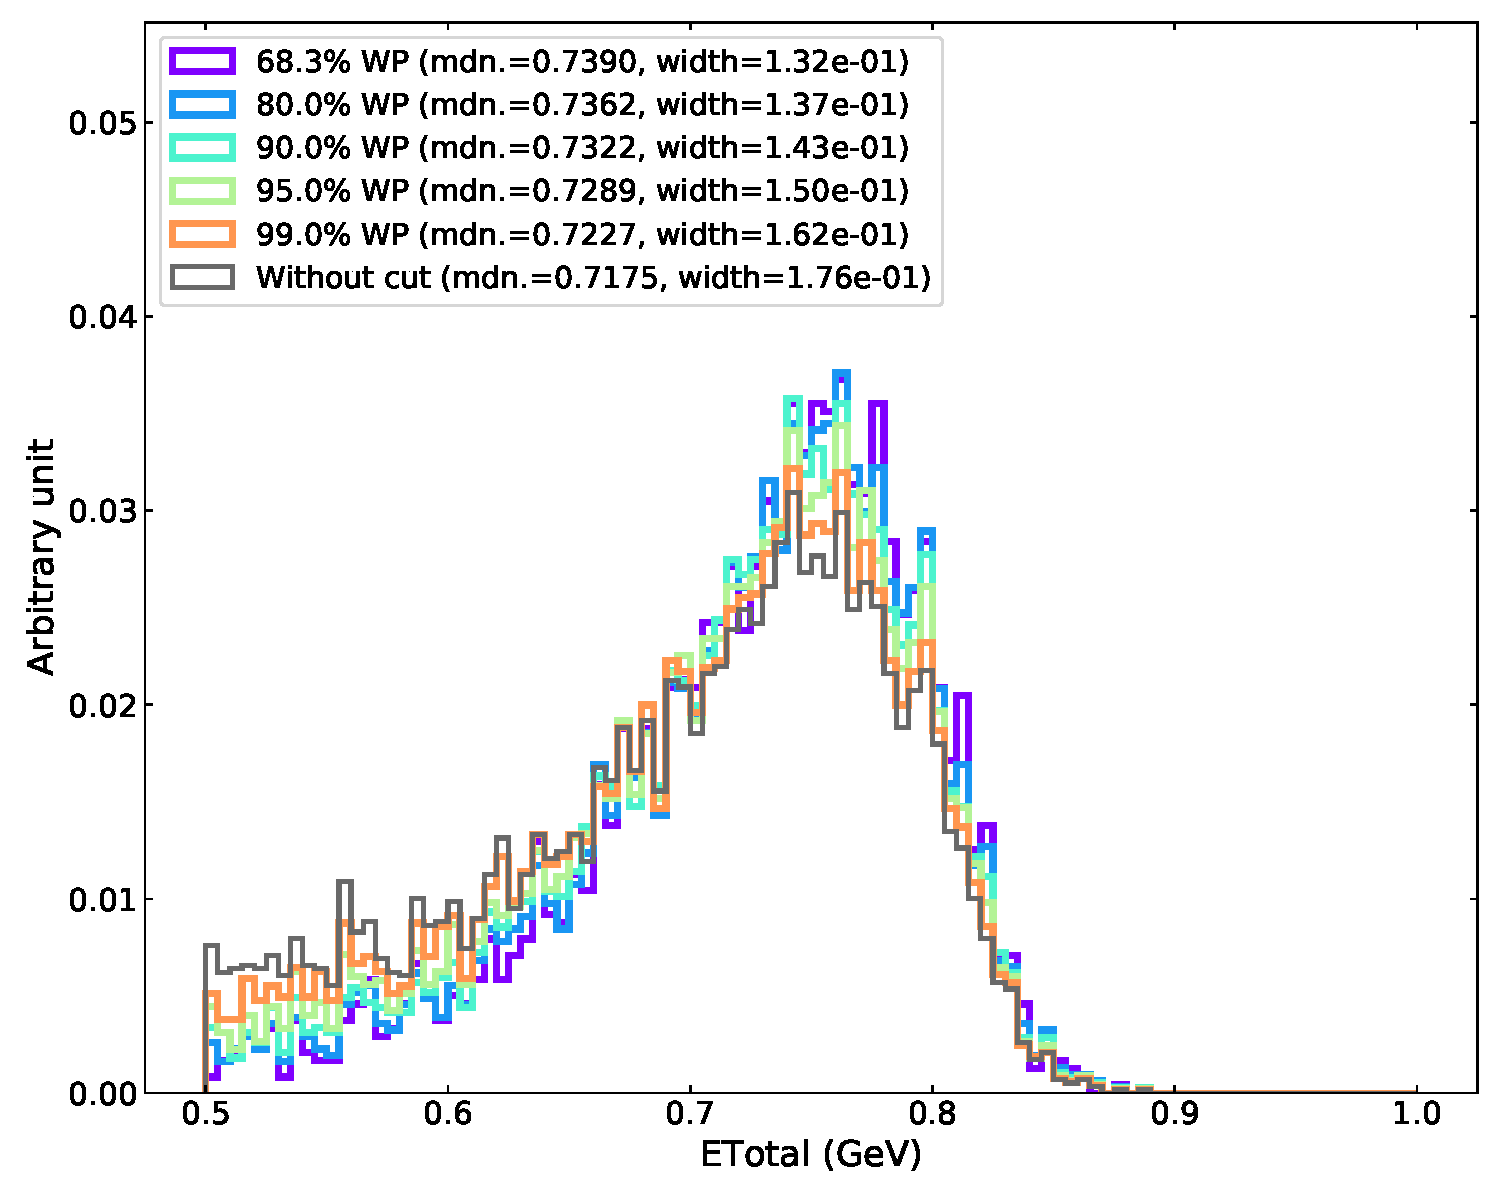
\includegraphics[width=0.5\textwidth]{Fig/fig_HGCAL/Etotal-WP-Junev11data-100GeV}\\
    \caption{The distributions of total energy deposits from simulation (left) and beamtest data (right) in all layers with different working points, where all the distributions are normalized to unity.}
    \label{fig:Etotal-WP-100GeV}
    \end{center}
\end{figure}

Fig.~\ref{fig:DataMC-comparison} shows the comparisons of EAll of layer 1, E7/E19 of layer 1, and sum of EAll/Etot over layer 1 to 10 between the beamtest data and simulation samples for both electron and pion events, the plots in left column are without applying the window cut and the plots on the right are with the window cuts of 68.3\% working point. The agreement of the distributions between beamtest data and simulations of electron events improves after applying the tightest window cut. There are still residual pion events mimicking electrons after applying the tightest window cut, meaning that those pion events cannot be distinguished by this window cut. This can be seen from the event displays, Fig.~\ref{fig:EvDisplay-pion-window}, of the pion simulation events that contained in the window cut. A more powerful identification is needed if one wants purer electron samples from beamtest data. The machine learning technique is proposed and tested, and will be discussed in the next subsection.

\begin{figure}[p]
    \begin{center}  
    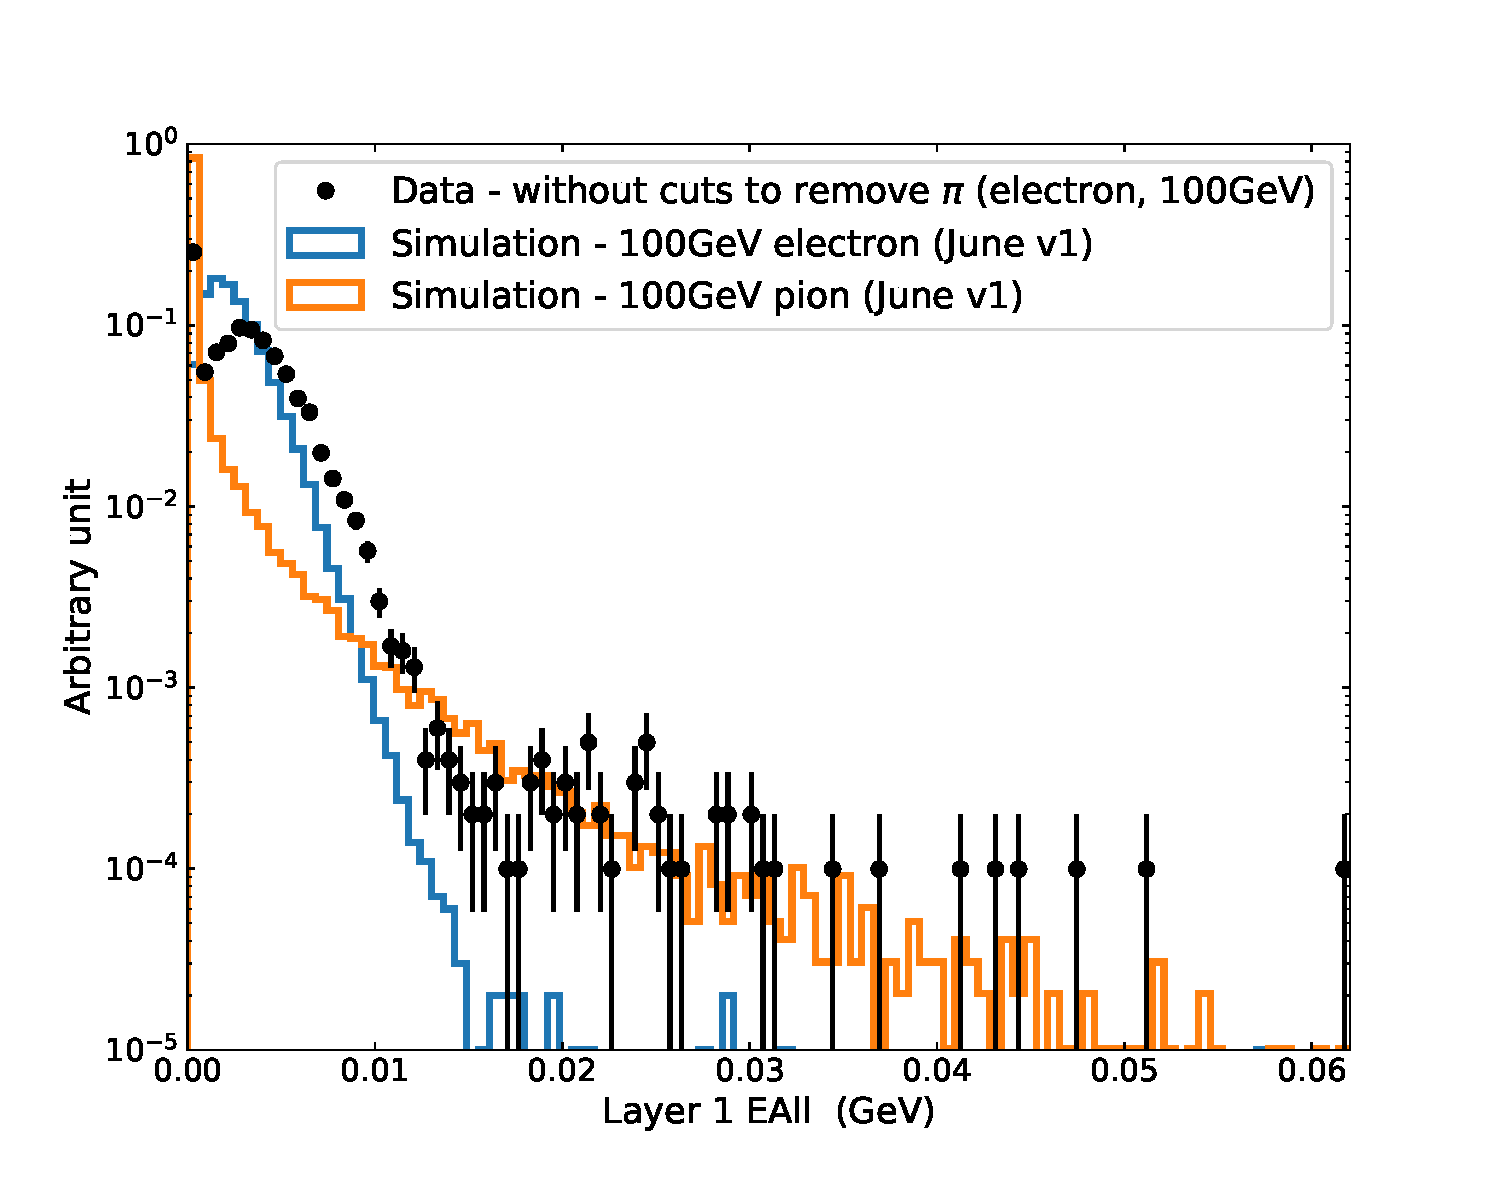
\includegraphics[width=0.5\textwidth]{Fig/fig_HGCAL/L1-EAll-GeV-NoWindow}~
    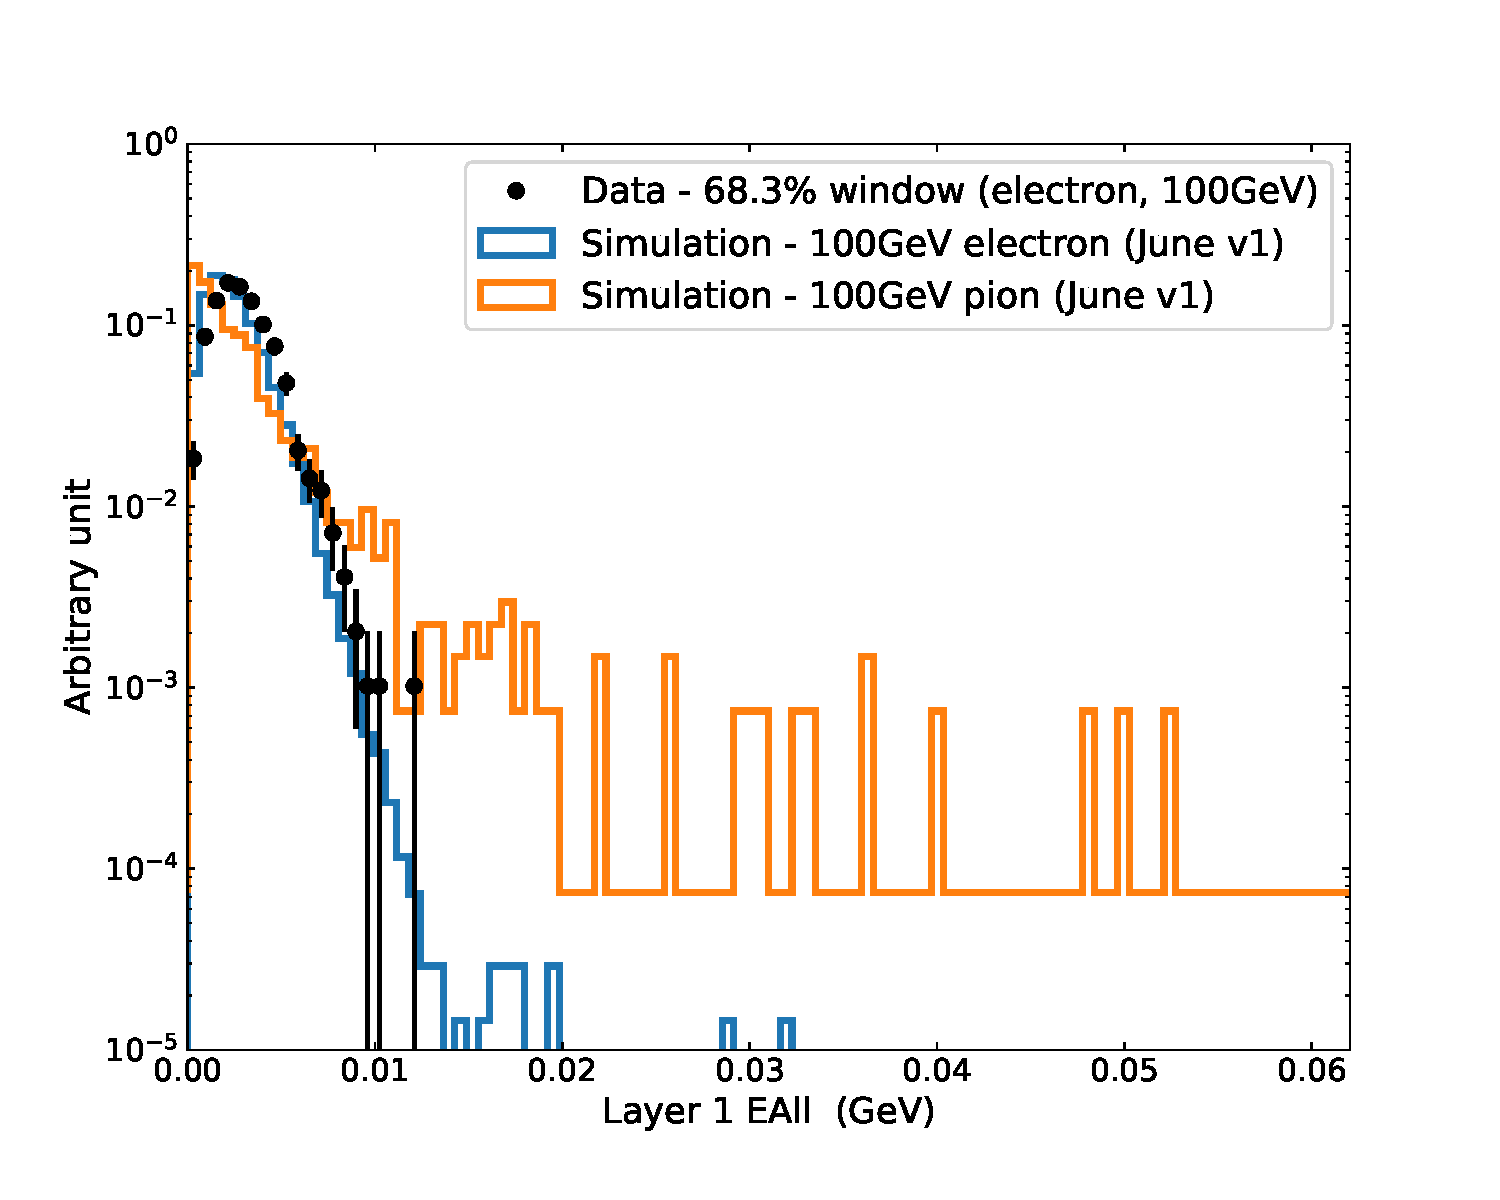
\includegraphics[width=0.5\textwidth]{Fig/fig_HGCAL/L1-EAll-GeV-WP68}\\
    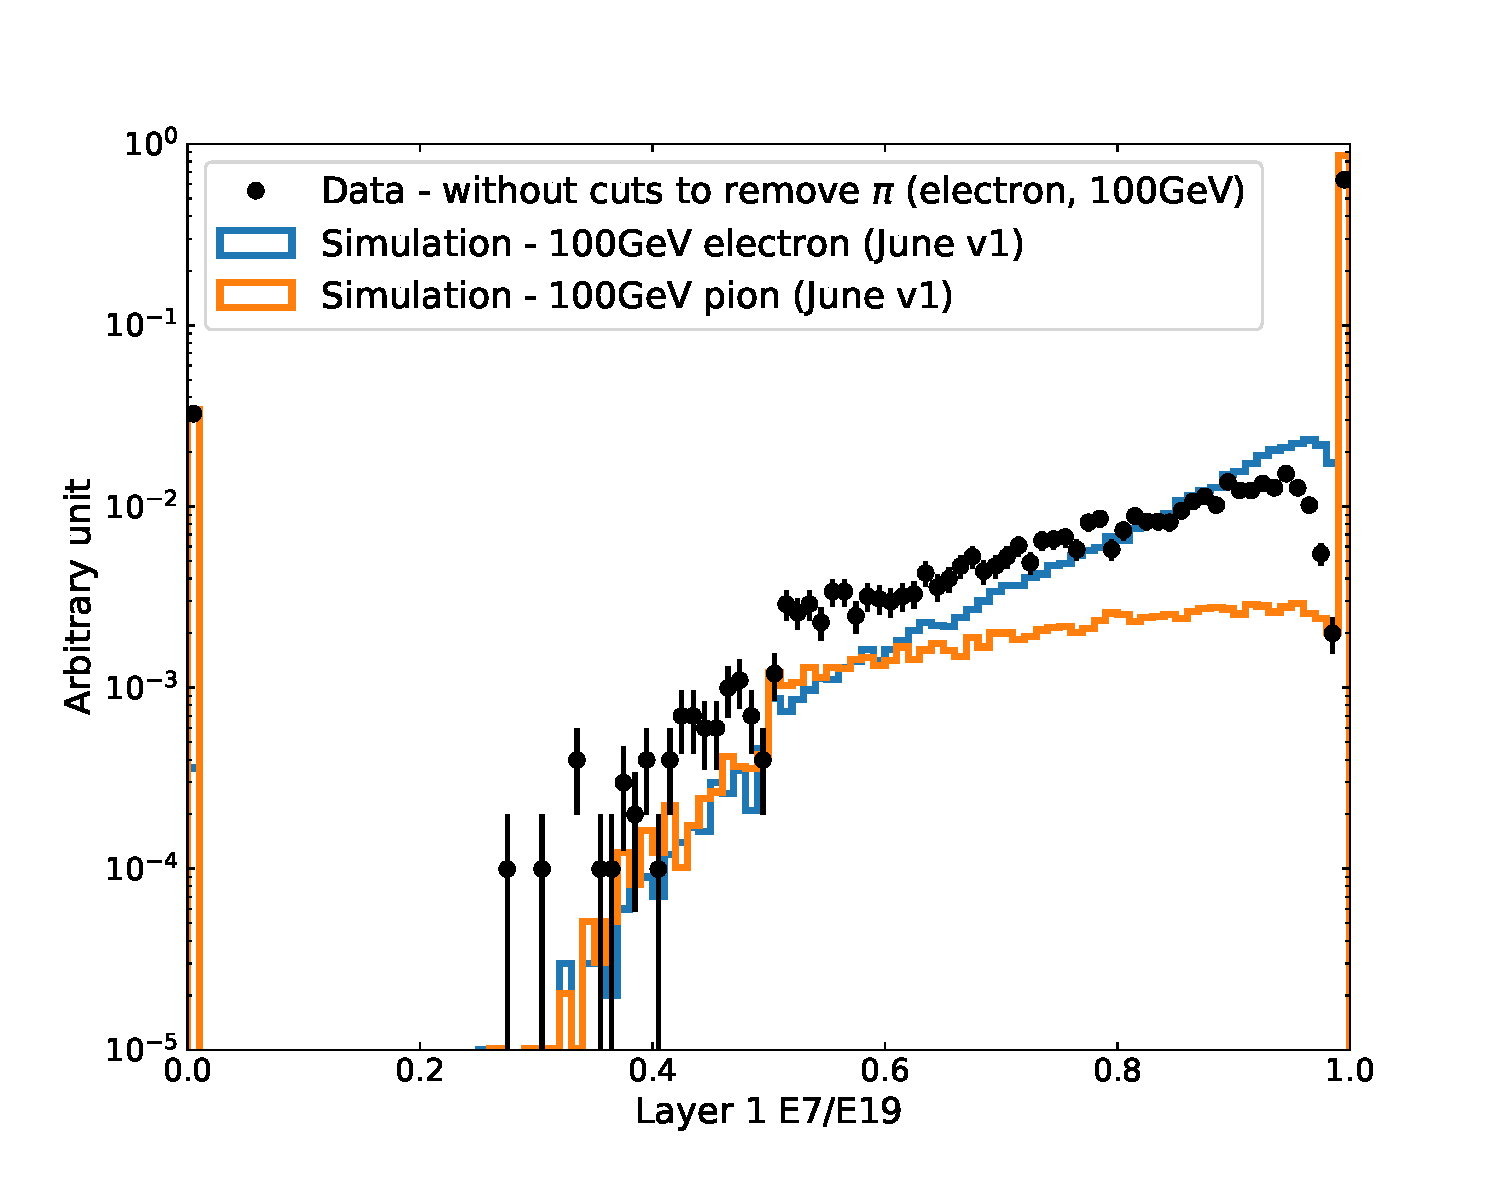
\includegraphics[width=0.5\textwidth]{Fig/fig_HGCAL/L1-sum7-over-sum19-NoWindow}~
    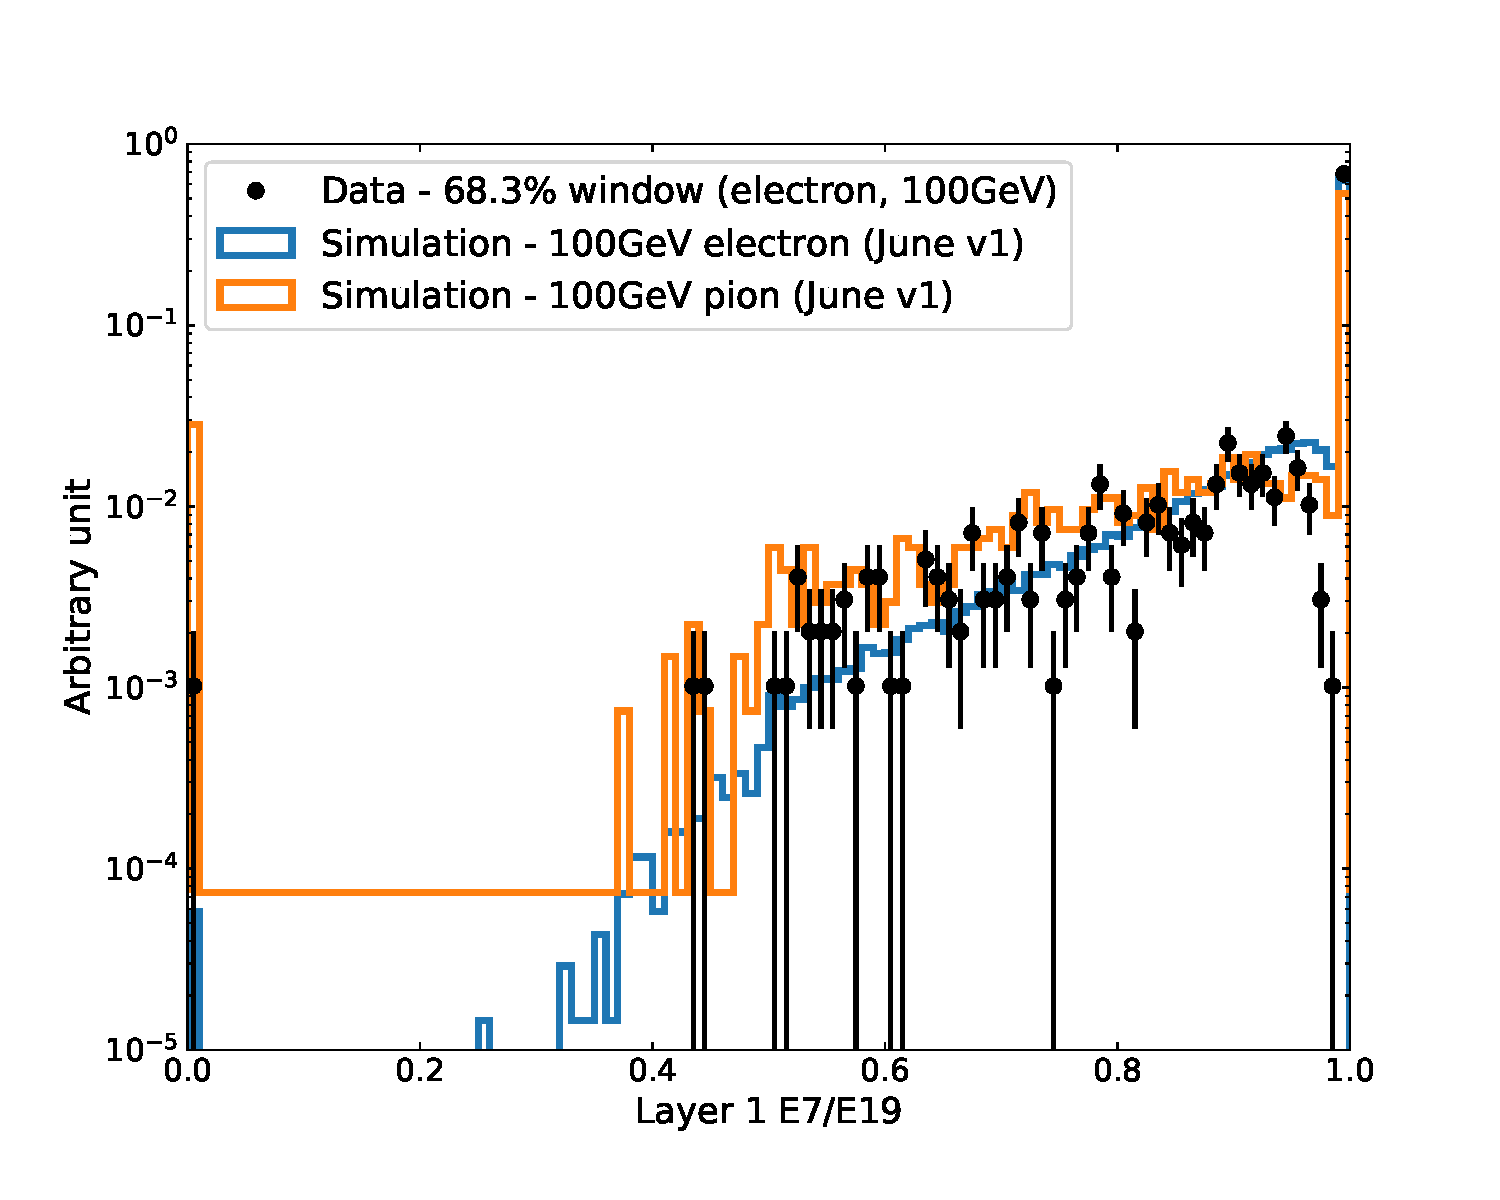
\includegraphics[width=0.5\textwidth]{Fig/fig_HGCAL/L1-sum7-over-sum19-WP68}\\
    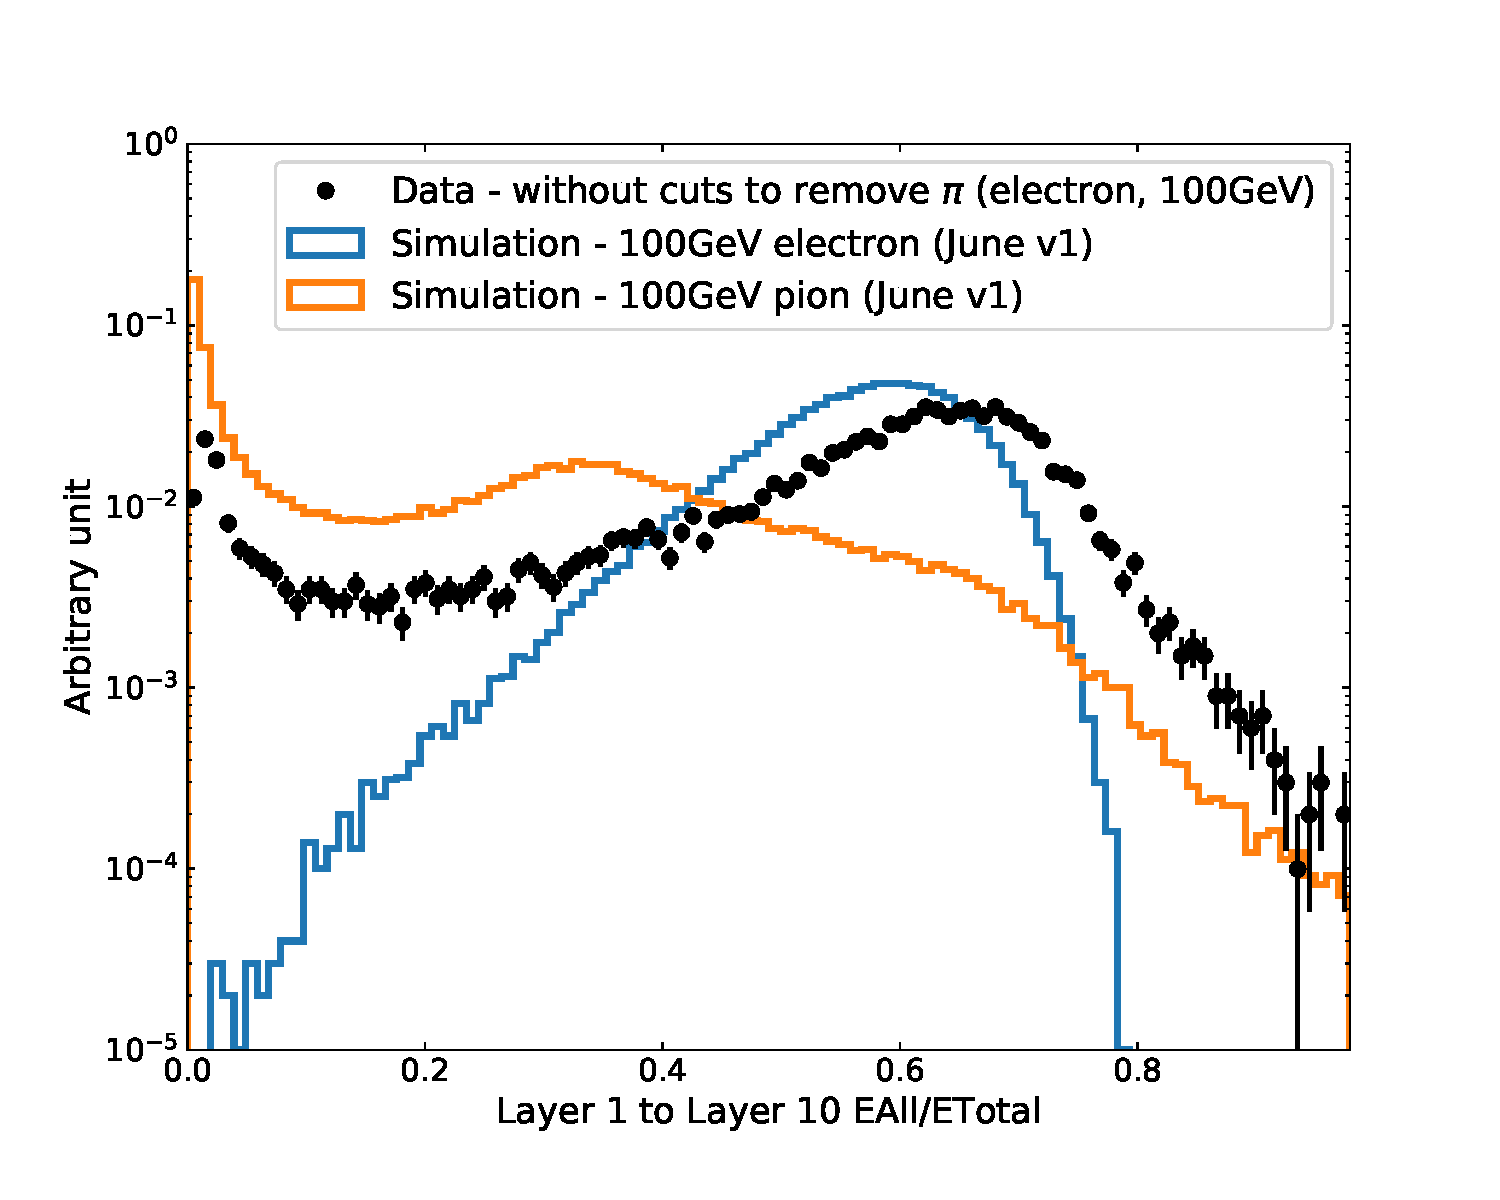
\includegraphics[width=0.5\textwidth]{Fig/fig_HGCAL/L1toL10-EAll-over-ETotal-NoWindow}~
    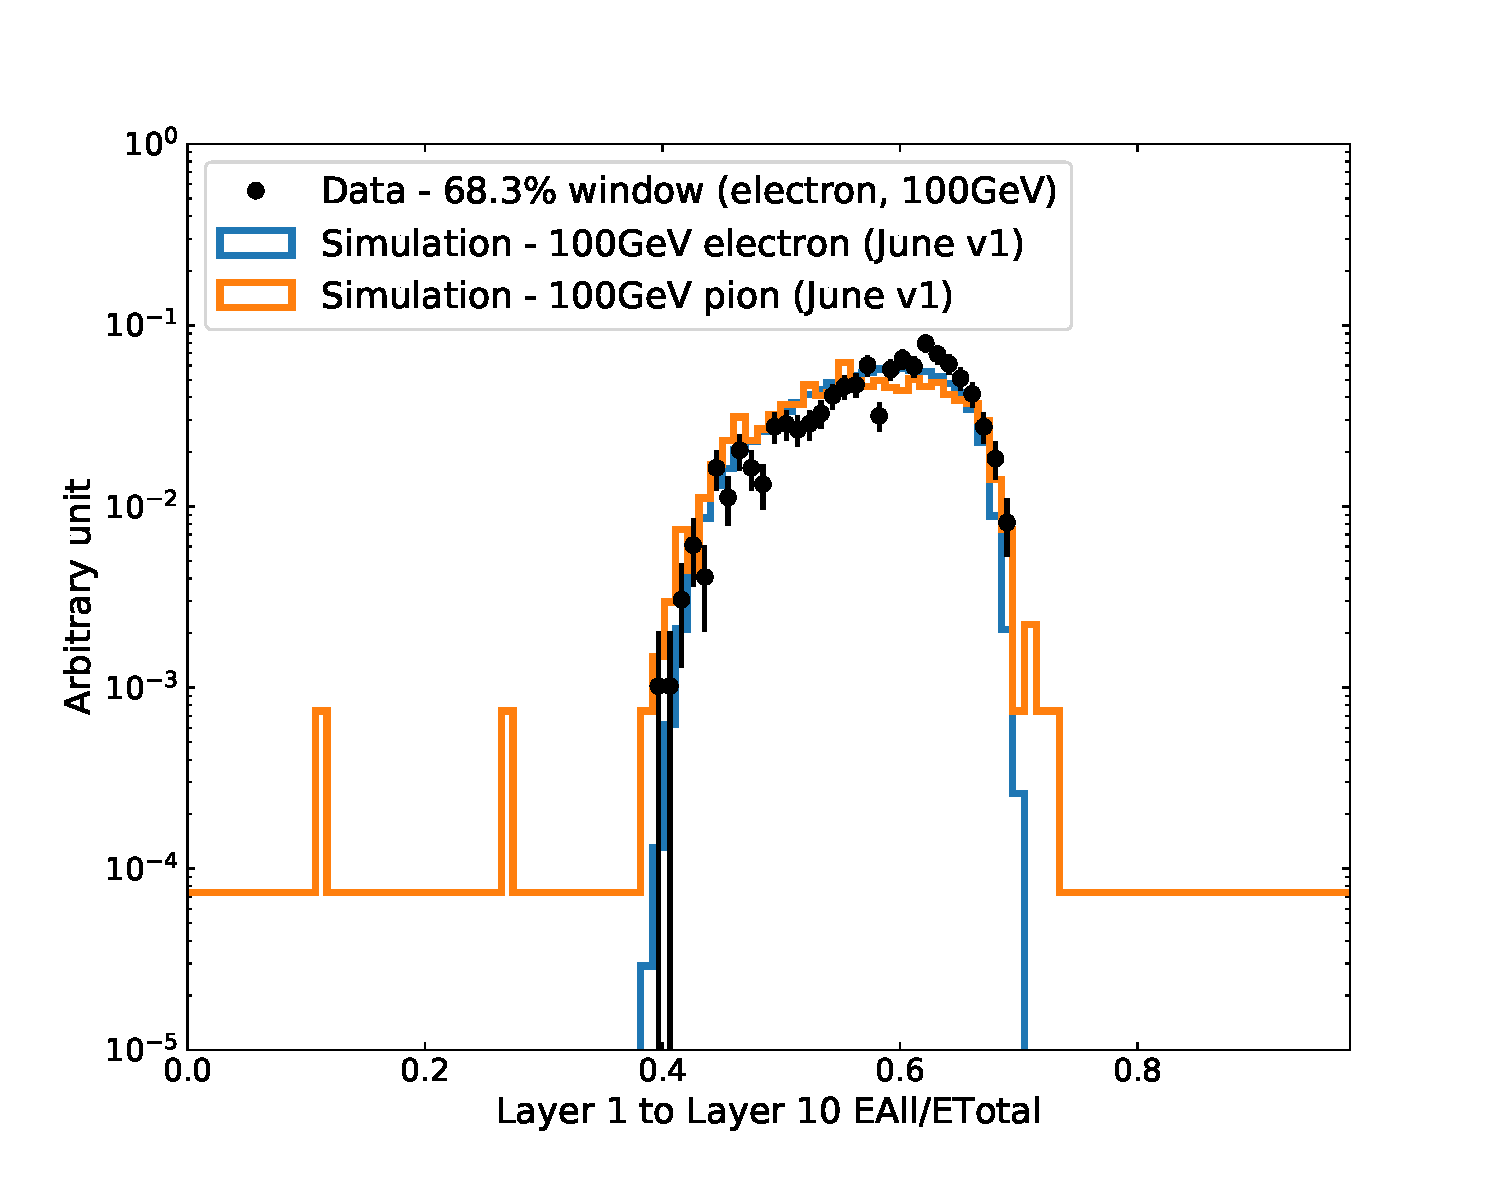
\includegraphics[width=0.5\textwidth]{Fig/fig_HGCAL/L1toL10-EAll-over-ETotal-WP68}\\
    \caption{The comparison between the beamtest data and simulation samples for both electron and pion events, the plots in left row are without applying the window cut and the plots on the right are with the window cuts of 68.3\% working point.}
    \label{fig:DataMC-comparison}
    \end{center}
\end{figure}

\begin{figure}[p]
    \begin{center}  
    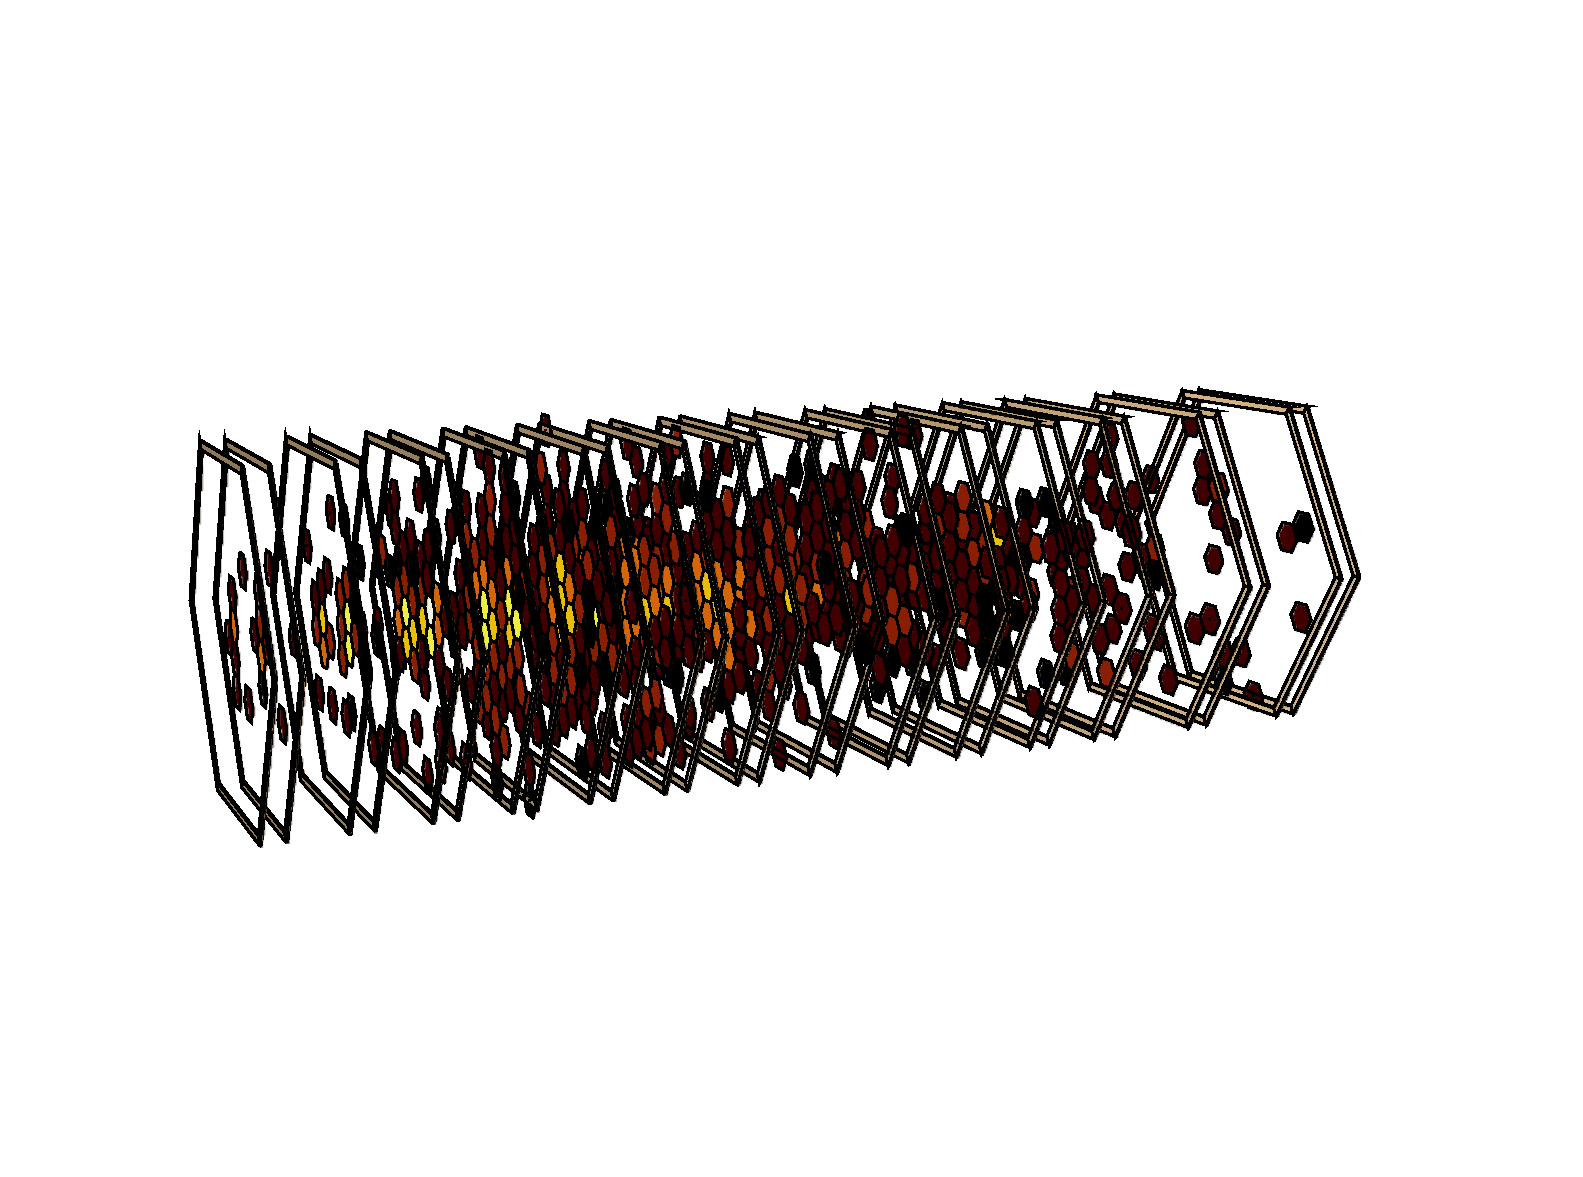
\includegraphics[width=1.0\textwidth]{Fig/fig_HGCAL/EvDisplay3D-pion-100GeV-Junev1sim-event102}\\
    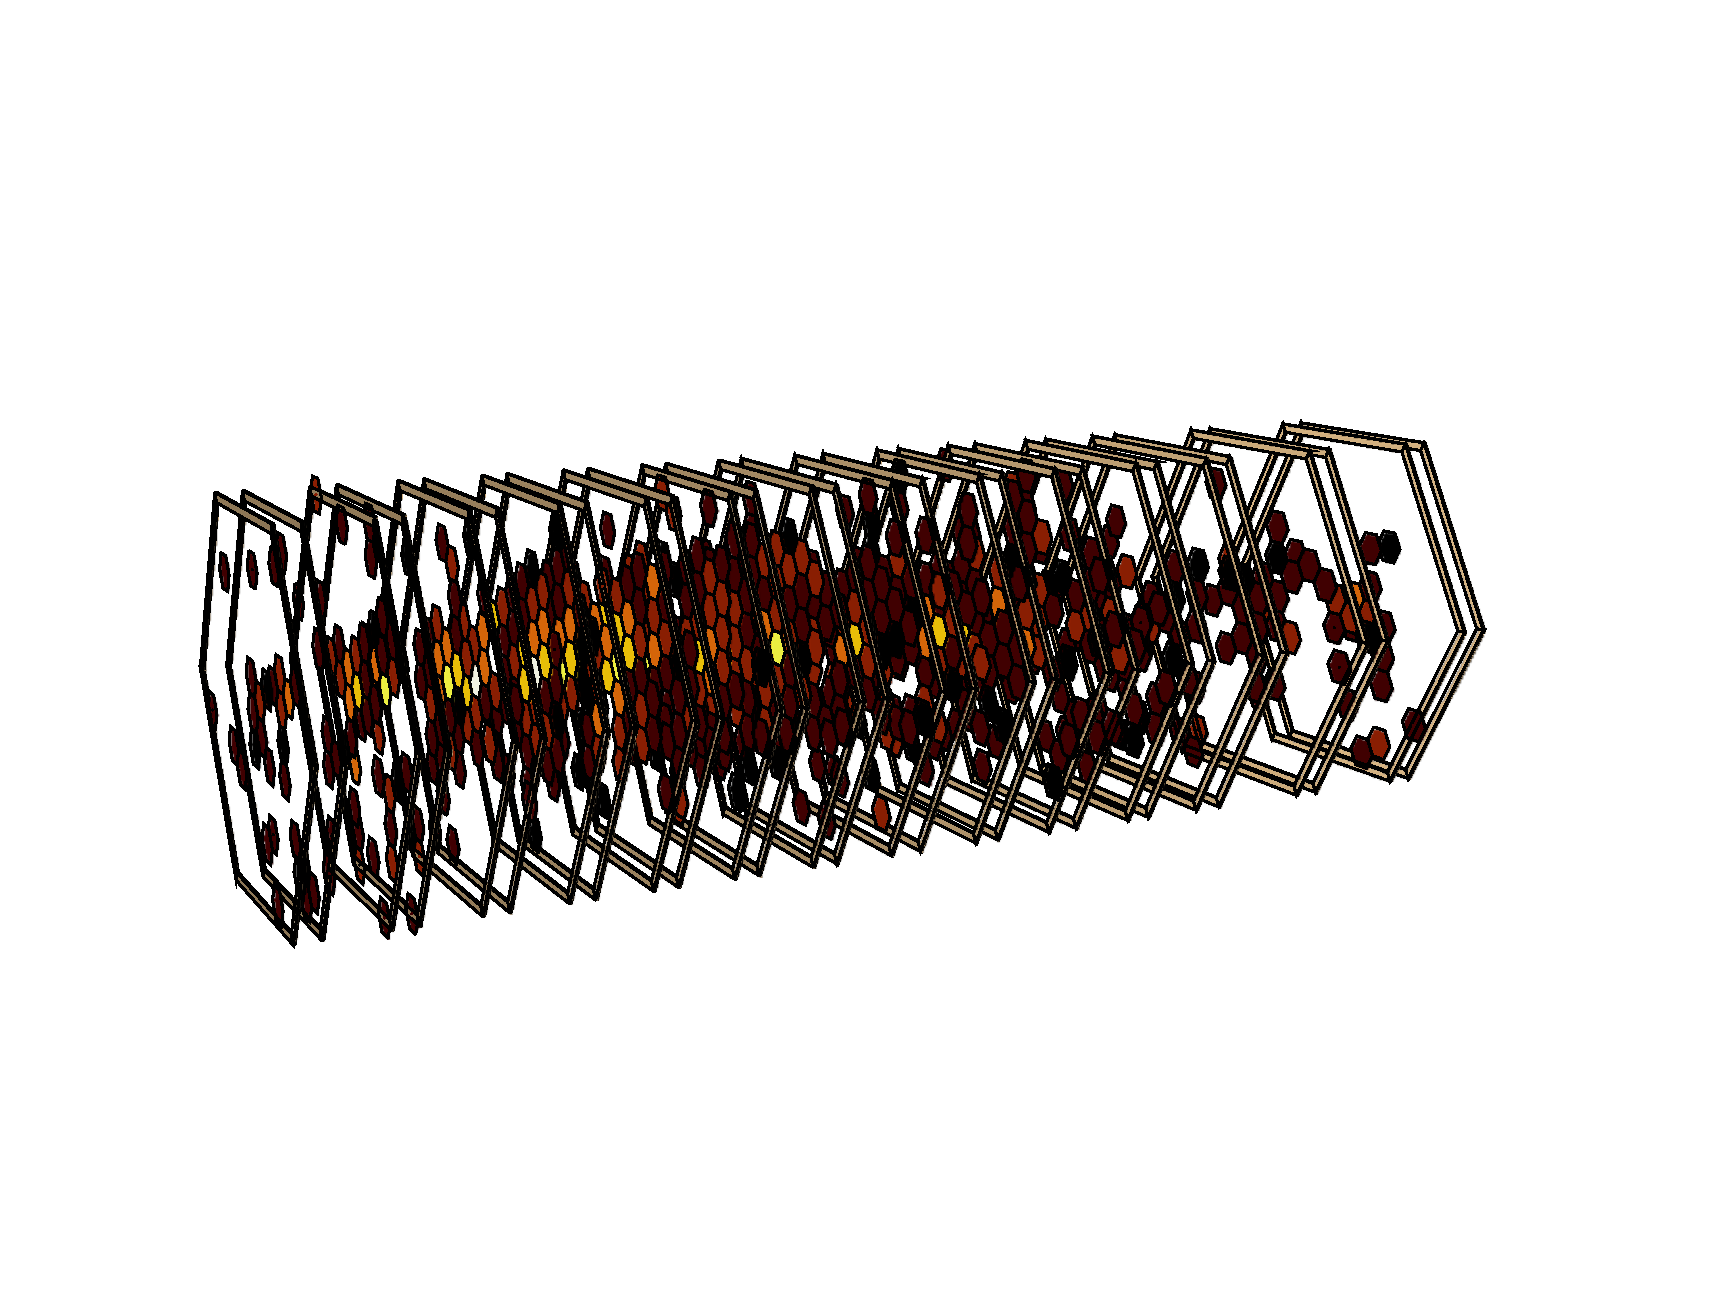
\includegraphics[width=1.0\textwidth]{Fig/fig_HGCAL/EvDisplay3D-pion-100GeV-Junev1sim-event388}\\
    \caption{Examples of event display of the pion events that contained in the window cut.}
    \label{fig:EvDisplay-pion-window}
    \end{center}
\end{figure}

\section{Machine learning technique for Electron and pion separation}
\label{sec:ElectronID-BDT}
In the first step, I tried using mdn of RecHit and depthX0 as training features for the classifier. This should give the baseline performance for the multivariate identification. Four commonly used classifiers are tested 
\begin{itemize}  
\item Linear support vector machine (linear SVM)
\item XGBClassifier, based on gradient boosting algorithm
\item Adaptive boosting classifier (AdaBoostClassifier)
\item Random forest classifier (RandomForestClassifier)
\end{itemize}
The details of the classifiers and the corresponding algorithms will not be described in this report. 
The classifier outputs\footnotemark from tested classifiers are shown in Fig.~\ref{fig:Classifier-Output}, and the receiver operating characteristic (ROC) curves obtained from the classifier outputs are in Fig.~\ref{fig:ROCcurves}.
The hyper-parameters used in the classifiers are the default setting of XGBClassifier. Table.~\ref{tab:ROC-summary} summarizes the background (pion) efficiency with 99.0\% of signal (electron) efficiency from each tested classifier, which quantifies the performance on electron and pion separation. Among the four classifiers, XGBClassifier gives the best performance on discriminating the electron and pion events, resulting an 2.2\% of improvement with respect to the window cut. 
Therefore, XGBClassifier will be used as the classifier in the following study.
\footnotetext{The value of classifier output is defined as the probability of each event being predicted as electron.}
\clearpage


\begin{figure}[!ht]
    \begin{center}  
    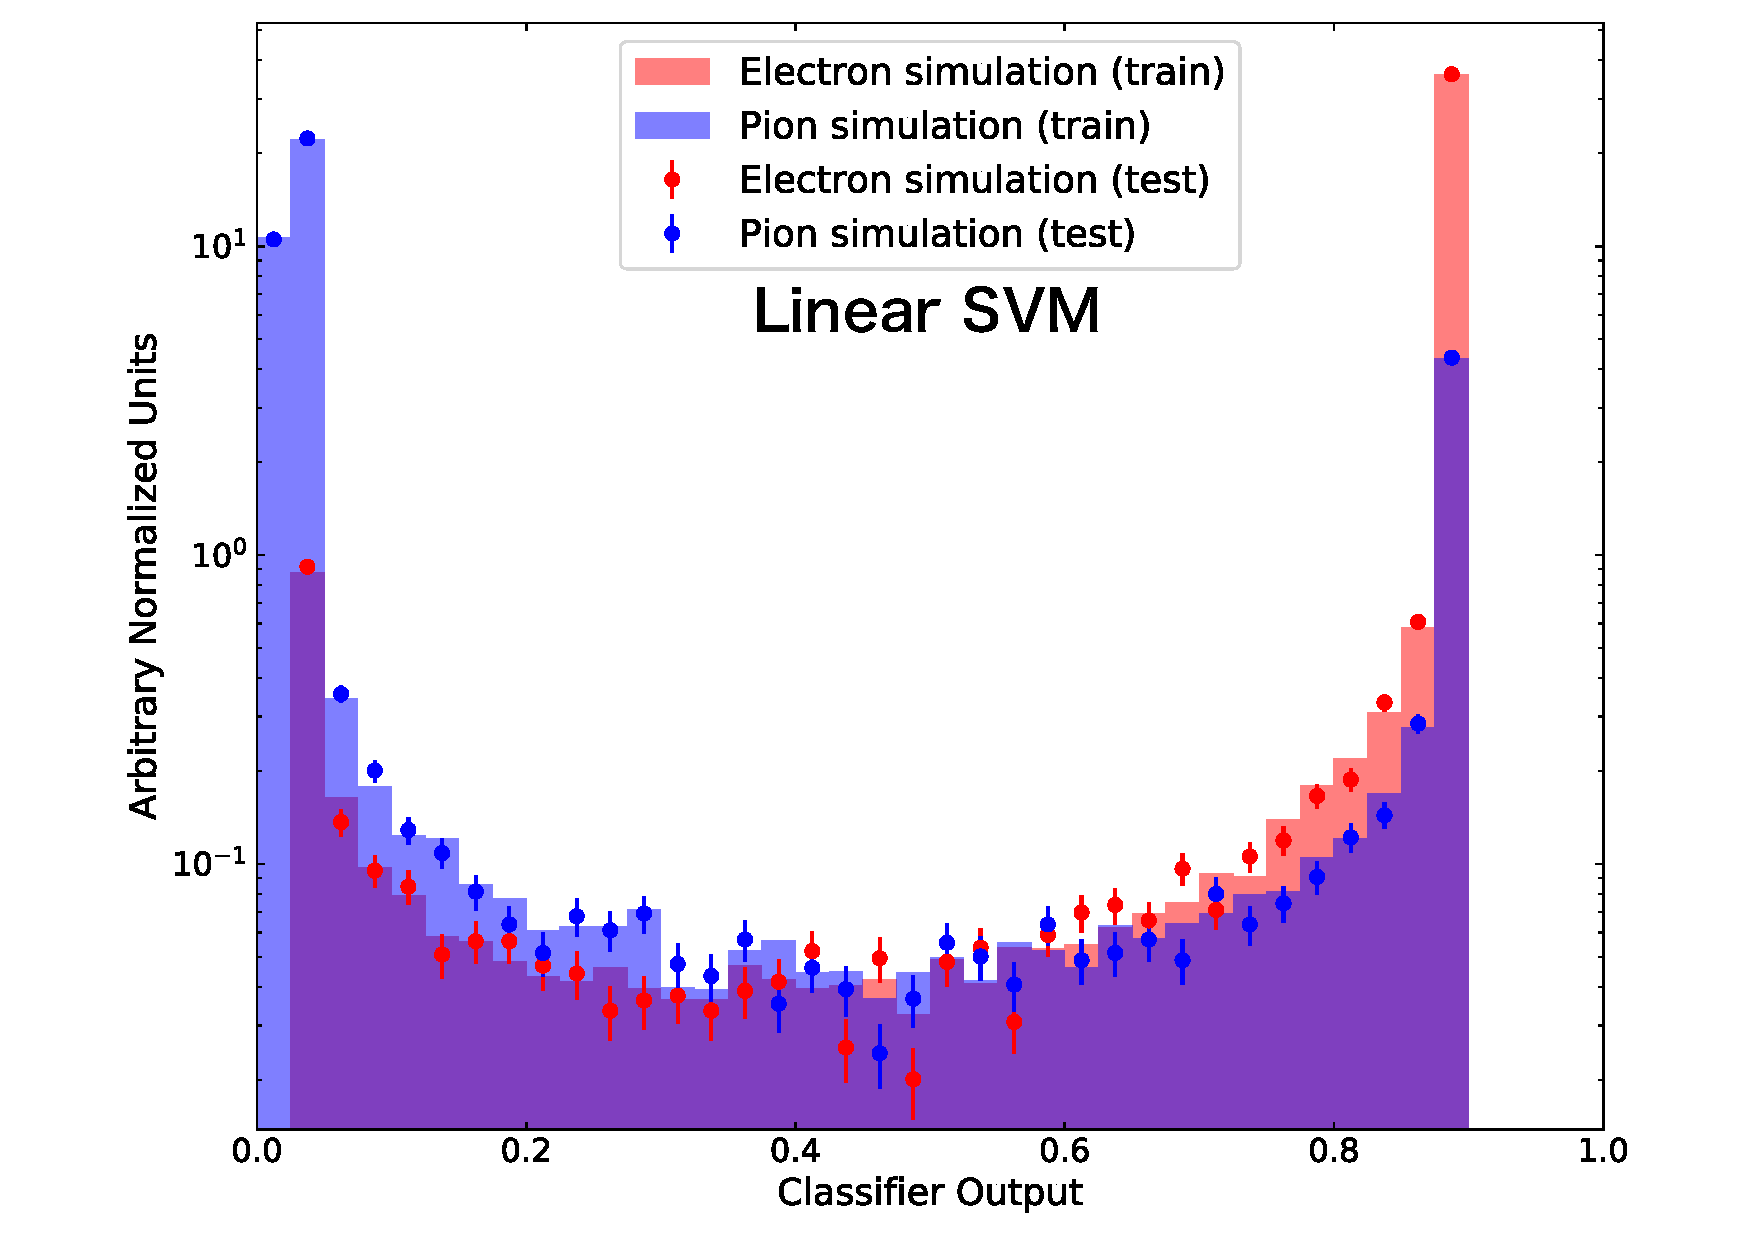
\includegraphics[width=0.5\textwidth]{Fig/fig_HGCAL/Classifier-output-2vars-SVM}~
    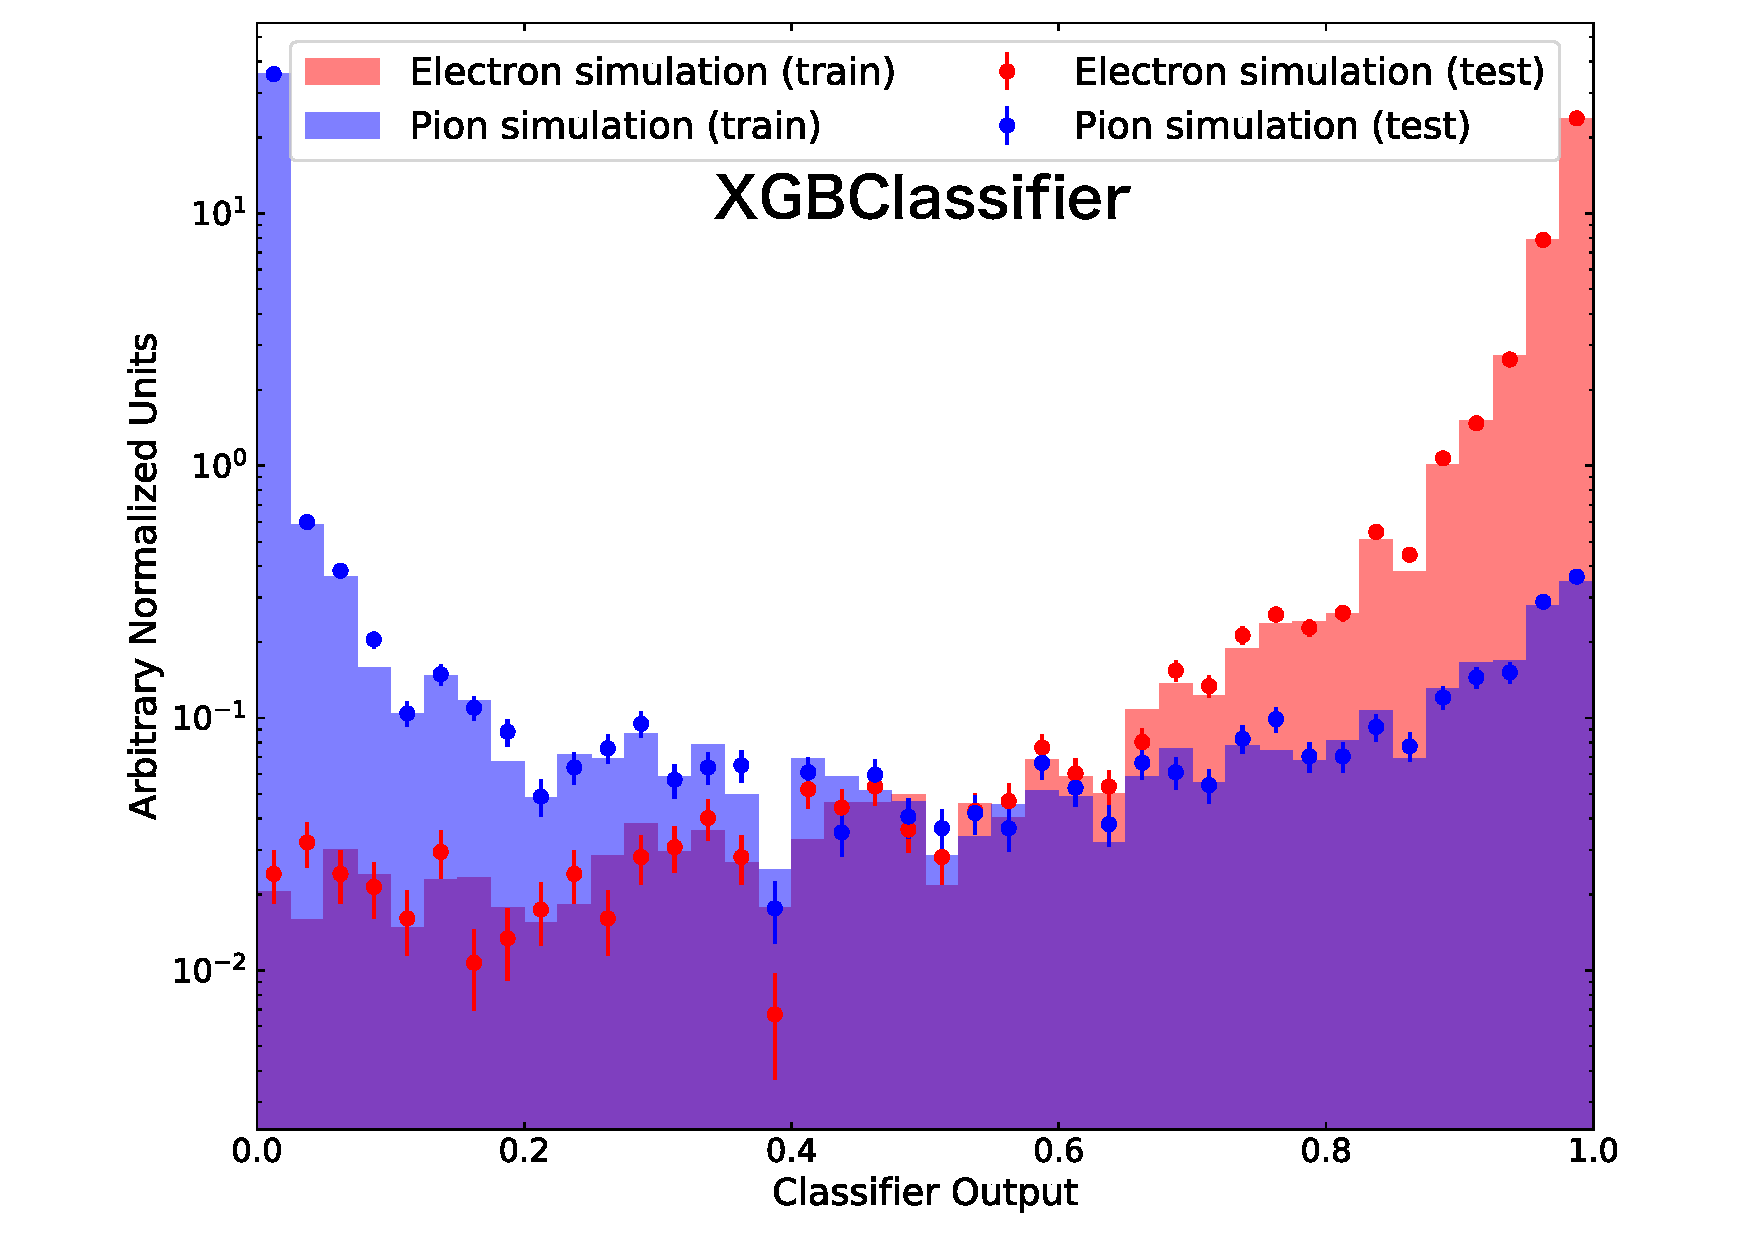
\includegraphics[width=0.5\textwidth]{Fig/fig_HGCAL/Classifier-output-2vars-XGBClassifier}\\
    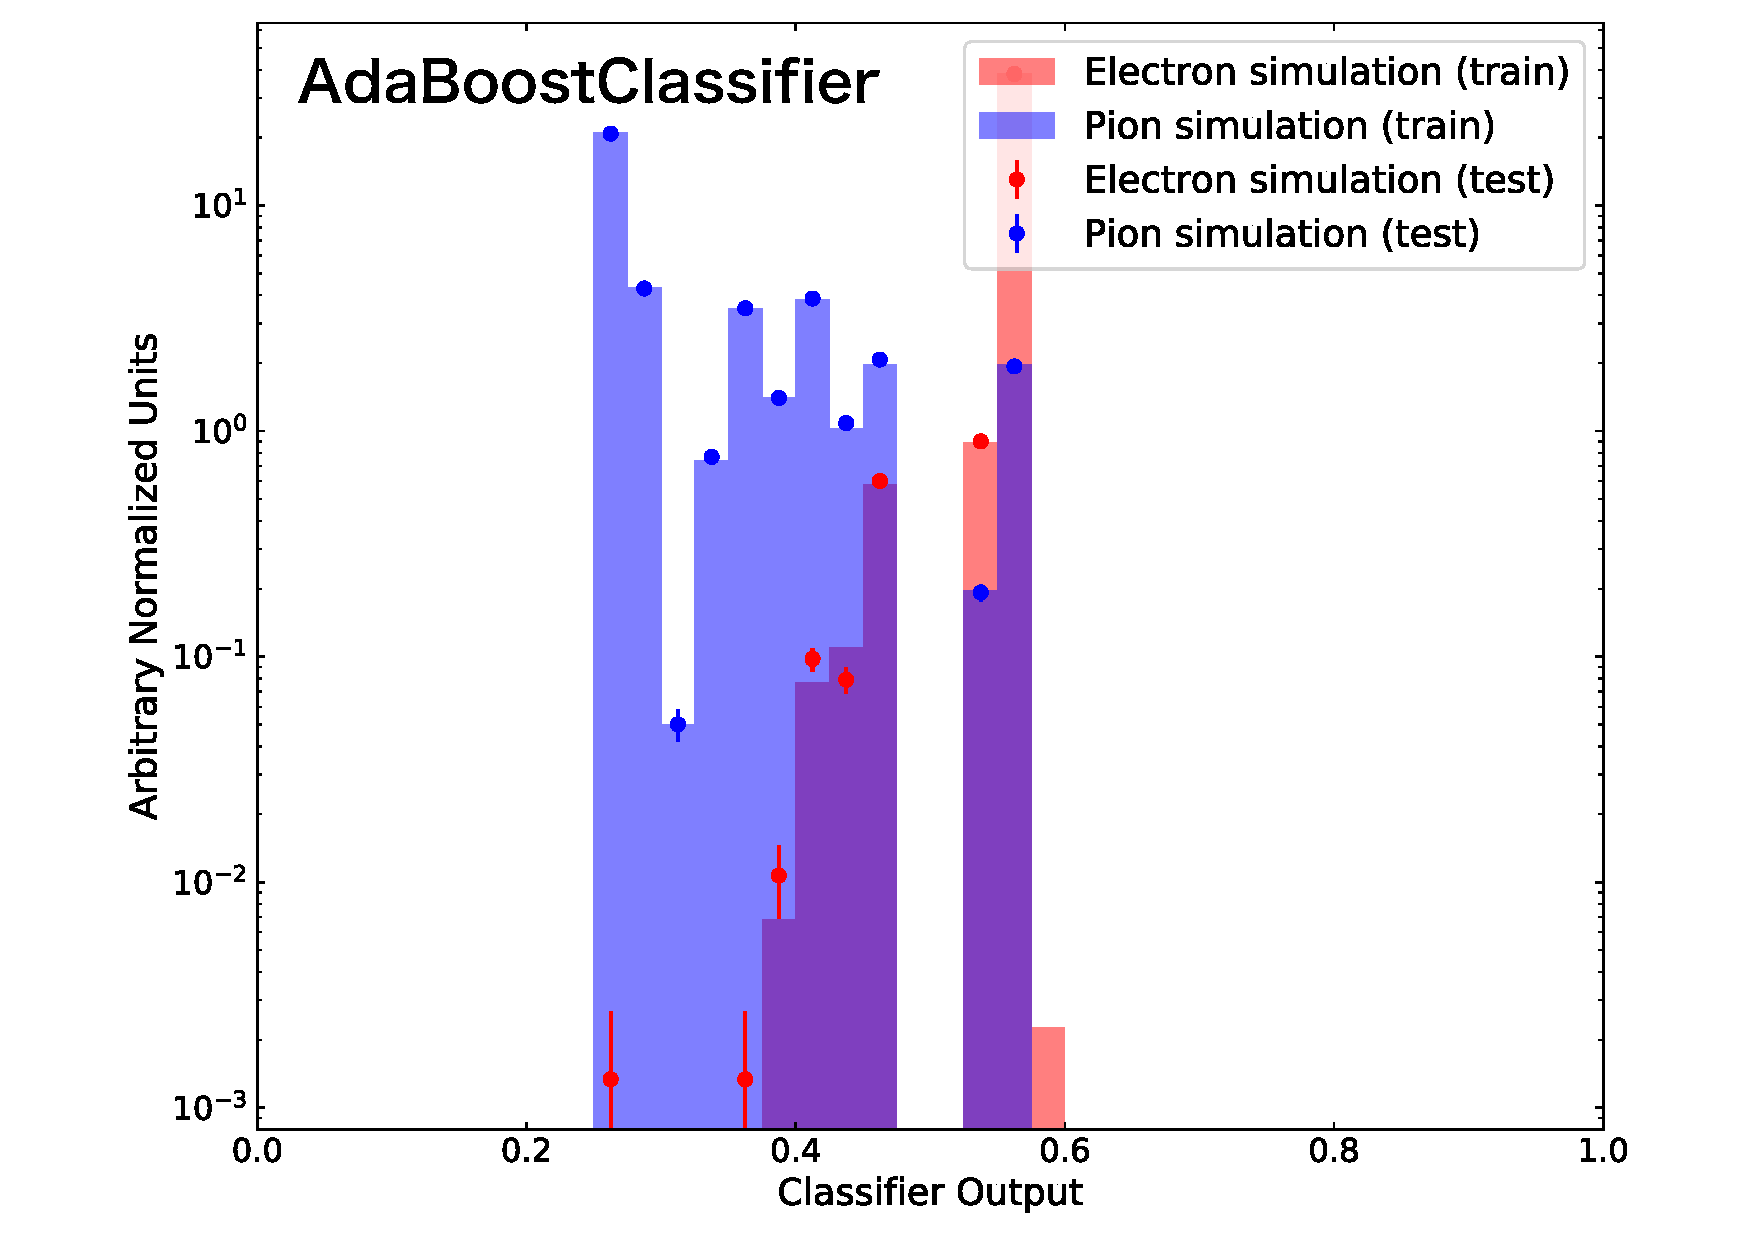
\includegraphics[width=0.5\textwidth]{Fig/fig_HGCAL/Classifier-output-2vars-AdaBoost}~
    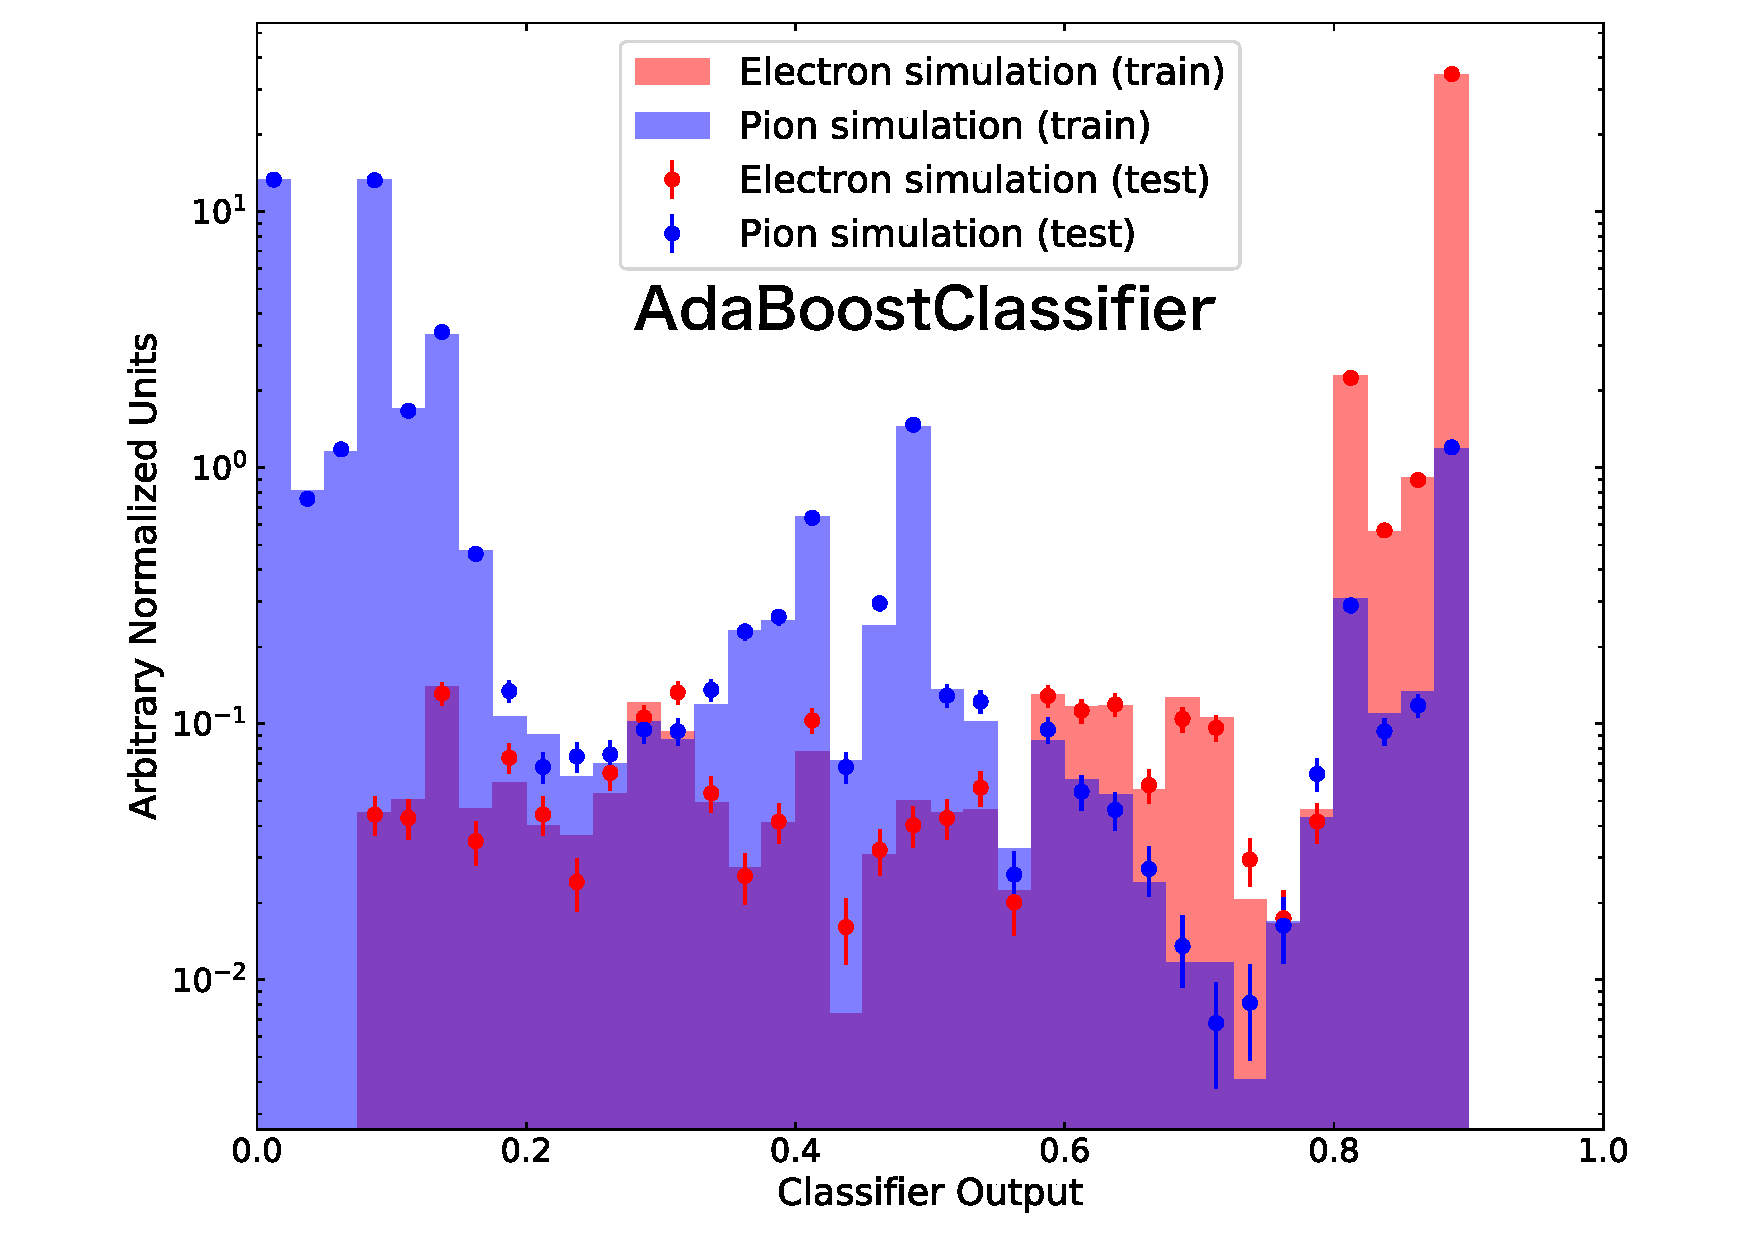
\includegraphics[width=0.5\textwidth]{Fig/fig_HGCAL/Classifier-output-2vars-RandomForest}\\1
    \caption{Classifier outputs from linear SVM (top left), XGBClassifier (top right), AdaBoostClassifier (bottom left), RandomForestClassifier (bottom right).}
    \label{fig:Classifier-Output}
    \end{center}
\end{figure}

\begin{figure}[!ht]
    \begin{center}  
    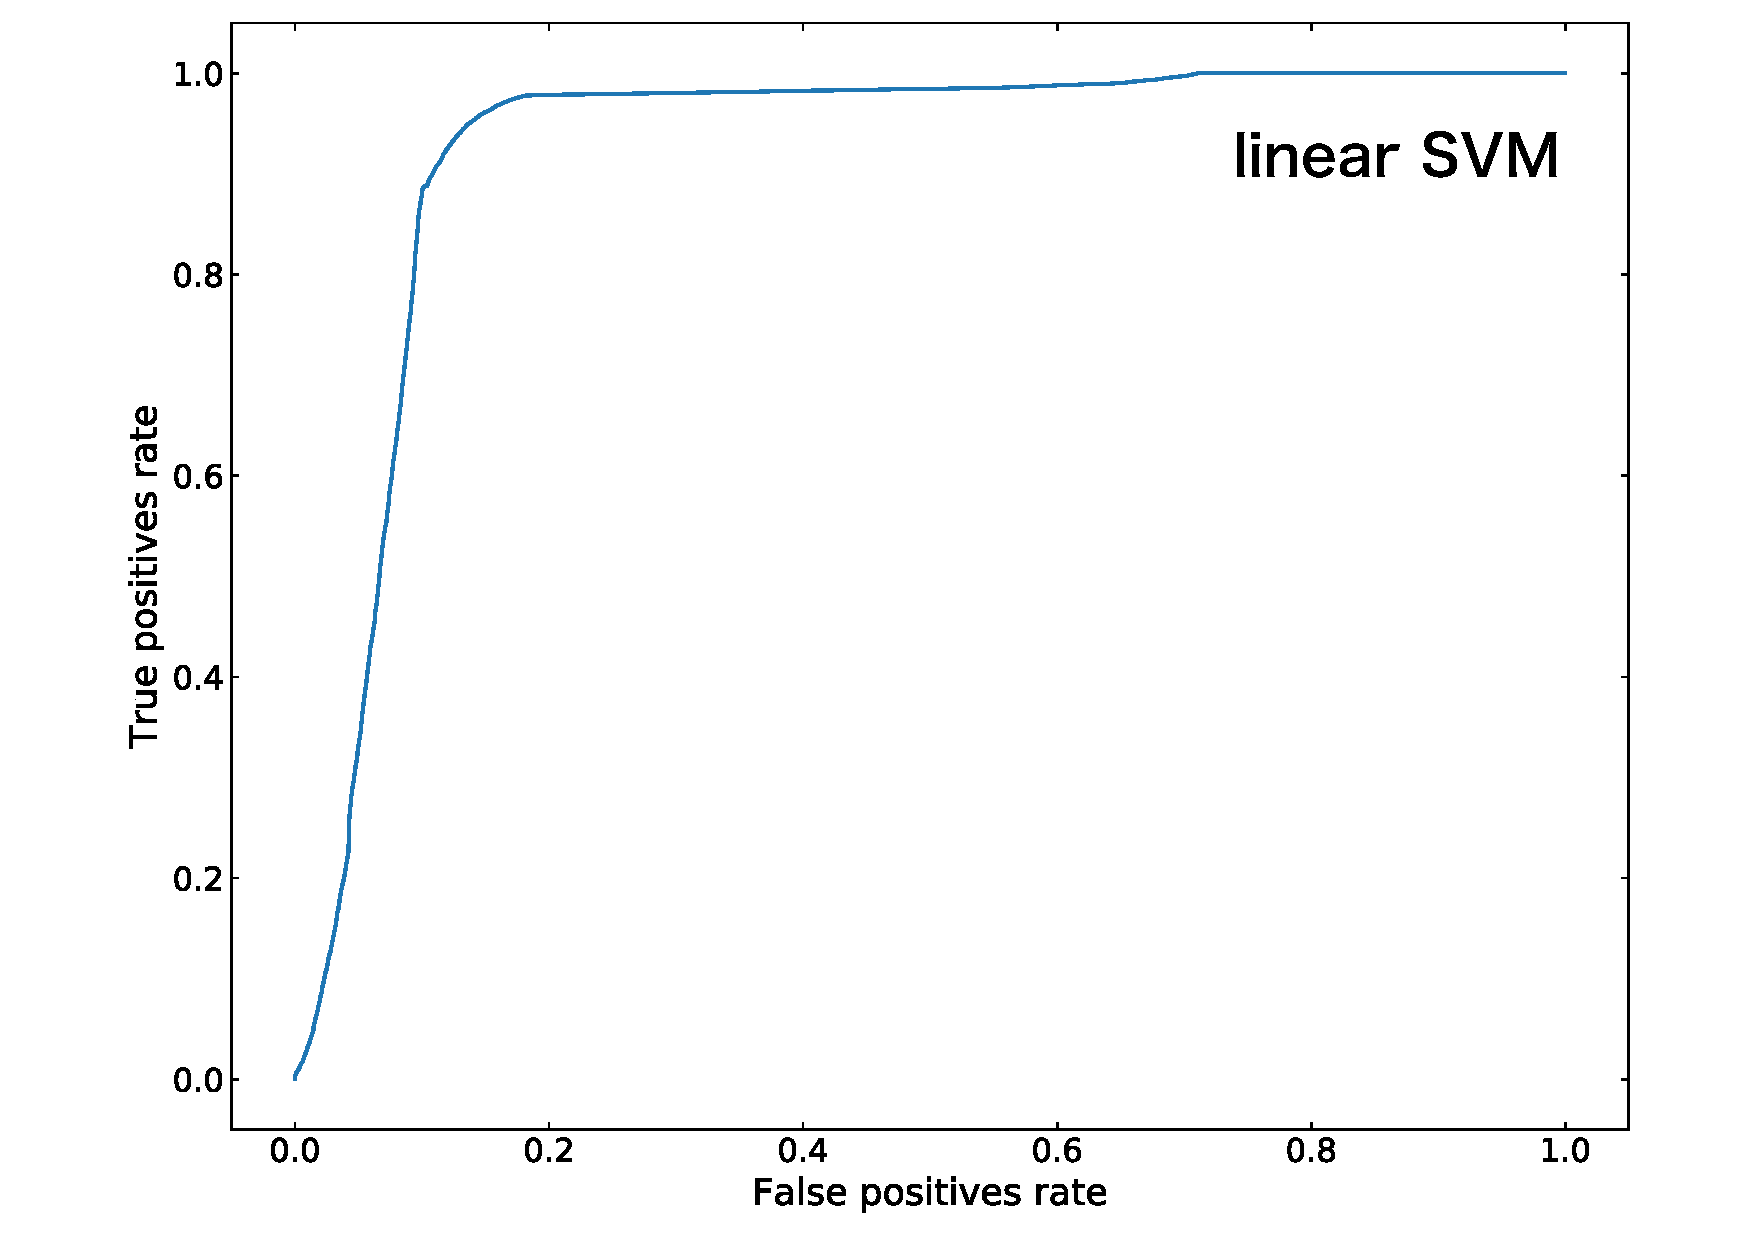
\includegraphics[width=0.5\textwidth]{Fig/fig_HGCAL/ROC-2vars-SVM}~
    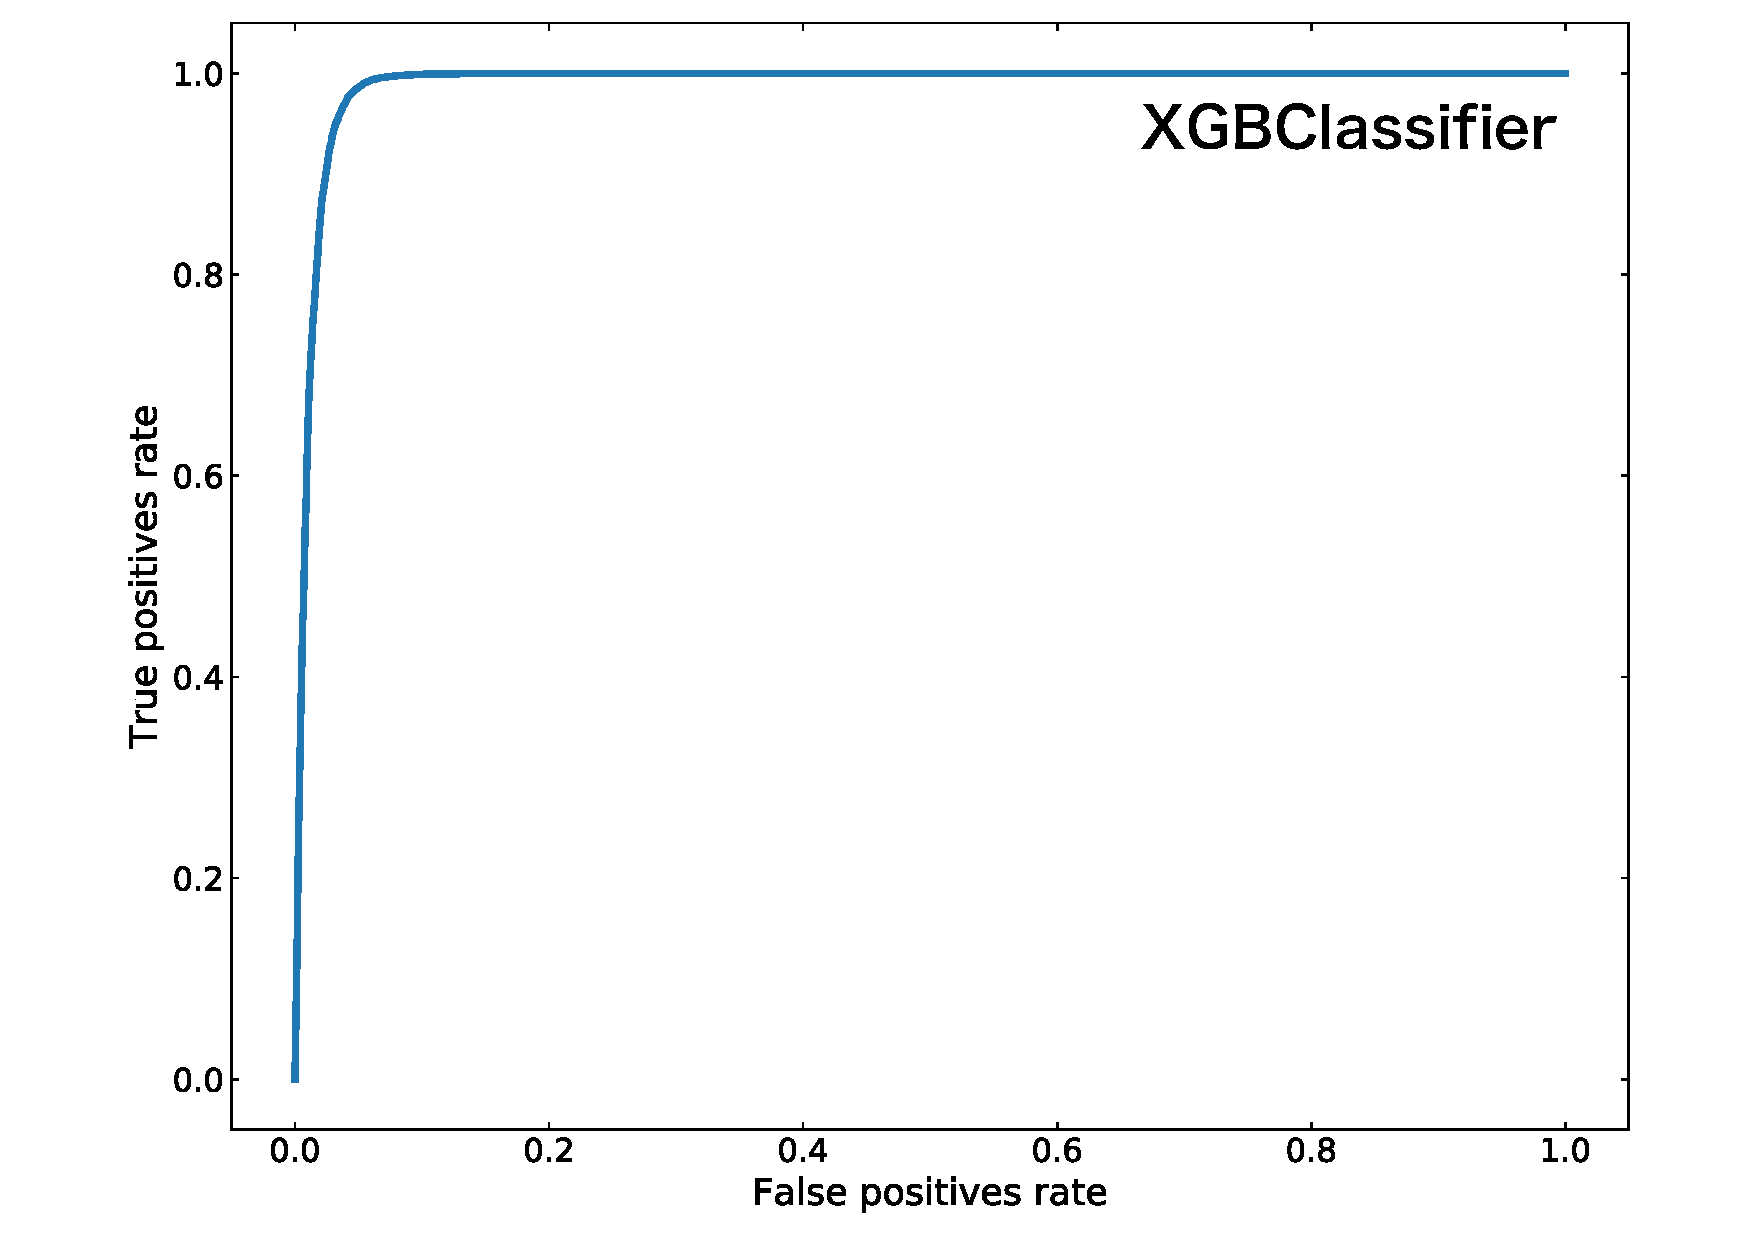
\includegraphics[width=0.5\textwidth]{Fig/fig_HGCAL/ROC-2vars-XGBClassifier}\\
    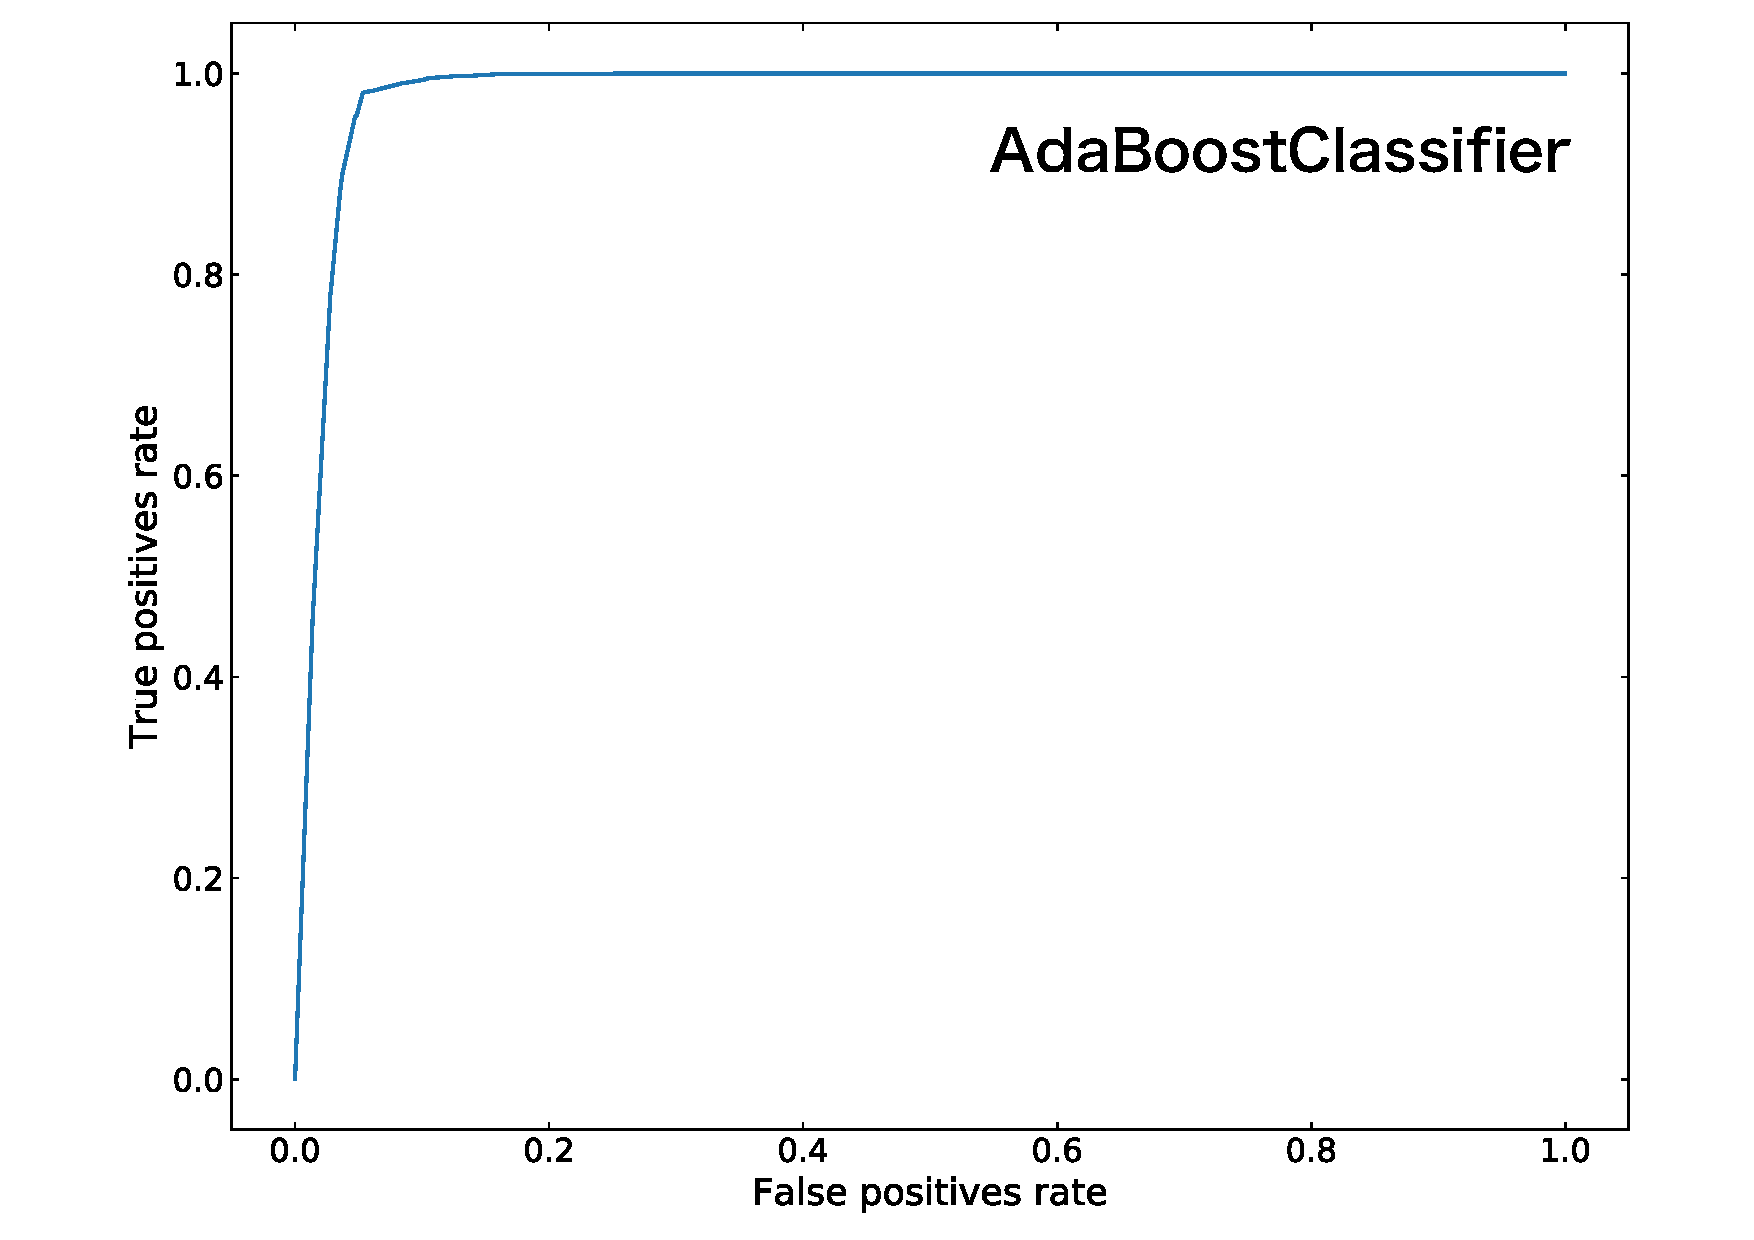
\includegraphics[width=0.5\textwidth]{Fig/fig_HGCAL/ROC-2vars-AdaBoost}~
    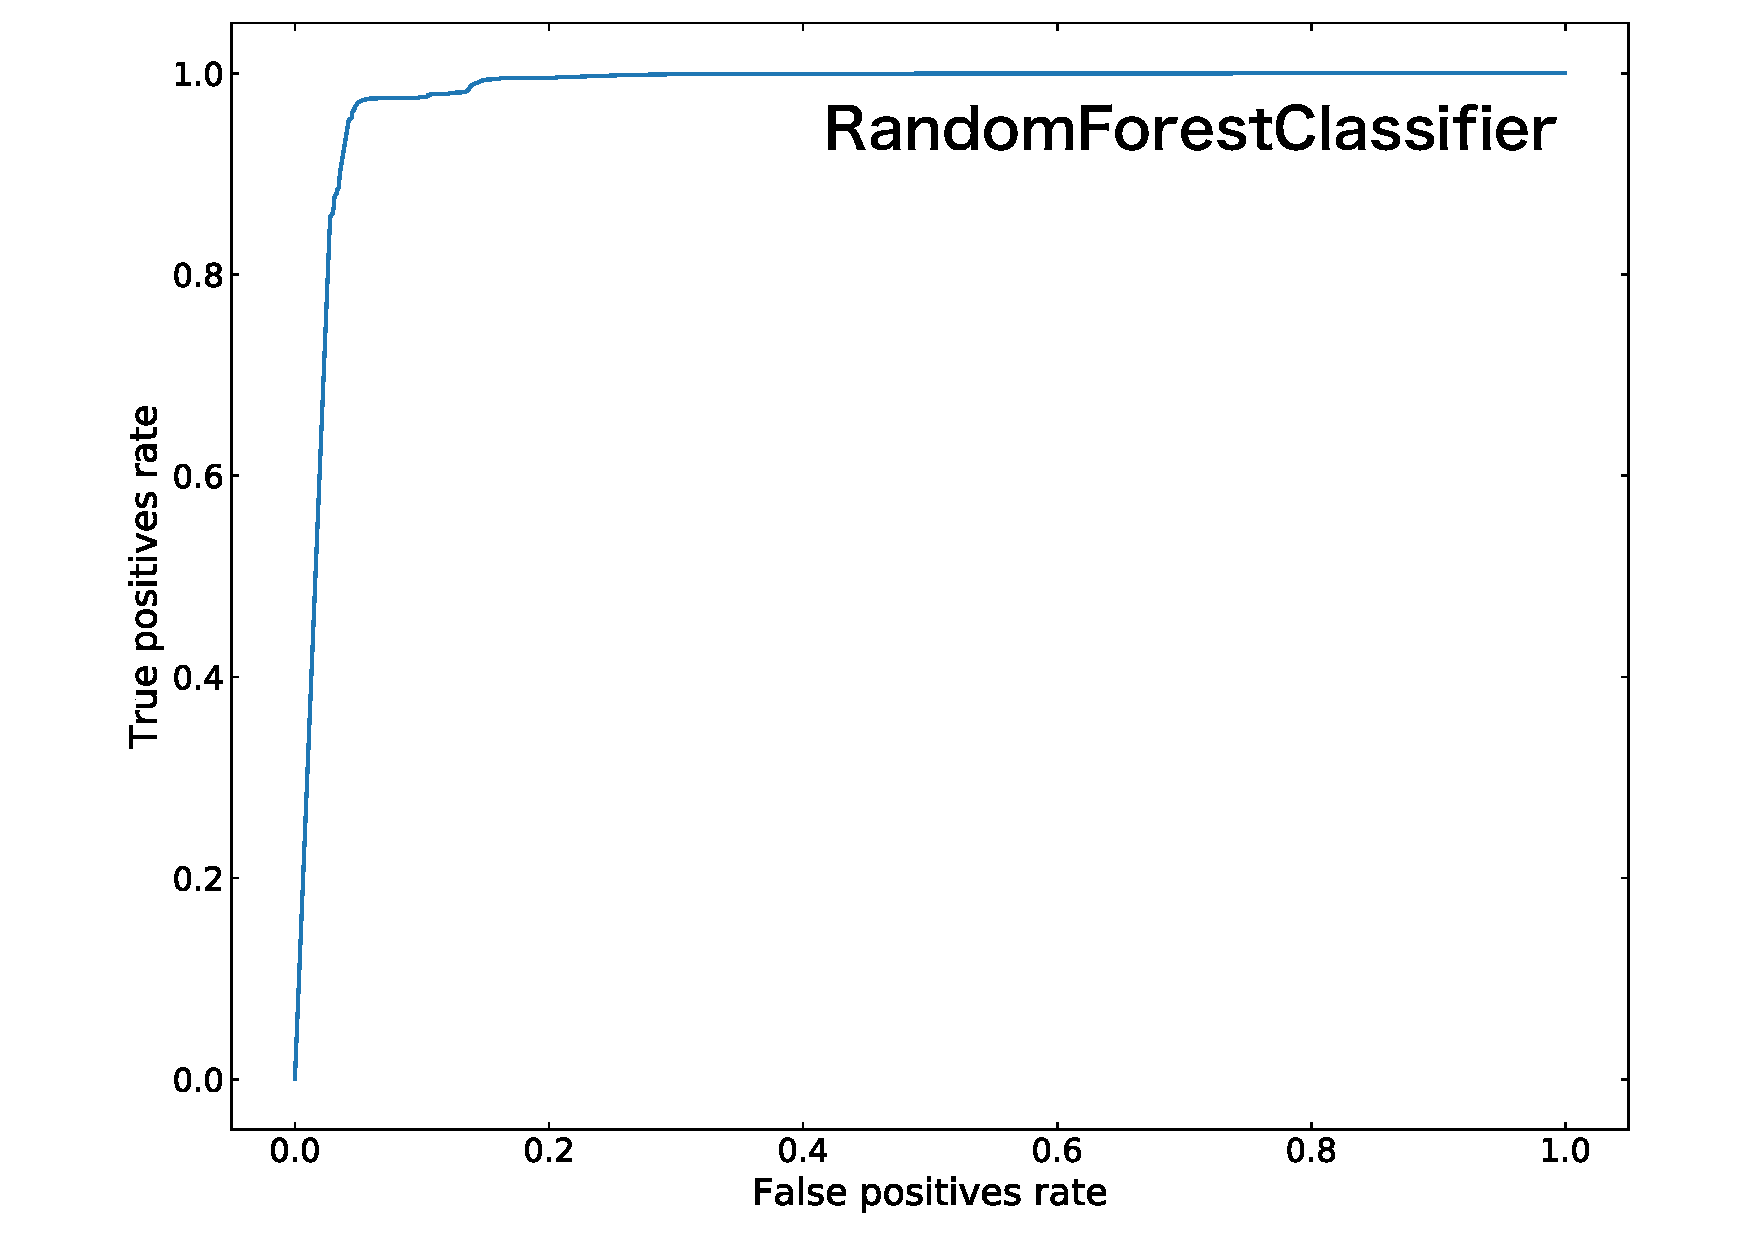
\includegraphics[width=0.5\textwidth]{Fig/fig_HGCAL/ROC-2vars-RandomForest}\\1
    \caption{ROC curves from linear SVM (top left), XGBClassifier (top right), AdaBoostClassifier (bottom left), RandomForestClassifier (bottom right).}
    \label{fig:ROCcurves}
    \end{center}
\end{figure}

\begin{table}[!ht]
  \begin{center}
    {
    \begin{tabular}{cc}
    	Classifier &  Background efficiency (with 99.0\% of signal efficiency) \\
    	\hline
    	XGBClassifier & 5.43 \\
    	AdaBoostClassifier  & 8.40 \\
    	RandomForestClassifier & 14.2 \\
    	linear SVM & 64.9 \\
    \end{tabular}
    }
  \end{center}
  \caption{The background (pion) efficiencies from tested classifiers with 99.0\% of signal (electron) efficiency.  \label{tab:ROC-summary}}
\end{table}


The next study is to add in more variables as training features. Different sets of training features are used, which are summarized as below.
\begin{enumerate}
\item Baseline (mdn of RecHit and depthX0) + Number of hits in all layers, referred to as nhits, or sum over all energy deposits in all layers
\item 4 variables - Baseline + nhits + Etot
\item 7 variables - Baseline + nhits + Etot + 3 variables, where the 3 variables are 
	\begin{itemize}
	\item The ratio of the energy sum in first two layers over Etot, referred to as \\ L1\_L2\_EAll\_over\_ETotal in the following figures.
	\item The ratio of the energy sum in first three layers over Etot, referred to as \\ L1\_L3\_EAll\_over\_ETotal in the following figures.
	\item The ratio of the energy sum in first ten layers over Etot, referred to as \\ L1\_L4\_EAll\_over\_ETotal in the following figures.
	\end{itemize}
\item 28 variables listed in Table.~\ref{tab:regression_feature}
\item 35 variables - Baseline + nhits + Etot + 3 variables + 28 variables listed in Table.~\ref{tab:regression_feature}
\end{enumerate}  

Fig.~\ref{fig:featimp-vars} shows the respect feature importances from different trainings listed above. For the trainings with 7, 28, and 35 variables, only the results from the combination of variables that give the best performance are shown. Interestingly, Etot is always the most important variable in the trainings where it is used. The correlation matrices of 35 variables from electron and pion events are shown in Fig.~\ref{fig:corr-matrix-35vars}.

\begin{figure}[p]
    \begin{center}  
    \includegraphics[width=0.5\textwidth]{Fig/fig_HGCAL/featimp-2vars-XGBClassifier}~
    \includegraphics[width=0.5\textwidth]{Fig/fig_HGCAL/featimp-3vars-v2-XGBClassifier}\\
    \includegraphics[width=0.5\textwidth]{Fig/fig_HGCAL/featimp-3vars-XGBClassifier}~
    \includegraphics[width=0.5\textwidth]{Fig/fig_HGCAL/featimp-4vars-XGBClassifier}\\
    \includegraphics[width=0.5\textwidth]{Fig/fig_HGCAL/featimp-7vars-v6-XGBClassifier}~
    \includegraphics[width=0.5\textwidth]{Fig/fig_HGCAL/featimp-28vars-v7-XGBClassifier}\\
    \includegraphics[width=0.5\textwidth]{Fig/fig_HGCAL/featimp-35vars-v6-XGBClassifier}~
    \caption{The respect feature importances from different trainings, as listed previously in the text.}
    \label{fig:featimp-vars}
    \end{center}
\end{figure}

\begin{figure}[p]
    \begin{center}  
    \includegraphics[width=0.67\textwidth]{Fig/fig_HGCAL/corr_matrix_35vars_v14-electron}\\
    \includegraphics[width=0.67\textwidth]{Fig/fig_HGCAL/corr_matrix_35vars_v14-pion}\\
    \caption{The correlation matrix of the training features for 35 variables.}
    \label{fig:corr-matrix-35vars}
    \end{center}
\end{figure}

Fig.~\ref{fig:FPrate-Nvar} shows the background efficiencies with different sets of 28 variables listed in Table.~\ref{tab:regression_feature}. From the left plot, the combination [Baseline + nhits + Etot + 3 variables + 28 E1 variables] so far gives the best performance among all tested combinations. From both plots, one can see that including lateral shower shape variables does not seem helpful on discriminating the electron and pion events.

\begin{figure}[!ht]
    \begin{center}  
    \includegraphics[width=0.5\textwidth]{Fig/fig_HGCAL/Nvar28-FPrate-XGBClassifier}~
    \includegraphics[width=0.5\textwidth]{Fig/fig_HGCAL/Nvar35-FPrate-XGBClassifier}\\
    \caption{The background efficiencies with different sets of 28 variables listed in Table.~\ref{tab:regression_feature}.}
    \label{fig:FPrate-Nvar}
    \end{center}
\end{figure}

Table.~\ref{tab:performance-summary} summarizes the performances from different sets of training features listed previously in the text. With the machine learning technique, the baseline identification gives 28.6\% improvement with respect to the window cut. From the fact that adding only the Etot brings approximately 90\% of improvement and the feature importances, one can conclude that Etot is a critical variables in the electron and pion discrimination. However, when adding 28 variables, the improvement seems marginal. The next step is to perform hyper-parameter optimization and see if the improvement is actually limited by the default setting of the hyper-parameter. Another issue is that there are huge number of variables that can be used in the training, and dumping all the variables into the training seems redundant. How to choose training features to give optimal performance should be dedicated.   

\begin{table}[!ht]
  \begin{center}
    {\scriptsize
    \begin{tabular}{ccccc}
    	Features &  Number of training features & Background efficiency (\%) & Improvement (\%) & Improvement (\%) \\
    		& 	& (at 99\% of signal efficiency) & w.r.t window cut & w.r.t baseline \\
    	\hline
    	Window cut & 2 & 7.60 & --- & --- \\
    	Baseline & 2 & 5.43 & 28.6 & --- \\
    	Baseline + nhits & 3 & 2.81 & 63.0 & 48.3 \\
    	Baseline + Etot & 3 & 0.613 & 91.9 & 88.7 \\
    	4 variables & 4 & 0.562 & 92.6 & 89.7 \\
    	7 variables &  7 & 0.427 & 94.4 & 92.1 \\
    	28 variables &  28 & 0.464 & 93.9 & 91.5 \\
    	35 variables & 35 & 0.359 & 95.3 & 93.4\\
    \end{tabular}
    }
  \end{center}
  \caption{Summary of the performances from different sets of training features. \label{tab:performance-summary}}
\end{table}